%
% -------- COMPILAR CON XELATEX -----------
%

\documentclass[a4paper,fleqn]{book}
%===============================================================================
% Configuracion de pagina
\usepackage[a4paper,
twoside,
hmargin={2cm,2cm},
vmargin={2cm,2cm},
bindingoffset=1cm]{geometry}
\setcounter{secnumdepth}{3}
%===============================================================================
% Idioma
%\usepackage[spanish]{babel}
%\decimalpoint
%===============================================================================
% Paquetes para fuentes
\usepackage{amsfonts}
\usepackage{amsmath}
\usepackage{amssymb}
\usepackage{mathtools}
\usepackage{amsthm}
\usepackage{bm}
\usepackage{wasysym}
\usepackage{eurosym}
\usepackage{textcomp}
\usepackage{url}      % Poner URL con enlace en el pdf y formatear
\usepackage{etex}     % Para memoria dinamica - listings
\reserveinserts{28}   % Para memoria dinamica - listings
\usepackage{listings} % Codigo fuente y algoritmos
% Tipo de letra sans serif
% Ver web: http://dtrx.de/od/tex/sfmath.html
% Descomentar esta linea
%\usepackage{cmbright}
% O bien descomentar estas dos lineas
%\renewcommand{\familydefault}{\sfdefault} % letra sans serif
%\usepackage{sfmath} % math en sans serif
% Tipo de letra parecida a Elsevier
%\usepackage{fourier}
% Letra times
%\usepackage{mathptmx}
% %===============================================================================
% % Imagenes, figuras y tablas
\usepackage[table,x11names]{xcolor}
\usepackage{booktabs}        % Reglas para tablas
\usepackage{longtable}       % Tablas en varias paginas
\setcounter{LTchunksize}{30} % Ajustar chunks para el paquete longtable
\usepackage{ltabptch}        % Bug longtable
\usepackage{rotating}        % Girar figuras y tablas sideways
\usepackage{lscape}          % Paquete para girar tablas y ocupar varias paginas
\usepackage{colortbl}        % Coloreado de tablas
\usepackage{multirow}        % Tratamiento celdas tablas
\usepackage{caption}
\usepackage{graphicx}
\graphicspath{{figures/}} %Setting the graphicspath
\usepackage{epsfig}
\usepackage{subcaption}
\usepackage{float}
\usepackage{subfloat}
\usepackage{multicol}
%\usepackage{subfig}          % Varias figuras en un flotante entre paginas
%\usepackage{pst-all}         % pstricks
%\usepackage{pstricks,framed} % pstricks dibujo frames
%\usepackage{tikz}            % Paquete grafico muy potente
% %===============================================================================
% % Decoracion del documento
\usepackage[explicit]{titlesec}              % Variables decorar cada chapter
\usepackage{fancyhdr}                        % Encabezados y pie de pagina.
\usepackage{fancybox}                        % Cajas alrededor de textos
\usepackage{fancyvrb}                        % Verbatim specials
\usepackage{enumerate}                       % Tipos de numeracion
\usepackage[footnote,printonlyused]{acronym} % Acronimos
%===============================================================================
% Indice de palabras
\usepackage{makeidx}
\makeindex
%===============================================================================
\usepackage{hyperref} % si se utiliza, comentar subfig
\usepackage{cleveref}

\renewcommand{\arraystretch}{1.5}
\newcolumntype{L}[1]{>{\raggedright\let\newline\\\arraybackslash\hspace{0pt}}m{#1}}
\newcolumntype{C}[1]{>{\centering\let\newline\\\arraybackslash\hspace{0pt}}m{#1}}
\newcolumntype{R}[1]{>{\raggedleft\let\newline\\\arraybackslash\hspace{0pt}}m{#1}}


\title{

\includegraphics[width=4cm]{../../docs/img/logo.pdf}
\\
MultiFEBE (version 2.0.0)
\\
Reference Manual}
\author{

}
\date{July 2022}

\begin{document}

\maketitle

\cleardoublepage

\chapter*{Copyright Notice and Disclaimers}

\begin{large}
Copyright {\copyright} 2014-2022 Universidad de Las Palmas de Gran Canaria
\\\\
Jacob D.R. Bordón \\ 
Guillermo M. \'Alamo \\
Juan J. Azn\'arez \\
Orlando Maeso
\\\\
This program is free software: you can redistribute it and/or modify it under the terms of the GNU General Public License as published by the Free Software Foundation, either version 2 of the License, or (at your option) any later version.
\\\\
This program is distributed in the hope that it will be useful, but WITHOUT ANY WARRANTY; without even the implied warranty of MERCHANTABILITY or FITNESS FOR A PARTICULAR PURPOSE. See the GNU General Public License for more details.
\\\\
Proper acknowledgment should be given in publications resulting from the use of these software.
\end{large}

\cleardoublepage

\chapter*{Acknowledgments}

We would like to thank all the code users through the years, in particular to María Castro, María José Orjuela, Francisco González, Carlos Romero, and especially to Ángel Gabriel Vega, who is giving momentum to the project and it is the author of the tutorials. Their experience have been very valuable for debugging and developing the software. We would like to make a special mention to Luis Alberto Padrón for pushing and supporting this open source enterprise from many angles.

\begin{figure*}[bh]
This software has been developed with the support of research projects: 
\begin{itemize}
    \item PID2020-120102RB-I00, funded by the Agencial Estatal de Investigaci\'on of Spain, \\ MCIN/AEI/10.13039/501100011033.
    \begin{center}
    \includegraphics[scale=0.9]{figures/miciinn-aei.png}
    \end{center}
    \item ProID2020010025, funded by Consejer\'ia de Econom\'ia, Conocimiento y Empleo (Agencia Canaria de la Investigaci\'on, Innovaci\'on y Sociedad de la Informaci\'on) of the Gobierno de Canarias and FEDER.
    \begin{center}
    \includegraphics[scale=0.9]{figures/miciinn-feder-aei.png}
    \end{center}
    \item BIA2017-88770-R, funded by Subdirecci\'on General de Proyectos de Investigaci\'on of the Ministerio de Econom\'ia y Competitividad (MINECO) of Spain and FEDER.
    \begin{center}
    \includegraphics[scale=0.9]{figures/gobcan-fse.png}
    \end{center}
\end{itemize}
\end{figure*}

\tableofcontents

\chapter{Overview}

In this chapter, a brief overview of MultiFEBE download, install and usage is given. Since MultiFEBE is open source (GPLv2 license), it can also be compiled by you, see Appendix \ref{ap:compilation}.

\section{Introduction}

MultiFEBE is a solver for performing linear elastic static and time harmonic analyses of continuum and structural mechanics problems comprising multiple interacting regions. It is based on the Finite Element Method (FEM) and the Boundary Element Method (BEM), which are combined in order to offer many advanced features not found elsewhere. These distinctive features have been published in many scientific papers, from which \cite{maeso2004,aznarez2006,padron2007,alamo2016,bordon2017} can be highlighted. No doubt, this program is heir to boundary element codes published by Professor Jose Dom\'inguez \cite{dominguez1993}.

Linear elastic solid materials are available for regions modeled by finite elements or boundary elements in static and time harmonic analysis, whereas linear poroelastic (Biot's theory) and inviscid fluid materials are available only for regions modeled by boundary elements in time harmonic analysis (wave propagation problems).

It has a full set of linear elastic finite elements: 
\begin{itemize}
    \item Solid (or continuum) finite elements:
    \begin{itemize}
        \item For two-dimensional plane strain / plane stress problems:
        \begin{itemize}
            \item 3 or 6 nodes triangular element.
            \item 4, 8 or 9 nodes quadrilateral element.
        \end{itemize}
        %
        % Under development
        %
        %\item For three-dimensional problems:
        %\begin{itemize}
        %    \item 4 or 10 nodes tetrahedral element.
        %    \item 8, 20 or 27 nodes hexaedral element.
        %\end{itemize}
    \end{itemize}
    \item Structural finite elements:
    \begin{itemize}
        \item 2D/3D bar element (2 nodes).
        \item 2D/3D beam elements (doubly symmetric cross-section):
        \begin{itemize}
            \item 2 or 3 nodes Euler-Bernoulli or Timoshenko straight element.
            \item 3 or 4 nodes curved element based on the degeneration from solid (Timoshenko theory).
        \end{itemize}
        \item 3D shell elements (Reissner-Mindlin theory):
        \begin{itemize}
            \item 3 or 6 nodes triangular shell element based on the degeneration from solid (full/selective/reduced integration).
            \item 4, 8 or 6 nodes quadrilateral shell element based on the degeneration from solid (full/selective/reduced integration).
            \item 9 nodes quadrilateral MITC element (locking-free).
        \end{itemize}
    \end{itemize}
    \item Discrete finite elements:
    \begin{itemize}
        \item 2D/3D discrete translational and translational-rotational spring/dashpot 2 node elements.
        \item 2D/3D mass elements.
    \end{itemize}
\end{itemize}

It also has a full set of boundary elements for linear elastic solids, poroelastic media and inviscid fluids:
\begin{itemize}
    \item For two-dimensional plane strain / plane stress problems:
    \begin{itemize}
        \item 2, 3 or 4 line ordinary or crack boundary elements.
        \item 2, 3 or 4 line body load elements.
    \end{itemize}
    \item For three-dimensional problems:
    \begin{itemize}
        \item 3 or 6 triangular ordinary or crack boundary elements.
        \item 4, 8 or 9 quadrilateral ordinary or crack boundary elements.
        \item 2, 3 or 4 line body load elements (only in elastic regions).
        \item 3 or 6 triangular body load elements.
        \item 4, 8 or 9 quadrilateral body load elements.        
    \end{itemize}
\end{itemize}

Finite elements can be coupled to ordinary boundary, crack boundary and body load elements in order to study Soil-Structure, Fluid-Structure and Soil-Fluid-Structure Interaction in wave propagation problems. This type of mcoupling

Figure \ref{fig:owt} shows an example of the modeling capabilities, where an Offshore Wind Turbine installed on a jacket structure founded on suction caissons. Finite elements model the whole foundation and structure, which includes additional masses in order to incorporate Water-Structure Interaction, and boundary and body load elements (geometrically coincident with suction caissons skirts and lids) for modeling Soil-Structure Interaction. Soil free-surface discretization is not shown for the sake of clarity.

\begin{figure}[h]
\centering
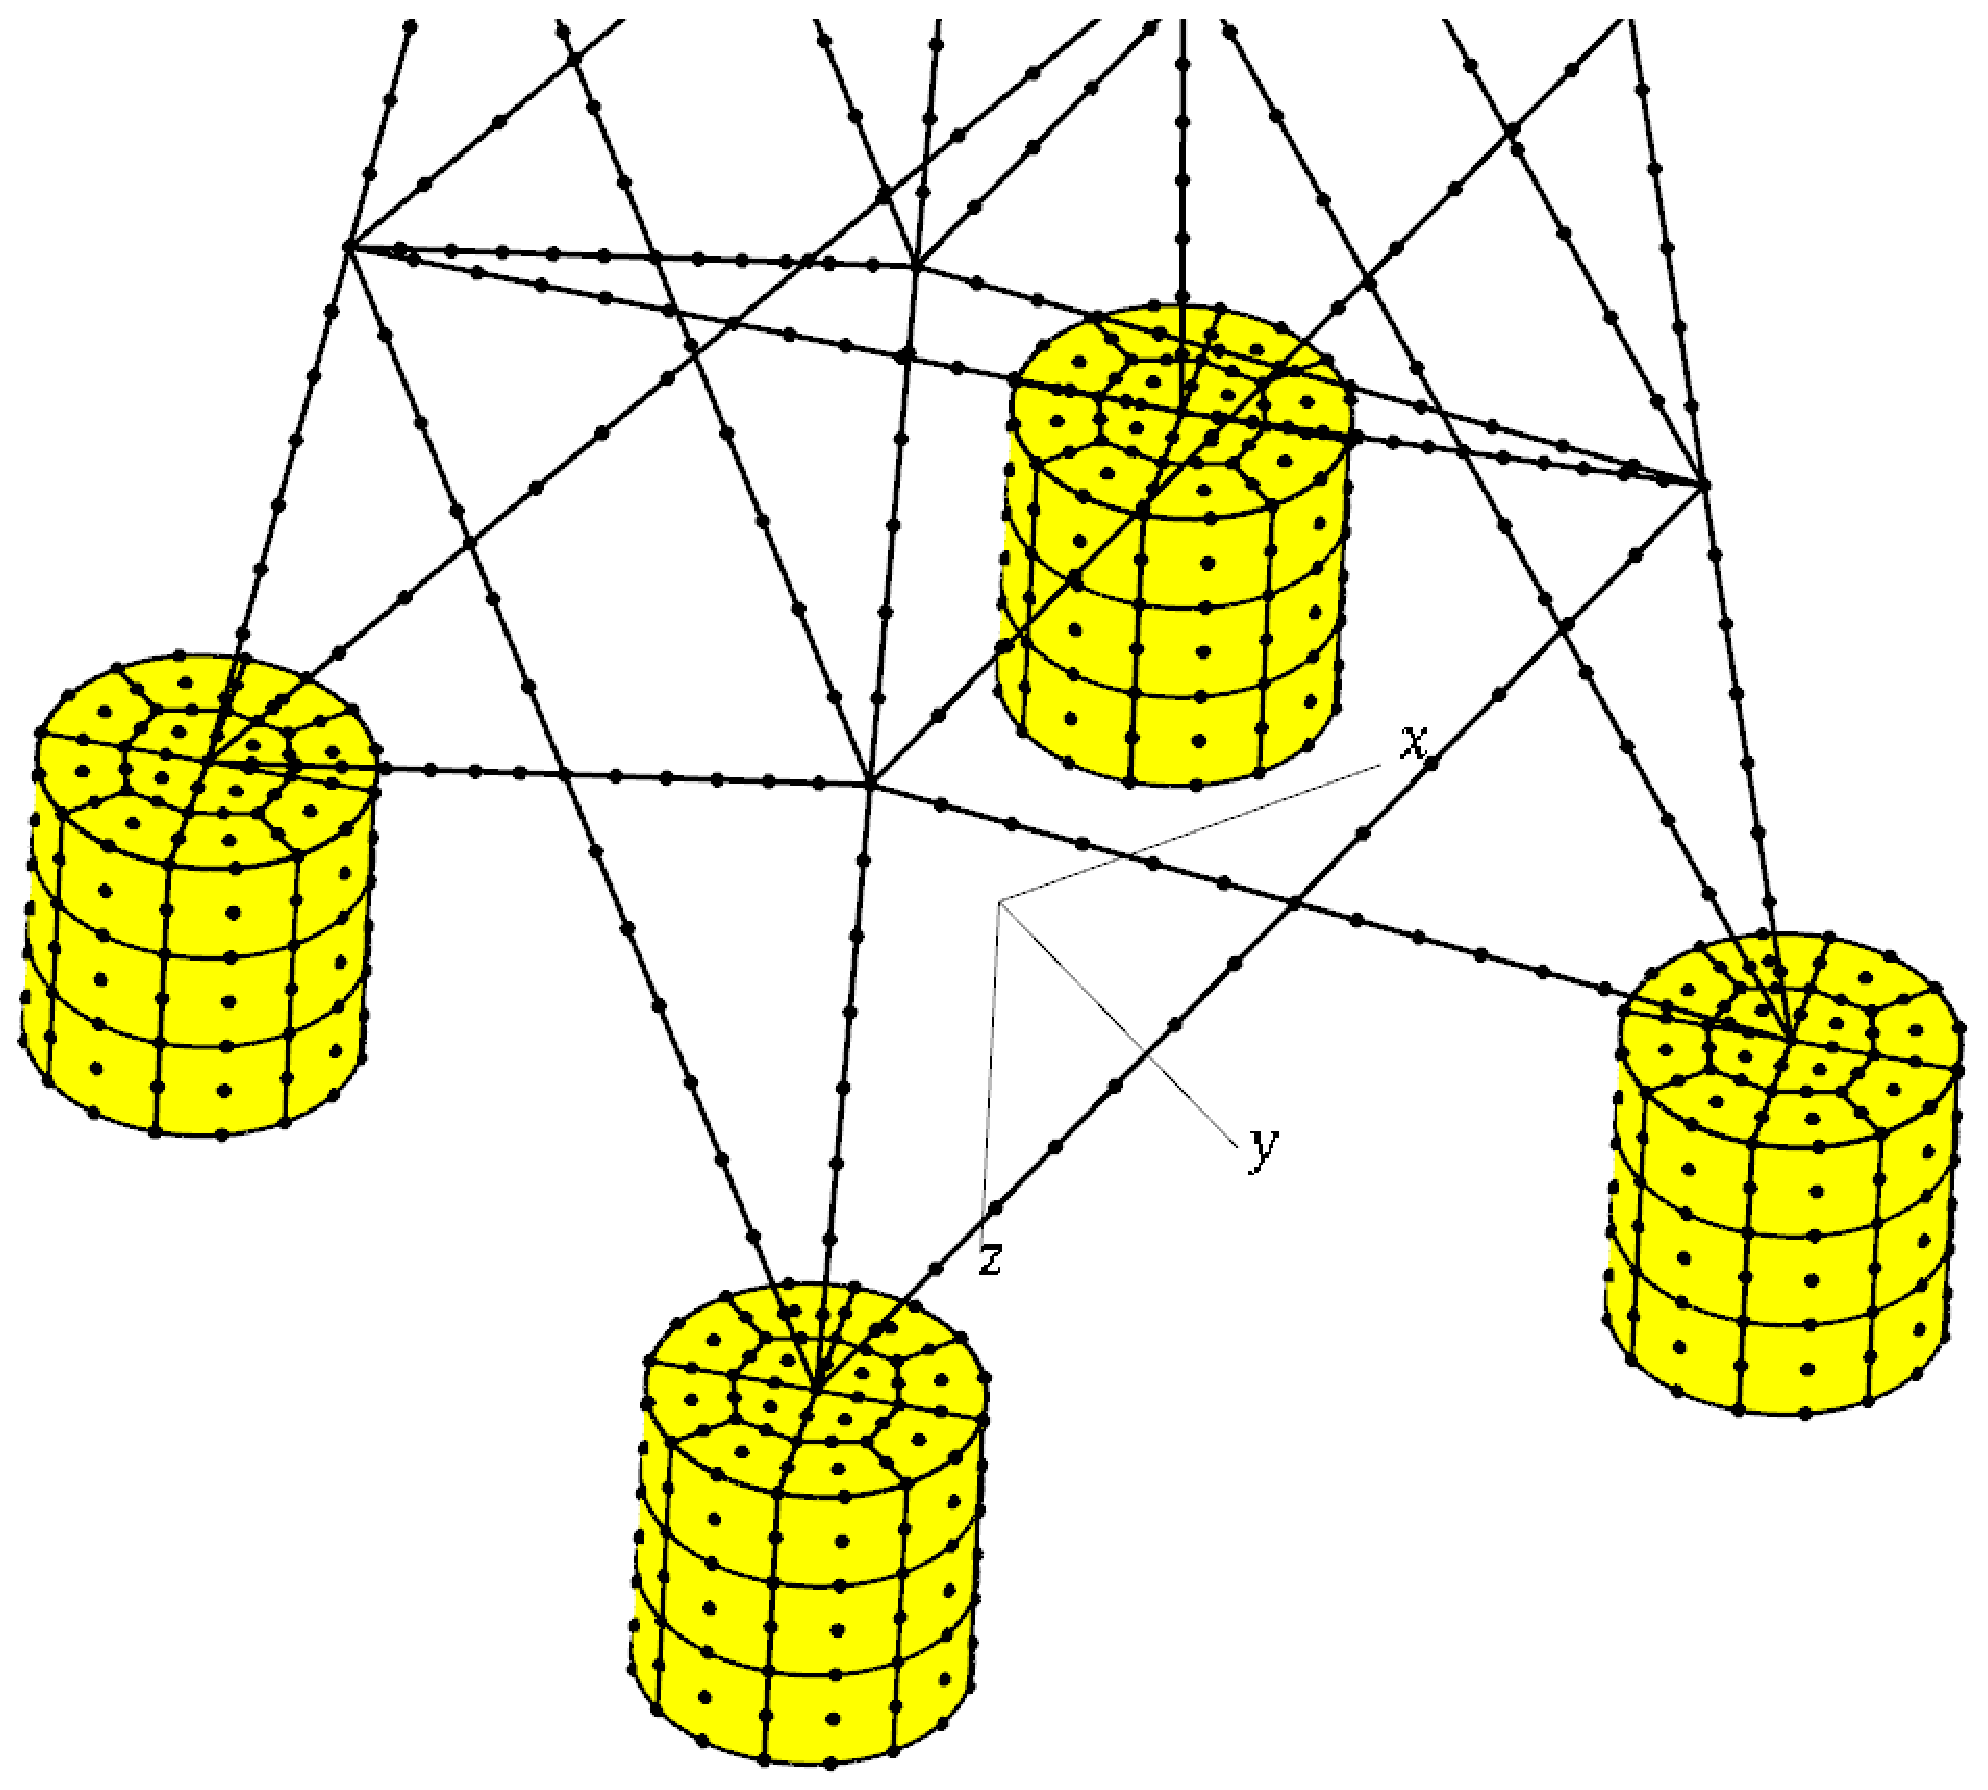
\includegraphics[width=0.6\textwidth]{figures/shell_fe.eps}
\caption{Jacket-based Offshore Wind Turbine founded on suction caissons}
\label{fig:owt}
\end{figure}


%
% To be written
%
%The solver is also able to perform geometric sensitivity analyses (currently only 2D).

%
% To be written
%
%\section{A little bit of history}

\section{How to download}

The \textbf{binaries} and the \textbf{source code} of MultiFEBE are available at the \href{http://www.mmc.siani.es/}{research group webpage} and at \href{https://github.com/mmc-siani-es/MultiFEBE}{GitHub}. MultiFEBE is released under \href{https://github.com/mmc-siani-es/MultiFEBE/blob/main/LICENSE}{GPLv2} license. That means that you may copy, distribute and modify the software as long as you track changes/dates in source files. Also, any modifications to or software including (via compiler) GPL-licensed code must also be made available under the GPL along with build \& install instructions.

MultiFEBE is available for GNU/Linux and Windows 64-bit operating systems. Binaries are released in \texttt{*.deb} and \texttt{*.sh} installer packages for GNU/Linux, and in an \text{*.exe} installer for Windows. Source code can be compiled using \texttt{cmake} + \texttt{make} + \texttt{gfortran} in GNU/Linux, and through \texttt{MSYS2}/\texttt{mingw-w64} + \texttt{cmake} + \texttt{make} + \texttt{gcc-fortran}. The program requires multi-core linear algebra libraries: ATLAS or OpenBLAS; which are successors of single-core LAPACK and BLAS. OpenBLAS is the default choice as it can easily be used in both GNU/Linux and Windows. The whole package is configured as a static build, i.e. the program is statically linked against libraries. Details about installing are given below. 


\section{How to install the binaries}

\subsection{GNU/Linux \texttt{*.deb} installer}

\label{subsec:deb}

The installation steps are:
\begin{enumerate}
    \item Go to \href{https://github.com/mmc-siani-es/MultiFEBE/releases}{GitHub}, and download the most recent \texttt{*.deb} release.
    \item Make double-click on the installer.
    \item Press the install button, and then type your password in the authentication window.   
\end{enumerate}

\subsection{GNU/Linux \texttt{*.sh} installer}

The installation steps are:
\begin{enumerate}
    \item Go to \href{https://github.com/mmc-siani-es/MultiFEBE/releases}{GitHub}, and download the most recent \texttt{*.sh} release (e.g. \texttt{multifebe-x.x.x-Linux.sh}).
    \item Press Ctrl+Alt+T to open a terminal, and navigate to the folder where it has been downloaded.
    \item Change the permissions of the file to allow its execution:
\begin{Verbatim}[frame=single, fontsize=\small]
$ chmod +x multifebe-x.x.x-Linux.sh
\end{Verbatim}
    \item Now, you can execute the installer:
\begin{Verbatim}[frame=single, fontsize=\small]
$ ./multifebe-x.x.x-Linux.sh
\end{Verbatim}
    \item The program files are decompressed by default in the same directory as the installer. The executable file is placed inside the subfolder \texttt{bin}. You may copy or move the binary \texttt{multifebe} to any folder where you want to use it, and execute as \verb!./!\texttt{multifebe ...} or, if you have administrator privileges in your system, you might move the binary \texttt{multifebe} to \texttt{/usr/bin}, or create a simbolic link, so that it is available directly in the terminal as any other command. 
\end{enumerate}

For details about options and usage, see below section \textit{How to use}~\ref{sec:howto}.

%\subsection{Windows installer}
%
%\label{subsec:exe}
%
%The installation steps are:
%\begin{enumerate}
%    \item Go to \href{https://github.com/mmc-siani-es/MultiFEBE/releases}{GitHub}, and download the most recent Windows installer release \texttt{*.exe}.
%    \item Right-click on the installer, and \textbf{run the application as administrator}.
%    \item Follow the installer instructions, except in the step shown in Figure \ref{fig:install_exe_2}, where you have to add the directory to the system PATH in order to make the executable visible in the terminal.
%    \begin{figure}[h]
%    \centering
%    \includegraphics[width=0.6\textwidth]{figures/windows_exe_2.png}
%    \caption{Windows installer: Step 3}
%    \label{fig:install_exe_2}    
%    \end{figure}
%    \item Continue the installer steps up until the end.
%\end{enumerate}

\section{How to compile the source code}

The procedure to compile from the source code is explained in Appendix \ref{ap:compilation}.


\section{How to use}
\label{sec:howto}

MultiFEBE is a command-line program that you can run on a Windows terminal (cmd or PowerShell) or GNU/Linux terminal. Once installed, you can run it by executing \texttt{multifebe} from a terminal as we already mentioned at the end of the installation steps. The program execution command line is started by \texttt{multifebe} and followed by a set of arguments which tells the program on how to run (options). For instance, as we did before, if we execute:
\begin{Verbatim}[frame=single, fontsize=\small]
$ multifebe --help
\end{Verbatim}
it will then print a brief help about how to run it and the available options:
\begin{Verbatim}[frame=single, fontsize=\small]
$ multifebe --help
Usage:                                                                          
  multifebe [options]                                                         

Options:                                                                        
  -i, --input STRING        Input file name           [required]                
  -o, --output STRING       Output files basename     [default: input file name]
  -m, --memory INTEGER      Max. memory allowed (GB)  [default: 0 (unlimited)]  
  -b, --verbose INTEGER     Verbose level: 0-10       [default: 1]              
  -v, --version             Program version                                     
  -h, --help                This help                                           
\end{Verbatim}
Note that each option can start with one or two hyphens, followed by respectively the short or long name of the option. In the previous case, we could request help from the program by writing either \texttt{-h} or \texttt{--help}. Some options does not require a value like \texttt{-h} or \texttt{-v}, but other options require a string or a number, which are written after each of them. Options are self-descriptive from the program help, but more details are given in Table \ref{tab:options}.

\begin{table}[h]
\centering
\begin{tabular}{cccp{7cm}}
\multicolumn{2}{c}{\textbf{Option name}} &  &\\
\textbf{Short} & \textbf{Long} & \textbf{Argument} & \textbf{Description} \\
\midrule
\texttt{-i} & \texttt{--input} & \texttt{STRING} & \texttt{STRING} is a path to the plain text input file where the definition of the case is read. This option is thus mandatory.
\\
\texttt{-o} & \texttt{--output} & \texttt{STRING} & \texttt{STRING} is a path to the basename of the output files (plain text) where the results of the case are printed. This option is optional since the input file path is taken by default. The output files differ only in the extension of the file.
\\
\texttt{-m} & \texttt{--memory} & \texttt{INTEGER} & \texttt{INTEGER} is the maximum memory (in GB) allowed to be used by the program when allocating the main matrices. If the program predicts that such memory (or more) is required, then it stops itself.  This option is important when dealing with large models in order to prevent the computer from memory swapping (transferring memory data to the hard-drive). Therefore, it is recommended to use this option with a setting of around 75\% of the available memory of the computer.
\\
\texttt{-b} & \texttt{--verbose} & \texttt{INTEGER} & \texttt{INTEGER} sets the level of details printed by the program when executing, being 0 the level where minimal information is printed and 10 the level where all the steps are printed.
\end{tabular}
\caption{MultiFEBE command-line arguments (options)}
\label{tab:options}
\end{table}

MultiFEBE uses \href{https://www.openmp.org/}{OpenMP} in order to take full advantage of multi-core shared-memory computers. By default, the program uses all the available cores, but it is possible to control the number of cores used by previously defining the environment variable \href{https://www.openmp.org/spec-html/5.0/openmpse50.html}{\texttt{OMP\_NUM\_THREADS}}. Imagine you would like to only use 4 cores, then in GNU/Linux you would have to execute:
\begin{Verbatim}[frame=single, fontsize=\small]
$ export OMP_NUM_THREADS=4
\end{Verbatim}
In Windows, it would have to execute:
\begin{Verbatim}[frame=single, fontsize=\small]
$ set OMP_NUM_THREADS=4
\end{Verbatim}

Figure \ref{fig:flowchart} shows a MultiFEBE usage flowchart. It operates mainly through plain text files. The program reads the input file in order to define the case (type of analysis, geometry topology, mesh, materials, boundary conditions, results to be calculated, etc). Results are written into a set of output files which depends on the type of results requested in the input file. 

%
% To be included
%
% For some problems, the user can establish the use of an auxiliary database file (in binary format) which allows reusing some computationally expensive calculations. 

\begin{figure}[h]
\centering
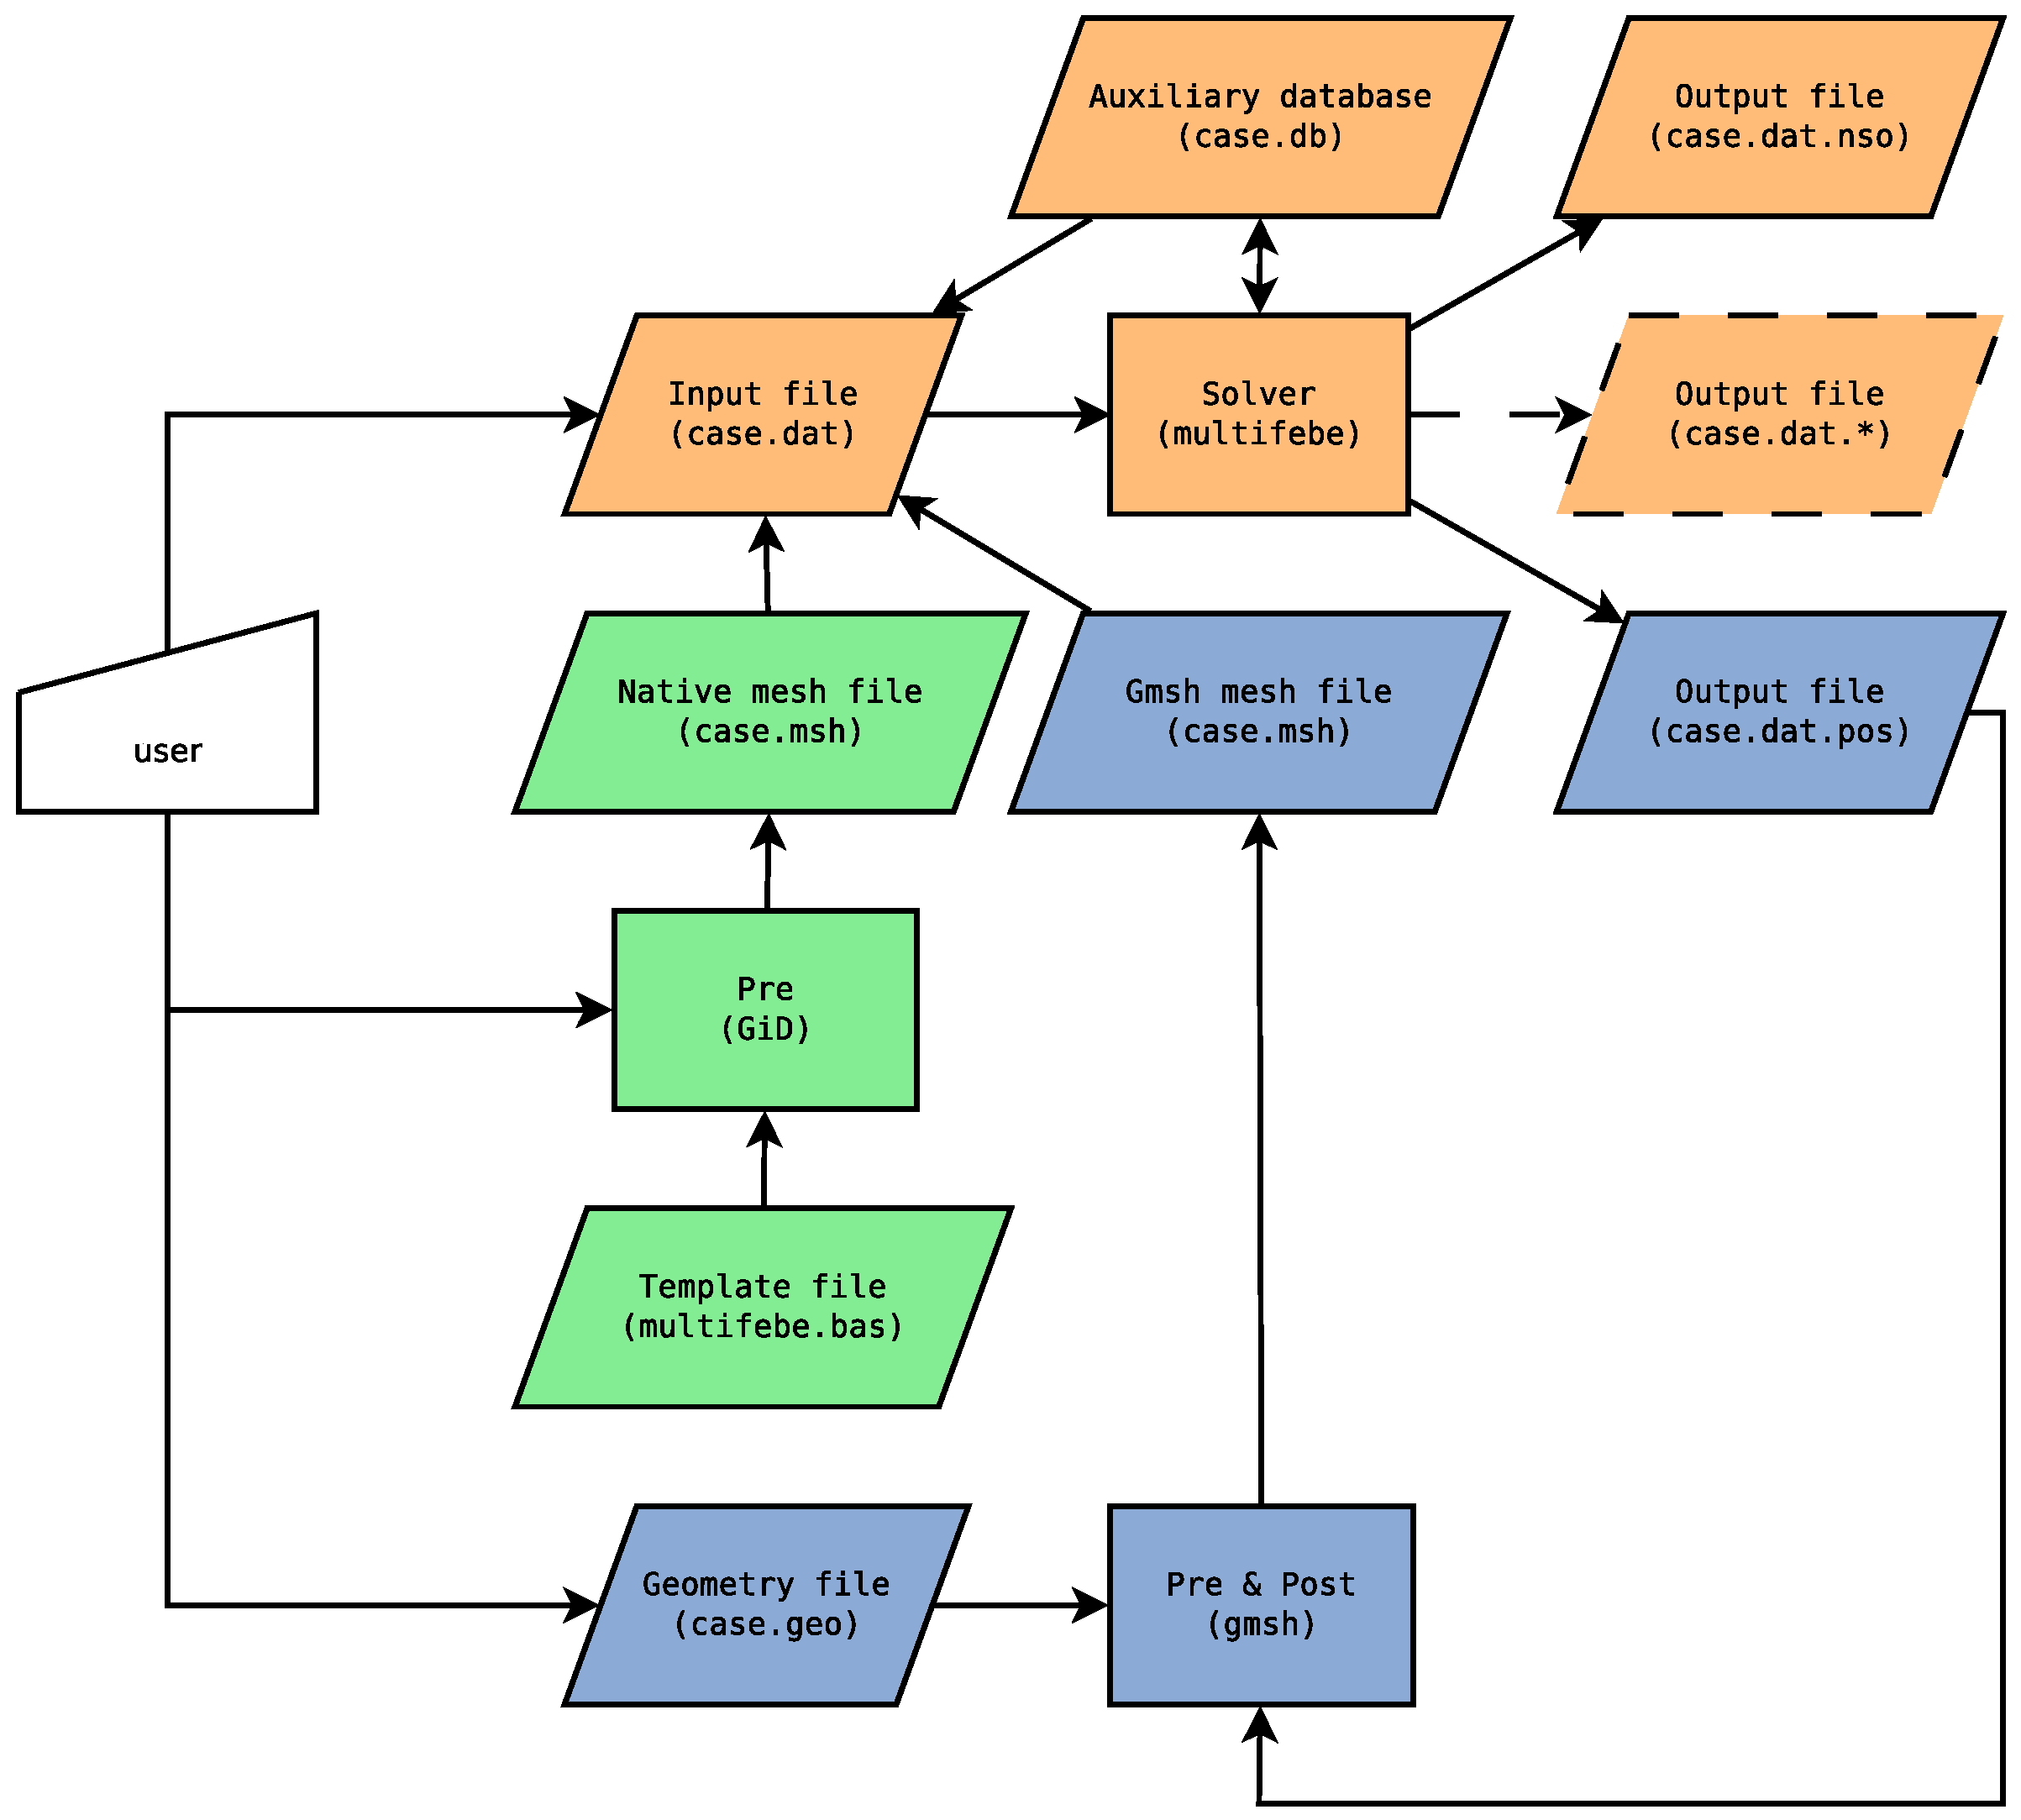
\includegraphics[width=\textwidth]{figures/Diagrama1.eps}
\caption{MultiFEBE usage flowchart. Orange blocks corresponds to MultiFEBE solver files and processes. Blue blocks corresponds to \href{https://gmsh.info}{Gmsh} pre- and post-processor files and processes. MultiFEBE is able to read Gmsh mesh files and write Gmsh postprocessing results files. Green blocks corresponds to the possibility of generating the mesh in MultiFEBE native format from \href{https://www.gidhome.com}{GiD} and a \texttt{*.bas} template file.}
\label{fig:flowchart}
\end{figure}

Most of the user effort is usually spent in preparing the geometry, mesh and then post-processing the results. In order to facilitate these tasks, we have included the possibility of reading and writing \href{https://gmsh.info}{Gmsh} files. \href{https://gmsh.info}{Gmsh} is a powerful free and open-source pre- and post-processor. The only Gmsh file format that MultiFEBE can read is MSH file format version 2.2, which is the default file format up to Gmsh 3.0.6. Newer Gmsh versions save mesh files in newer mesh file formats by default. However, you can also export meshes in older file format versions by doing \texttt{File>Export>Format: Mesh - Gmsh MSH (*.msh)>Format: Version 2 ASCII} when using the GUI, or including the option \texttt{-format msh2} when using the command-line. This integration enables the user to perform, for example, extensive parametric studies with relatively little extra effort, and effective visualization of results. We have also created a \href{https://www.gidhome.com}{GiD} \texttt{*.bas} template file which allows exporting the mesh file in the MultiFEBE native format (located in the \texttt{bin/} folder). We intend to improve the integration of MultiFEBE solver in GiD and others pre- and post-processors in the near future. In the same vein as \href{http://www.mmc.siani.es/software/piledyn}{PILEDYN}, we have also created some problem-specific \url{https://www.mathworks.com/}{MATLAB} pre- and post-processors that will be available in our \href{http://www.mmc.siani.es/software/}{research group webpage}.

The proposed workflow to perform an analysis is:
\begin{enumerate}
    \item Decide the modelling approach, which will lead to the required topology and geometry. We suggest using Gmsh for creating the geometry, which allows defining the geometry parametrically through simple \texttt{.geo} files.
    \item Generate the mesh with appropriate element sizes. In Gmsh, this can be easily done by defining element sizes all over the geometry using variables. Then you can set their value in order to generate a mesh. Once you have your solver results, you may have to return to this step to generate additional refined meshes in order to check results convergence.
    \item Open your favourite plain text text editor, and write the case input file according to the required data, as shown in Chapter \ref{ch:input_file}. If you use Gmsh for generating the mesh file, then you will have to define the path to it in section \texttt{[settings]}.
    \item Run the solver. Copy the solver executable to the folder where the case input file is located. Then, open a terminal in this folder and execute:
\begin{Verbatim}[frame=single, fontsize=\small]
$ multifebe -i case.dat
\end{Verbatim}
    where it has been assumed that the case input file is named \texttt{case.dat}. BEM models may require a huge amount of memory. We recommend that if the model is relatively big, or you are running the solver on a laptop, then you have to limit the available RAM for the program by including the following option:
\begin{Verbatim}[frame=single, fontsize=\small]
$ multifebe -i case.dat -m 4
\end{Verbatim}
    which will stop the solver if the predicted required memory is greater that 4 GB (or any other quantity smaller than the available memory in the computer). This will prevent the computer from swapping and halting if such amount of memory is required.
    \item Once the solver ends, the results are exported to one or more output files, see Chapter \ref{ch:output_files}. If you used a Gmsh mesh file (\texttt{*.msh}), Gmsh post-processing files \texttt{*.pos} will be generated. If that is the case, you can visualize the results in the Gmsh GUI. Other text files containing node-by-node, element-by-element, or other results can be generated (depending on how you set the case input file). This text files can be easily processed by spreadsheet programs, MATLAB/Octave, GNU utilities such as \text{awk}, etcetera. We recommend the latter, as it is particularly fast once you learn how to use it. They can also be plotted through GNU/Linux utilities such as GNUPlot.
\end{enumerate}

\chapter{Input file}

\label{ch:input_file}

\section{Introduction}

The input file is a \textbf{plain text} file which contains the \textbf{case data}. In the following, we will assume that the name of the input file name is \texttt{input.dat}, but any other name and extension will also be valid. The important fact is that the file \underline{must be a plain text file}, and thus it must be edited as such in plain text editors such as Notepad, \href{https://notepad-plus-plus.org/}{Notepad++} or others in Windows (but not Word or LibreOffice!), and emacs, gedit, vim or others in GNU/Linux environments.

The case data is divided into \textbf{sections}. Each section is a block of data related to an aspect of the case or the solver settings. Each section begins with a line exclusively containing a header with the section name between brackets, i.e. \texttt{[section name]}, and it ends when all the required data has been introduced or when another section header appears. It is important to note that its location within the file is not relevant. The data required for a section is defined by one or more lines after the header line. Each section has its own section format, which can be in the form of simple statements (\texttt{keyword = values}, \texttt{entity id: values}), or a sequence of numbers and strings. Only the recognized sections are read. Therefore, comments can be introduced outside the recognized ones (see example below). Recognized sections are shown in Table \ref{tab:section}. Some sections are required (mandatory), some sections are required depending on the data introduced in other sections (dependant), and others are completely optional.

\begin{Verbatim}[frame=single, fontsize=\small, label=input.dat]
[case description] <-- this is an unrecognized section used as a comment section
3x3 pile group analysis of stresses

[problem]
n = 3D
type = mechanics
analysis = harmonic

[frequencies]
Hz
lin
100
0.01
10.

[symmetry planes]
plane_zx: symmetry
plane_yz: antisymmetry

...
\end{Verbatim}

All the identifiers of model entities (regions, boundaries, elements, nodes, etc) must be integers greater than 0. Floating point numbers can be expressed as \texttt{125.} (simple precision), \texttt{1.25e2} (simple precision) or \texttt{1.25d2} (double precision). Complex numbers are expressed as \texttt{(2.d3,1.d1)}.

\begin{table}
{\footnotesize
\centering
\begin{tabular}{lL{7cm}L{2cm}}
\textbf{Section name} & 
\textbf{Brief description} & 
\textbf{Character} \\
\midrule
\multicolumn{3}{c}{\textit{General sections}} \\
\midrule
\texttt{problem}     & Type of problem, dimension $\mathbb{R}^n$ of the ambient space, and analysis to be performed & mandatory  \\
\texttt{frequencies} & Frequencies for a time harmonic analysis & dependent \\
\texttt{settings}    & Solver settings & optional  \\
\texttt{export}      & Export options and settings & optional  \\
\texttt{materials}   & Materials to be used in the model & optional \\
\midrule
\multicolumn{3}{c}{\textit{Low-level entities of the model (mesh) in native format}} \\
\midrule
\texttt{nodes}           & Nodes of the mesh                                            & dependant  \\
\texttt{elements}        & Elements of the mesh                                         & dependant  \\
\texttt{parts}           & Parts of the mesh (a connected set of elements of the same intrinsic dimension) & dependant  \\
\midrule
\multicolumn{3}{c}{\textit{High-level entities of the model (topology)}} \\
\midrule
\texttt{boundaries}    & Boundaries of BE regions (a part with elements of intrinsic dimension $\mathbb{R}^{n-1}$) & dependant  \\
\texttt{be body loads} & Body loads of BE regions (a part with elements of intrinsic dimension from 0D (point) to $\mathbb{R}^{n}$) & dependant  \\
\texttt{fe subregions} & Subregions of FE regions (a part with elements of intrinsic dimension $\mathbb{R}^n$ (solid) or lower (structure))     & dependant  \\
\texttt{cross sections} & Cross sections of the model. It contains data which complements the geometrical information contained in the mesh. It is required for structural elements. & dependant  \\
\texttt{regions}       & Regions (or subdomains) of the model & mandatory  \\
\midrule
\multicolumn{3}{c}{\textit{Auxiliary entities of the model}} \\
\midrule
\texttt{internal points} & Internal points of BE regions where the solution is calculated & optional  \\
\texttt{groups}          & Group of entities of the same class                            & optional  \\
\midrule
\multicolumn{3}{c}{\textit{Conditions throughout the model}} \\
\midrule
\texttt{symmetry planes}               & Symmetry planes of the model          & optional  \\
\texttt{conditions over be boundaries} & Boundary conditions of BE boundaries  & dependent \\
\texttt{conditions over fe elements}   & Boundary conditions of FE elements    & optional  \\
\texttt{conditions over nodes}         & Boundary conditions of BE or FE nodes & optional  \\
\texttt{incident waves}                & Input or incident wave fields         & dependant
\end{tabular}
\caption{Sections of the data file}
\label{tab:section}
}
\end{table}

\section{General sections}

\subsection{Section \texttt{problem}}

This section defines the main aspects of the case. It is composed of one or more unordered lines containing one assignment \texttt{keyword = values}. Table \ref{tab:problem} shows the recognized keywords, the values they can take, and a brief description of them.

\begin{table}
\centering
{\footnotesize
\begin{tabular}{llll}
\textbf{Keyword} & \textbf{Requirement} & \textbf{Values} & \textbf{Description} \\
\midrule
\texttt{n} & mandatory & \texttt{2} or \texttt{2D} & Two-dimensional ambient space ($\mathbb{R}^2$)   \\
           &           & \texttt{3} or \texttt{3D} & Three-dimensional ambient space ($\mathbb{R}^3$) \\
\midrule
\texttt{type} & mandatory & \texttt{laplace} & Laplace problem (unmaintained, it may not work properly)     \\
              &           & \texttt{mechanics} & Mechanics problem \\
\midrule
\texttt{subtype} & dependant & \texttt{plane\_strain} & Plane strain problem (only for mechanics in $\mathbb{R}^2$) \\
                 &           & \texttt{plane\_stress} & Plane stress problem (only for mechanics in $\mathbb{R}^2$) \\          
\midrule
\texttt{analysis} & mandatory & \texttt{static}   & Static analysis        \\
                  &           & \texttt{harmonic} & Time harmonic analysis \\    
\end{tabular}
\caption{List of recognized keywords and values in section \texttt{problem}}
\label{tab:problem}
}
\end{table}

In the following example, a static analysis of a plane strain problem is established:
\begin{Verbatim}[frame=single, fontsize=\small, label=input.dat]
...

[problem]
n = 2D
type = mechanics
subtype = plane_strain
analysis = static

...
\end{Verbatim}

\subsection{Section \texttt{frequencies}}

This section is required when \texttt{analysis = harmonic} in section \texttt{[problem]}. That is because, for a time harmonic analysis, it is necessary to specify the frequencies to be analyzed, which are defined in this section. This section can be present in the input file, or in another auxiliary file whose path is defined in section  \texttt{[settings]} (see section \ref{sec:settings}).

The section format is a sequence of numbers and strings. The first line is a string which indicates the units of the frequency, and it must be \texttt{Hz} (cycles per second) or \texttt{rad/s} (radians per second). The second line indicates how frequencies are defined, and it must be one of the following:
\begin{itemize}
    \item \texttt{list} - Frequencies are defined by a given list of frequencies. The list can be unordered.
    \item \texttt{lin} - Frequencies are defined by a given number of uniformly (linearly) distributed frequencies between a minimum and a maximum.
    \item \texttt{log} - Frequencies are defined by a given number of logarithmically distributed frequencies between a minimum and a maximum.
\end{itemize}
The third line defines the number of frequencies. If the frequencies are defined by a \texttt{list}, these are defined in the fourth and the following lines (as much as the number of frequencies). If the frequencies are defined by a \texttt{lin} or \texttt{log} distribution of frequencies, the fourth and fifth lines respectively contains the minimum and maximum frequency. The general format of the section depending on how frequencies are defined (\texttt{list}, \texttt{lin} or \texttt{log}) can be illustrated as:
\begin{center}
\begin{minipage}{0.3\textwidth}
\begin{Verbatim}[frame=single, fontsize=\small, label=input.dat]
...

[frequencies]
<units = Hz or rad/s>
list
<n = number of frequencies>
<frequency 1>
<frequency 2>
...
<frequency n>
...
\end{Verbatim}
\end{minipage}
\begin{minipage}{0.3\textwidth}
\begin{Verbatim}[frame=single, fontsize=\small, label=input.dat]
...

[frequencies]
<units = Hz or rad/s>
lin
<n = number of frequencies>
<minimum frequency>
<maximum frequency>


...
\end{Verbatim}
\end{minipage}
\begin{minipage}{0.3\textwidth}
\begin{Verbatim}[frame=single, fontsize=\small, label=input.dat]
...

[frequencies]
<units = Hz or rad/s>
log
<n = number of frequencies>
<minimum frequency>
<maximum frequency>


...
\end{Verbatim}
\end{minipage}
\end{center}

In the following, we are going the show three example of each way of defining the frequencies. In the first place, we show how to define an analysis at frequencies 9 Hz, 2 Hz, 5 Hz and 4 Hz. Secondly, we show how to define an analysis at 10 frequencies linearly distributed between 10 and 100 rad/s, i.e. 10 rad/s, 20 rad/s, ..., 100 rad/s. Last, we show how to define an analysis at 4 frequencies logarithmically distributed between 10 and 10000 Hz, i.e. 10 Hz, 100 Hz, 1000 Hz and 10000 Hz.
\begin{center}
\begin{minipage}{0.32\textwidth}
\begin{Verbatim}[frame=single, fontsize=\small, label=input.dat (example of list)]
...

[frequencies]
Hz
list
4
9.
2.
5.
4.

...
\end{Verbatim}
\end{minipage}
\begin{minipage}{0.32\textwidth}
\begin{Verbatim}[frame=single, fontsize=\small, label=input.dat (example of lin)]
...

[frequencies]
rad/s
lin
10
10.
100.



...
\end{Verbatim} 
\end{minipage}
\begin{minipage}{0.32\textwidth}
\begin{Verbatim}[frame=single, fontsize=\small, label=input.dat (example of log)]
...

[frequencies]
Hz
log
4
10.
10000.



...
\end{Verbatim} 
\end{minipage}
\end{center}

\subsection{Section \texttt{settings}}

\label{sec:settings}

This section defines several settings of the solver. It is optional since all the parameters here defined have reasonable default values. It is composed of one or more lines containing an assignment \texttt{keyword = values}. Table \ref{tab:settings} shows the recognized settings and a brief description of each one. These are related to the boundary element integration, geometrical parameters, solving of linear system of equations and auxiliary files definition. 

\begin{table}
\centering
{\footnotesize
\begin{tabular}{lllL{6cm}}
\textbf{Keyword} & \textbf{Values} & \textbf{Default} & \textbf{Description} \\
\midrule
\multicolumn{4}{c}{\textit{Boundary element integration}} \\
\midrule
\texttt{qsi\_relative\_error} & $\in[10^{-15},10^{-3}]$ & $10^{-6}$ & Relative error when evaluating quasi-singular integrals (integration of boundary elements). \\
\texttt{qsi\_ns\_max} & $\geq0$ & $16$ & Maximum number of subdivisions of the integration domain when evaluating quasi-singular integrals (integration of boundary elements). \\
\texttt{precalsets} & \texttt{n d\_1 ... d\_n} & \texttt{8 2 3 4 5 6 7 8 9} &  Define the number \texttt{n} of pre-calculated datasets and the number \texttt{d\_j} of 1D Gauss-Legendre quadrature points to be used for each dataset \texttt{j} (pre-calculation of integrand components of boundary elements). \\
\midrule
\multicolumn{4}{c}{\textit{Geometrical parameters}} \\
\midrule
\texttt{geometric\_tolerance} & $>0$ & $10^{-6}$ &  Geometric tolerance for detecting contact between geometrical entities. It has the same units as the mesh coordinates, i.e. no relative geometrical tolerance with respect to element/mesh size is performed. \\
\texttt{collapse\_nodal\_pos} & \texttt{T} or \texttt{F} & \texttt{T} & For each node, a ball of radius equal to the geometric tolerance and centered at the node is built, and all nodes inside this ball are moved to their center of mass \\
\midrule
\multicolumn{4}{c}{\textit{Linear system of equations}} \\
\midrule
\texttt{lse\_straight}  & \texttt{T} or \texttt{F} & \texttt{T} &  Perform a direct solving of the system of linear equations \\
\texttt{lse\_scaling}   & \texttt{T} or \texttt{F} & \texttt{F} &  Perform scaling when solving of the system of linear equations  \\
\texttt{lse\_condition} & \texttt{T} or \texttt{F} & \texttt{F} &  Estimate the condition number when solving of the system of linear equations  \\
\texttt{lse\_refine}    & \texttt{T} or \texttt{F} & \texttt{F} &  Refine the solution after solving of the system of linear equations  \\
\midrule
\multicolumn{4}{c}{\textit{Auxiliary files}} \\
\midrule
\texttt{mesh\_file\_mode} & \texttt{mode} \texttt{file} & \texttt{0} & Establish how the mesh is read. If \texttt{mode=0}, then the mesh is read from the input file. If \texttt{mode=1} or \texttt{mode=2}, then the mesh is read from another file specified by \texttt{file}. If \texttt{mode=1}, it is assumed that the mesh is in the native format described in the present document. If \texttt{mode=2}, then it is assumed that the mesh is in the \href{http://gmsh.info/}{Gmsh} MSH file format version 2.2. \\
\texttt{frequencies\_file} & \texttt{file} & ``'' & If defined, frequencies are read from the specified file.`
\end{tabular}
\caption{List of recognized settings and values in section \texttt{settings}}
\label{tab:settings}
}
\end{table}

Boundary element integration settings have an impact on accuracy and computational cost. It is not recommended to tweak these values unless you have certain specific needs. For example, if you would like to obtain very accurate results, then you can use \texttt{qsi\_relative\_error=1d-12}, so all quasi-singular (or nearly-singular) integrals are calculated with such accuracy. This obviously has an important impact on the computational costs related to building the linear system of equations. Singular integrals are evaluated with high accuracy by default ($10^{-12}$), and it cannot be adjusted by the user. On the other hand, if you would like to obtain just some fast results, you can use \texttt{qsi\_relative\_error=1d-3}. Note that boundary element integration accuracy is not the only source of errors, so do not expect to have such relative errors in the final results. The parameter \texttt{qsi\_ns\_max} defines the maximum number of subdivisions allowed when performing quasi-singular integration, but note that the quasi-singular integration strategy combines Telles's transformation and subdivision, so the default value of 16 should never be reach unless some very picky calculation is requested. The last setting \texttt{precalsets} has impact only on performance, since what it defines is the integration rules where some components of the integrand are precalculated and saved in memory.

The geometrical settings are two: the geometrical tolerance for detecting contact between geometrical entities, and and option which internally collapse the position of nodes sharing the same position within the geometrical tolerance. You should tweak these parameters when the size of the problem is very small or very large, since the geometrical tolerance is defined in absolute and not relative terms with respect to the element or mesh size.

The settings related to the linear system of equations solving allows tweaking how they are solved. You should use scaling and refining when the condition number is very large, which may happen for coupled boundary element - finite element models where regions with very different stiffnesses are connected. This obviously has some impact on the computational cost, but it is a price to pay in certain cases.

The settings related to auxiliary files allows reading some file sections from other files. In the first place, you can define the path to a \textbf{file containing the mesh}. This file can be in two different file formats: native or Gmsh (MSH version 2.2). The native format is a very easy to manually generate, but it is also the file format which GiD generates after using the template file \texttt{multifebe.bas} (see Appendix \ref{ap:gid}). The Gmsh mesh file format 2.2 is the default file format generated by Gmsh from Gmsh version 2.0.0 up until 3.0.6. Newer versions (Gmsh 4.0.0 onwards) generate by default a new file format version 4. However, you can still export meshes in this older file format versions by doing \texttt{File>Export>Format: Mesh - Gmsh MSH (*.msh)>Format: Version 2 ASCII} when using the GUI, or including the option \texttt{-format msh2} when using the command-line. You could also read from another file the frequencies, for example, if you save some standard set of frequencies in a file you can use in several cases, e.g. one-third octave middle frequencies for sound analysis.

Most of the times, you would only need to define the path to a mesh file and its format. For example, a Gmsh mesh file located in the same directory as the input file \texttt{input.dat}:

\begin{Verbatim}[frame=single, fontsize=\small, label=input.dat]
...

[settings]
mesh_file_mode = 2 "pilegroup.msh"

...
\end{Verbatim} 

\subsection{Section \texttt{export}}

This section allows the definition of export options. It is optional since all the parameters here defined have reasonable default values. It is composed of one or more lines containing one assignment \texttt{keyword = values}. It is meant to configure which and how output files have to be exported. Table \ref{tab:export} shows the recognized export options and a brief description of each of them.

User can activate/deactivate exporting general output files such as node-by-node solutions and element-by-element solutions in a native format, a file containing the wave propagation speeds of each boundary element region (particularly useful when using a Biot's poroelastic region), and a Gmsh post-processing file containing mainly all the results. More details about the output file formats are given in Chapter \ref{ch:output_files}.

The user can request the calculation of kinematic and stress resultants over BE boundaries and BE body loads. That means that average kinematics (displacements and rotations) and stress resultants are calculated for each BE boundary and each BE body load present in the model. This is useful, for example, for obtaining soil reactions in soil-structure interaction problems. Note that there are to additional options to this calculation, which are defining the point where the resultant rotations and moments are calculated and if the symmetry configuration is taken into account or not.

Finally, since each file contains basically integers, real and complex numbers, and the output files are plain text files, the user can establish how these are written in the file. Files really only contain integers and reals, whose number of digits, notation, etc, can be defined via keywords \texttt{integer\_format} and \texttt{real\_format} respectively. Complex numbers are written as two consecutive real numbers containing whether the absolute value and argument pair (polar notation), or the real part and the imaginary part (cartesian notation).

Most of the times, you would not require to use this section. Perhaps, if you would like to directly have in your output files the complex results in cartesian notation, and you only require 8 digits after the decimal point (which reduce the file size), you could write the section as:
\begin{Verbatim}[frame=single, fontsize=\small, label=input.dat]
...

[export]
real_format = eng_simple
complex_notation = cartesian

...
\end{Verbatim}

\begin{table}
\centering
{\footnotesize
\begin{tabular}{lllL{6cm}}
\textbf{Keyword} & \textbf{Values} & \textbf{Default} & \textbf{Description} \\
\midrule
\multicolumn{4}{c}{\textit{General output files}} \\
\midrule
\texttt{export\_wsp} & \texttt{T} or \texttt{F} & \texttt{F} & Export wave propagation speeds in each boundary element region. \\
\texttt{export\_nso} & \texttt{T} or \texttt{F} & \texttt{T} & Export nodal solutions \\
\texttt{nso\_nodes}   & \texttt{N $n_1$ ... $n_N$}   & \texttt{N=-1} &  Define the number \texttt{N}, and list, of nodes for which the results should be exported. If \texttt{N=-1}, results are exported for all nodes.\\
\texttt{export\_eso} & \texttt{T} or \texttt{F} & \texttt{T} & Export element solutions \\
\texttt{export\_pos} & \texttt{T} or \texttt{F} & - & Export results in \href{http://gmsh.info/}{Gmsh} MSH file format version 2.2. The default behaviour is \texttt{F}, but it is automatically set to \texttt{T} if \texttt{mesh\_file\_mode=2} (i.e. a Gmsh mesh file is read). \\
\midrule
\multicolumn{4}{c}{\textit{BE boundaries and BE body loads kinematic and stress resultants output file}} \\
\midrule
\texttt{export\_tot} & \texttt{T} or \texttt{F} & \texttt{F} & Export the resultant average displacements and rotations, and total forces and moments of each BE boundary. \\
\texttt{tot\_xm} & \texttt{0} or \texttt{1} & \texttt{0} & If \texttt{tot\_xm=0}, then the rotations and moments are calculated with respect to the origin ($\mathbf{x}_m=\mathbf{0}$). If \texttt{tot\_xm=1}, then the moments are calculated with respect to the centroid of each BE boundary. \\
\texttt{tot\_apply\_symmetry} & \texttt{T} or \texttt{F} & \texttt{T} & If set, kinematic and stress resultants are calculated taking into account the symmetry configuration. \\
\midrule
\multicolumn{4}{c}{\textit{Export settings for writing integer, real and complex numbers.}} \\
\midrule
\texttt{real\_format} & \texttt{f<W>.<d>} & \texttt{eng\_double} & \multirow{9}{5cm}{A Fortran-like string (descriptor) with the format for floating point numbers must be used, see Table \ref{tab:format_descriptor}.} \\
  & \texttt{e<W>.<d>e<E>} & & \\
  & \texttt{en<W>.<d>e<E>} & & \\
  & \texttt{sci\_double} (\texttt{e25.16e3}) & & \\
  & \texttt{sci\_simple} (\texttt{e16.8e2}) & & \\
  & \texttt{sci\_less}   (\texttt{e11.3e2}) & & \\
  & \texttt{eng\_double} (\texttt{en27.16e3}) & & \\
  & \texttt{eng\_simple} (\texttt{en18.8e2}) & & \\
  & \texttt{eng\_less}   (\texttt{en13.3e2}) & & \\
\texttt{integer\_format} & \texttt{I<W>} & \texttt{auto} & \multirow{3}{5cm}{A Fortran-like string (descriptor) with the format for integer numbers must be used, see Table \ref{tab:format_descriptor}.}  \\
  & \texttt{max} (\texttt{i11}) & & \\
  & \texttt{auto} (\texttt{<W>} = max id length) & & \\
\texttt{complex\_notation} & \texttt{polar} & \texttt{cartesian} & \multirow{2}{5cm}{Complex notation to be used when exporting: polar (absolute value and argument), or cartesian (real part and imaginary part).}  \\
  & \texttt{cartesian} & & 
\end{tabular}
\caption{List of export options and values in section \texttt{export}}
\label{tab:export}
}
\end{table}

\begin{table}
\centering
{\footnotesize
\begin{tabular}{llll}
\textbf{Variable} & \multicolumn{3}{c}{\textbf{Format descriptor}} \\
\midrule
Integer               &             & \texttt{Iw}    & \texttt{Iw.m}    \\
\midrule
\multirow{4}{*}{Real} & Decimal     & \texttt{Fw.d}  &         \\
                      & Exponential & \texttt{Ew.d}  & \texttt{Ew.dEe}  \\
                      & Scientific  & \texttt{ESw.d} & \texttt{ESw.dEe} \\
                      & Engineering & \texttt{ENw.d} & \texttt{ENw.dEe} \\
\midrule
\multicolumn{4}{l}{\texttt{w}: the number of positions to be used} \\
\multicolumn{4}{l}{\texttt{m}: the minimum number of positions to be used} \\
\multicolumn{4}{l}{\texttt{d}: the number of digits to the right of the decimal point} \\
\multicolumn{4}{l}{\texttt{e}: the number of digits in the exponent part } \\

\end{tabular}
}
\caption{Fortran descriptors}
\label{tab:format_descriptor}
\end{table}

\subsection{Materials}

This section allows the definition of a set of materials and its properties. The type of materials available are three linear elastic materials: inviscid fluid, elastic solid, and Biot's poroelastic medium \cite{biot1956}. Each one of these represent a very different kind of material. The first one represents an acoustic medium, where only longitudinal P waves can propagate. It is therefore appropriate to model sound propagation through fluids like air or water. The second one is the common material for modelling structures, soils, etc. In a continuum region, longitudinal P and transverse S waves can propagate. The last one represent a porous medium where a compressible fluid is present inside a elastic frame. In a continuum region, two types of longitudinal waves (P1 and P2) and transverse S waves can propagate.

The section format is a sequence of numbers and strings, whose format can be described as follows:
\begin{Verbatim}[frame=single, fontsize=\small, label={general format of section [materials]}]
[materials]
<n = number of materials>
<material 1 identifier> <type of material> <property> <value> <property> <value> ...
<material 2 identifier> <type of material> <property> <value> <property> <value> ...
...
<material n identifier> <type of material> <property> <value> <property> <value> ...
\end{Verbatim}
The first line must contain the number of materials to be considered. Next, there must be as many lines as the number of materials defined. Each line starts with the material identifier (a integer greater than 0). Then, it follows with a string indicating the type of material to be defined in that line: \texttt{fluid}, \texttt{elastic\_solid}, or \texttt{biot\_poroelastic\_medium}. After defining the type of material, if follows several pairs of string (property symbol) and real value (property value), which depends on the type of material. 

If the type of material is \texttt{fluid} (which can be used only for time harmonic analysis), then it is necessary to define two between the three following properties: bulk modulus $K$, density $\rho$ and wave propagation speed $c$. Optionally, you can define an articial hysteretic damping ratio $\xi$, which is zero by default. See Table \ref{tab:fluid} for more details.

\begin{table}
\centering
{\small
\begin{tabular}{lcc}
\textbf{Property} & \textbf{Math symbol} & \textbf{Plain text symbol} \\
\midrule
Bulk modulus             & $K$                & \texttt{K}   \\
Density                  & $\rho$             & \texttt{rho} \\
Wave propagation speed   & $c=\sqrt{K/\rho}$  & \texttt{c}   \\ 
Artificial hysteretic damping ratio  & $\xi$  & \texttt{xi} 
\end{tabular}
}
\caption{Properties of an inviscid fluid (\texttt{fluid}). Only usable for time harmonic analysis. At least two between $K$, $\rho$ and $c$ must be defined. $\xi$ is optional ($\xi=0$ by default).}
\label{tab:fluid}
\end{table}

If the type of material is \texttt{elastic\_solid}, then it is necessary to define two of the five following properties: Young's modulus $E$, bulk modulus $K$, Lam\'e's first parameter, $\lambda$, shear modulus $\mu$ and Poisson's ratio $\nu$. If a time harmonic analysis is going to be performed, it is mandatory to define the density. Optionally, you can define the hysteretic damping ratio $\xi$, which is zero by default. See Table \ref{tab:elastic} for more details.

\begin{table}
\centering
{\small
\begin{tabular}{lccl}
\textbf{Property} & \textbf{Math symbol} & \textbf{Plain text symbol} \\
\midrule
Young's modulus (elastic modulus)         & $E$       & \texttt{E}      \\
Bulk modulus                              & $K$       & \texttt{K}      \\
Lam\'e's first parameter                  & $\lambda$ & \texttt{lambda} \\
Lam\'e's second parameter (shear modulus) & $\mu$     & \texttt{mu}     \\
Poisson's ratio                           & $\nu$     & \texttt{nu}     \\
Density                                   & $\rho$    & \texttt{rho}    \\
Hysteretic damping ratio                  & $\xi$     & \texttt{xi}     
\end{tabular}
}
\caption{Properties of an elastic solid (\texttt{elastic\_solid}). At least two between $E$, $K$, $\lambda$, $\mu$ and $\nu$ must be defined. $\rho$ is mandatory for time harmonic analysis. $\xi$ is optional ($\xi=0$ by default).}
\label{tab:elastic}
\end{table}

If the type of material is \texttt{biot\_poroelastic\_medium}, then it is necessary to define two of the five following properties of the solid phase: Young's modulus $E$, bulk modulus $K$, Lam\'e's first parameter, $\lambda$, shear modulus $\mu$ and Poisson's ratio $\nu$. It is mandatory to define the solid and fluid phases densities, as well as the porosity, coupling parameters, additional density and dissipation constant. Optionally, you can define the solid phase hysteretic damping ratio $\xi$, which is zero by default. See Table \ref{tab:poroelastic} for more details.

\begin{table}
\centering
{\small
\begin{tabular}{lcc}
\textbf{Property} & \textbf{Symbol} & \textbf{Plain text symbol} \\
\midrule
\multicolumn{3}{c}{\textit{Solid phase}} \\
\midrule
Young's modulus (elastic modulus)         & $E$       & \texttt{E}      \\
Bulk modulus                              & $K$       & \texttt{K}      \\
Lam\'e's first parameter                  & $\lambda$ & \texttt{lambda} \\
Lam\'e's second parameter (shear modulus) & $\mu$     & \texttt{mu}     \\
Poisson's ratio                           & $\nu$     & \texttt{nu}     \\
Hysteretic damping ratio                  & $\xi$     & \texttt{xi}     \\
Solid density                             & $\rho_s$  & \texttt{rhos}   \\
\midrule
\multicolumn{3}{c}{\textit{Fluid phase and coupling parameters}} \\
\midrule
Fluid density               & $\rho_f$ & \texttt{rhof} \\
Porosity                    & $\phi$   & \texttt{phi}  \\
Biot's coupling parameter   & $Q$      & \texttt{Q}    \\
Biot's coupling parameter   & $R$      & \texttt{R}    \\
Additional apparent density & $\rho_a$ & \texttt{rhoa} \\
Dissipation constant        & $b$      & \texttt{b}    \\
\end{tabular}
}
\caption{Properties of a Biot's poroelastic medium (\texttt{biot\_poroelastic\_medium}). At least two between $E$, $K$, $\lambda$, $\mu$ and $\nu$ must be defined. $\xi$ is optional ($\xi=0$ by default). The other properties are mandatory.}
\label{tab:poroelastic}
\end{table}

Let's show a very simple example where we have two materials: water ($c=1480$ $\textrm{m/s}$, $\rho=1000$ $\mathrm{kg/m^3}$) and soil modelled as an elastic solid ($E=60$ $\mathrm{MPa}$, $\nu=0.4$, $\rho=2000$ $\mathrm{kg/m^3}$, $\xi=5\%$). In such a case, the section should be written as:
\begin{Verbatim}[frame=single, fontsize=\small, label=input.dat]
...

[materials]
2
1 fluid c 1480. rho 1000.
2 elastic_solid E 60.d6 nu 0.4 rho 2000. xi 0.05

...
\end{Verbatim}

\section{Low-level entities of the model (mesh) in native format}
The low-level entities of the model are the elementary entities (mesh) of the model: nodes, elements and parts. By default, the mesh is read from the input file by writing by hand the sections \texttt{[nodes]}, \texttt{[elements]} and \texttt{[parts]}, as explained below. However, there are other ways to create and read the mesh.

We have written a template file \texttt{*.bas} for the \href{http://www.gidhome.com/}{GiD} pre- and post-processor, which allows GiD to produce a mesh file in our native mesh file format. Then, you can copy the contents of the generated file to the input file, or use \texttt{mesh\_file\_mode = 1 "filepath"} option in \texttt{[settings]} to indicate the format and path to the file. Each ``layer'' in GiD jargon corresponds to our concept of ``part''.

The program can read directly a mesh file from the \href{http://gmsh.info/}{Gmsh} pre- and post-processor (MSH file format version 2.2), by using the \texttt{mesh\_file\_mode = 2 "filepath"} option in \texttt{[settings]} to indicate the format and path to the file. Each ``physical'' entity in their Gmsh jargon corresponds to our concept of ``part''.

\subsection{Section \texttt{nodes}}

In this section, all the nodes of the model are defined. Nodes are the most elementary part of the mesh, and they carry geometrical information (position of nodes), but also a functional/physical information (value of displacement, traction, etc. at that position). 

The first line indicates the number of nodes. Then, one line per node indicating the identifier of the node and its coordinates. The general format of this section is:
\begin{Verbatim}[frame=single, fontsize=\small, label={general format of section [nodes]}]
[nodes]
<n = number of nodes>
<node 1 identifier> <x> <y> <z>
<node 2 identifier> <x> <y> <z>
...
<node n identifier> <x> <y> <z>
\end{Verbatim} 

\subsection{Section \texttt{elements}}

In this section, all the elements of the model are defined. The elements are the fundamental part of the mesh, they allow the definition of an interpolation of the geometry and physical variables (displacements, tractions, etc.) supported on the nodes. On the other hand, high-level entities like boundaries and subdomains are built using a connected set of elements, which here it is called a ``part''. 

The format of this section is very similar to the corresponding section of the Gmsh file format. The first line indicates the number of elements. Then, one line per element indicating: 
\begin{itemize}
  \item Element identifier. 
  \item Type of element. It could be introduced via a string: \texttt{line2}, \texttt{line3}, \texttt{tri3}, \texttt{tri6}, \texttt{quad4}, \texttt{quad8}, \texttt{quad9}; or a number: \texttt{1}, \texttt{8}, \texttt{2}, \texttt{9}, \texttt{3}, \texttt{16},  \texttt{10}; respectively. Note that the numbers correspond to the numbers used by the \texttt{gmsh} file format.
  \item Number of auxiliary tags (greater than 0).
  \item List of tags, where the first auxiliary tag is mandatory, and corresponds to the identifier of the part which the element belongs. The rest of the tags are optional and they are read, but they are not used.
  \item A list of identifiers corresponding to the nodes of the element.
\end{itemize}
The general format of this section is:
\begin{Verbatim}[frame=single, fontsize=\small, label={general format of section [elements]}]
[elements]
<n = number of elements>
<element 1 identifier> <type> <num. of tags> <list of tags> <list of nodes identifiers>
<element 2 identifier> <type> <num. of tags> <list of tags> <list of nodes identifiers>
...
<element n identifier> <type> <num. of tags> <list of tags> <list of nodes identifiers>
\end{Verbatim} 
Let's show an example of a mesh with 10 elements of the type \texttt{line3} (quadratic line element), where elements 1 to 5 belongs to part 1, and elements 6 to 10 belongs to part 2:
\begin{Verbatim}[frame=single, fontsize=\small, label=input.dat]
...

[elements]
10
 3 line3 1 1  1  3  2
 2 line3 1 1  3  5  4
 1 line3 1 1  5  7  6
 4 line3 1 1  7  9  8
 5 line3 1 1  9 11 10
 6 line3 1 2 12 14 13
10 line3 1 2 14 16 15
 8 line3 1 2 16 18 17
 9 line3 1 2 18 20 19
 7 line3 1 2 20 22 21

...
\end{Verbatim}
Note that given that we use an identifier for each element, the order is unimportant. The same happens with other model entities such as nodes and parts.

\subsection{Section \texttt{parts}}

In this section, all the parts of the model are defined. A part is a connected set of elements. Hence, an element belongs only to one part, and one part can contain several elements. Note that the relationship between elements and parts was done when defining the elements. The general format of this section is:
\begin{Verbatim}[frame=single, fontsize=\small, label={general format of section [parts]}]
[parts]
<n = number of parts>
<part 1 identifier> <part name> 
<part 2 identifier> <part name> 
...
<part n identifier> <part name> 
\end{Verbatim} 
where \texttt{<part name>} is a string which allows labelling the part for easy identification. However, this is not used in the rest of the case input file.

\section{High-level entities of the model (topology)}

The high-level entities of the model are the classical topological entities: boundaries, and regions (or sub-domains); which are used to assign material properties and conditions to different parts of the model. For convenience, four entities are defined: \texttt{boundaries} (boundary element boundaries), \texttt{be bodyloads} (body loads within a boundary element region), \texttt{fe subregions} (finite element subregions) and \texttt{regions}. These are defined by writing the corresponding sections \texttt{[boundaries]}, \texttt{[be bodyloads]}, \texttt{[fe subregions]} and \texttt{[regions]}, which are explained in the below.

\subsection{Section \texttt{boundaries}}

In a $n$-dimensional problem, a boundary $\Gamma$ is a $(n-1)$-dimensional oriented entity that is a part or the whole boundary of a region. The whole boundary $\partial\Omega$ of a region $\Omega$ treated by the Boundary Element Method, BE region in the following, is defined as a set of boundaries:
\begin{equation}
\partial\Omega = \left\{\ldots,\Gamma_j,\ldots\right\}
\end{equation}
whose orientation must be outwards from the BE region. A minus sign before $\Gamma_j$ can be used to indicate the reversion of the orientation of $\Gamma_j$ in order to get a compatible $\partial\Omega$. 

There are two main classes of boundaries:
\begin{itemize}
  \item \textbf{Ordinary.} An ordinary boundary is a boundary in the classical sense. It can be connected with one or two BE regions. In both cases, the boundary can be connected with FE elements.

  \begin{minipage}[b]{\linewidth}
    \centering
    \begin{minipage}[t]{0.28\linewidth}
      \begin{figure}[H]
      \centering
      \input{figures/ordinary_boundary_exterior.ps_tex}
      \caption{Ordinary boundary connected with one region}
      \end{figure}
    \end{minipage}
    \begin{minipage}[t]{0.71\linewidth}
      \begin{figure}[H]
      \centering
      \input{figures/ordinary_boundary_interface.ps_tex}
      \caption{Ordinary boundary connected with two regions\label{fig:ordinary_boundary_interface}}
      \end{figure}
    \end{minipage}
  \end{minipage}

  \item \textbf{Crack-like.} A special boundary that lies inside a BE region and is composed by two crack-like sub-boundaries ($\Gamma^+$ and $\Gamma^-$) of opposite orientations. Thus, a crack-like boundary can be connected only with one BE region. Generally speaking, it is the condensed geometric description of a null thickness inclusion or void. Its orientation defines the orientation of the positive sub-boundary $\Gamma^+$, i.e. it defines which face is $\Gamma^+$ and which face is $\Gamma^-$.
  
  \begin{minipage}[b]{\linewidth}
    \centering
    \begin{figure}[H]
      \centering
      \input{figures/coincident_boundary.ps_tex}
      \caption{Crack-like boundary}
    \end{figure}
  \end{minipage}
\end{itemize}

Each boundary is build up with unique boundary elements and nodes, which are defined by a ``part'' of the mesh. Thus, all boundaries must be connected with one and only one mesh part. The orientation of all boundary elements in that part must be the same, i.e. be compatible, which defines the orientation of the boundary.

The first line indicates the number of boundaries. Then, one line per boundary indicating the boundary identifier, the identifier of the part that discretize it, and finally the boundary class (\texttt{ordinary} or \texttt{crack-like}). The general format of the section is:
\begin{Verbatim}[frame=single, fontsize=\small, label={general format of section [boundaries]}]
[boundaries]
<n = number of boundaries>
<boundary 1 identifier> <part identifier> <boundary class: ordinary or crack-like>
<boundary 2 identifier> <part identifier> <boundary class: ordinary or crack-like>
...
<boundary n identifier> <part identifier> <boundary class: ordinary or crack-like>
\end{Verbatim} 
Next, it is shown an example with 4 boundaries, where boundary 1 is the part 1 of the mesh and is an ordinary boundary, boundary 3 is the part 6 of the mesh and is an ordinary boundary, boundary 4 is the part 2 of the mesh and is a crack-like boundary, and boundary 2 is the part 3 of the mesh and is an ordinary boundary:
\begin{Verbatim}[frame=single, fontsize=\small, label=input.dat]
...

[boundaries]
4
1 1 ordinary 
3 6 ordinary
4 2 crack-like
2 3 ordinary

...
\end{Verbatim} 

It is important to highlight that, in case of adjacent boundaries with different boundary conditions or with geometries such that a discontinuity in tractions will arrive, it is necessary to double (duplicate) the nodes in the boundaries of such BEM boundaries. A non-nodal collocation strategy is followed by default in all these boundary nodes.

\subsection{Section \texttt{be bodyloads}}

Body loads in BE regions are defined in this section. The general format follows a simpler pattern as the previous section. The first line contains the number of BE body loads to be defined, next as many lines are BE body loads. Each line contains first the BE body load identifier, and last the mesh part which contains the elements associated with it. The general format can be written as:
\begin{Verbatim}[frame=single, fontsize=\small, label={general format of section [fe subregions]}]
[be bodyloads]
<n = number of BE body loads>
<BE bodyload 1 identifier> <part identifier>
<BE bodyload 2 identifier> <part identifier>
...
<BE bodyload n identifier> <part identifier>
\end{Verbatim}
where the last two zeros at the end of the each line are mandatory, and they are going to be used in the future for additional features.

\subsection{Section \texttt{fe subregions}}
A FE subregion is a partition of a FE region. A FE subregion is associated with a part of the mesh. The general format of the section is:
\begin{Verbatim}[frame=single, fontsize=\small, label={general format of section [fe subregions]}]
[fe subregions]
<n = number of FE subregions>
<FE subregion 1 identifier> <part identifier> 0 0
<FE subregion 2 identifier> <part identifier> 0 0
...
<FE subregion n identifier> <part identifier> 0 0
\end{Verbatim}
where the last two zeros at the end of the each line are mandatory, and they are going to be used in the future for additional features.

\subsection{Section \texttt{regions}}
In a $n$-dimensional problem, a region (or subdomain) $\Omega$ is a $n$-dimensional entity that is a part or the whole domain of the problem. In MultiFEBE, a region $\Omega$ can be discretized by one of two different methods:
\begin{itemize}
  \item \textbf{BEM (BE region).} The region is treated by the BEM. Its discretization is defined by its boundary $\partial\Omega$, which in general is built using a set of boundaries, which in turn is associated with mesh parts and hence with boundary elements.
  \item \textbf{FEM (FE region).} The region is treated by the FEM. Its discretization is defined by a set of FE subregions, which in turn is associated with parts and hence with finite elements. FE region can only be made of elastic solid materials, i.e. finite elements for fluid or poroelastic medium are not availabe.
\end{itemize}
The interaction (coupling) between BE regions is done through their shared boundaries, which must have opposite orientation for each region, see Figure \ref{fig:ordinary_boundary_interface}. The interaction between FE regions is done through their shared nodes as usual. The interaction between BE boundaries and FE regions is done through the BE boundaries and the boundary of the FE elements that shares the same position. The interaction between BE and FE elements is automatically detected.


The format of this section is explained in the following. The first line indicates the number of regions. Then, for each region there must be a block of data consisting of several lines of data. The first one is the region identifier and the region class (discretization method: ``fe'' or ``be''). If the region is a BE region, then the second line indicates the number of boundaries and a list of boundaries (with their orientation signs). If the region is a FE region, then the second line indicates the number of FE subregions and a list of fe subregions. The third line defines the material. Then, only if the region is a BE region, the fourth line defines the number and a list of BE body loads. Also, only if the region is a BE region and the analysis is time harmonic, the fifth line defines the number and a list of incident fields. The general format of the section is:
\begin{Verbatim}[frame=single, fontsize=\small, label={general format of section [regions]}]
[regions]
<n = number of regions>

<region 1 identifier> <region class (discretization method): be or fe> 
<number of boundaries or fe subregions> <list of boundaries or fe subregions identifiers>
material <list of materials>
[<if be: number of be body loads> <list of be body loads>]
[<if be and analysis=harmonic: number of incident fields> <list of incident fields>]

<region 2 identifier> <region class (discretization method): be or fe> 
<number of boundaries or fe subregions> <list of boundaries or fe subregions identifiers>
material <list of materials>
[<if be: number of be body loads> <list of be body loads>]
[<if be and analysis=harmonic: number of incident fields> <list of incident fields>]

...

<region n identifier> <region class (discretization method): be or fe> 
<number of boundaries or fe subregions> <list of boundaries or fe subregions identifiers>
material <list of materials>
[<if be: number of be body loads> <list of be body loads>]
[<if be and analysis=harmonic: number of incident fields> <list of incident fields>]
\end{Verbatim} 





\section{Cross sections}

In this section, the additional data required for structural elements (elements simplifying the physics and the geometrical description of continuum media: beams, discrete springs, point masses, etcetera) is introduced. Both the model/theory used for the structural elements and the additional data is assigned at the same time. 

The first line of the section defines the number of cross section / structural elements to be defined. Next, there must be as many lines as the number of cross section / structural elements defined. Each line starts first with the type of cross section / structural element to be defined in this line. Next, the number of FE subregions where this type of cross section is assigned, followed by the list of FE subregions. Next, depending on the type of cross section / structural element, different parameters have to be defined. Therefore, the general format of this section is:
\begin{Verbatim}[frame=single, fontsize=\footnotesize, label={general format of section [regions]}]
[cross sections]
<n = number of cross sections>

<type of cross section 1> <m = n. of FE subregions> <subr. 1 id> <subr. 2 id> ... <subr. m id> ...
<type of cross section 2> <m = n. of FE subregions> <subr. 1 id> <subr. 2 id> ... <subr. m id> ...
...
<type of cross section n> <m = n. of FE subregions> <subr. 1 id> <subr. 2 id> ... <subr. m id> ...
\end{Verbatim} 

\subsection{Discrete translational springs/dashpots (distra)}

This type of finite elements are defined in the case input file as \texttt{distra}. Discrete translational springs and dashpots (the latter only appearing in time harmonic analysis in parallel to the spring) are introduced in the mesh via 2-node elements. Each element node have 2 or 3 translational degrees freedom respectively for two- and three-dimensional analyses. Instead of introducing a simple spring/dashpot in the direction of the element, a generalized spring/dashpot relating relative displacements of both nodes is used. It comes in two flavors:
\begin{itemize}
    \item \textbf{Local coordinates}. It allows to establish the stiffnesses and viscous damping coeficients in local coordinates, i.e. axial spring/dashpot in $x'$ direction ($k_{x'}$, $c_{x'}$) and lateral springs in $y'$ and $z'$ directions ($k_{y'}$, $c_{y'}$, $k_{z'}$, $c_{z'}$). In two-dimensional analysis, the local stiffness and damping coefficient matrices are:
    \begin{equation}
    \mathbf{K}'
    =
    \left[
    \begin{array}{cccc}
    k_{x'} & 0      & -k_{x'} &       0 \\
    0      & k_{y'} &       0 & -k_{y'} \\
    -k_{x'} &  0    & k_{x'} &      0 \\
        0 & -k_{y'} &      0 & k_{y'}
    \end{array}
    \right],
    \quad
    \mathbf{C}'
    =
    \left[
    \begin{array}{cccc}
    c_{x'} & 0      & -c_{x'} &       0 \\
    0      & c_{y'} &       0 & -c_{y'} \\
    -c_{x'} &  0    & c_{x'} &      0 \\
        0 & -c_{y'} &      0 & c_{y'}
    \end{array}
    \right]
    \end{equation}
    In three-dimensional analysis:
    \begin{equation}
    \mathbf{K}'
    =
    \left[
    \begin{array}{cccccc}
    k_{x'} & 0      & 0      & -k_{x'} &       0 & 0 \\
    0      & k_{y'} & 0      &       0 & -k_{y'} & 0 \\
    0      & 0      & k_{z'} &       0 &       0 & -k_{z'} \\
    -k_{x'} &       0 & 0       & k_{x'} &      0 & 0 \\
        0 & -k_{y'} & 0       &      0 & k_{y'} & 0 \\
        0 &       0 & -k_{z'} &      0 &      0 & k_{z'}
    \end{array}
    \right],
    \quad
    \mathbf{C}'
    =
    \left[
    \begin{array}{cccccc}
    c_{x'} & 0      & 0      & -c_{x'} &       0 & 0 \\
    0      & c_{y'} & 0      &       0 & -c_{y'} & 0 \\
    0      & 0      & c_{z'} &       0 &       0 & -c_{z'} \\
    -c_{x'} &       0 & 0       & c_{x'} &      0 & 0 \\
        0 & -c_{y'} & 0       &      0 & c_{y'} & 0 \\
        0 &       0 & -c_{z'} &      0 &      0 & c_{z'}
    \end{array}
    \right]
    \end{equation}
    In this latter case, in order to uniquely define the local axis, a reference vector $\mathbf{v}_\mathrm{2ref}$ is required for establishing the local $y'$ axis. With all these information, we can define a coordinate transformation matrix to build the definitive global stiffness and viscous damping matrix.
    
    \item \textbf{Global coordinates}. It allows to establish the stiffnesses and viscous damping coeficients directly in global coordinates, i.e. springs and dashpots in $x$, $y$ and $z$ directions: $k_{x}$, $c_{x}$, $k_{y}$, $c_{y}$, $k_{z}$ and, $c_{z}$. In two-dimensional analysis, the global stiffness and damping coefficient matrices are:
    \begin{equation}
    \mathbf{K}
    =
    \left[
    \begin{array}{cccc}
    k_{x} & 0      & -k_{x} &       0 \\
    0      & k_{y} &       0 & -k_{y} \\
    -k_{x} &  0    & k_{x} &      0 \\
        0 & -k_{y} &      0 & k_{y}
    \end{array}
    \right],
    \quad
    \mathbf{C}
    =
    \left[
    \begin{array}{cccc}
    c_{x} & 0      & -c_{x} &       0 \\
    0      & c_{y} &       0 & -c_{y} \\
    -c_{x} &  0    & c_{x} &      0 \\
        0 & -c_{y} &      0 & c_{y}
    \end{array}
    \right]
    \end{equation}
    In three-dimensional analysis:
    \begin{equation}
    \mathbf{K}
    =
    \left[
    \begin{array}{cccccc}
    k_{x} & 0      & 0      & -k_{x} &       0 & 0 \\
    0      & k_{y} & 0      &       0 & -k_{y} & 0 \\
    0      & 0      & k_{z} &       0 &       0 & -k_{z} \\
    -k_{x} &       0 & 0       & k_{x} &      0 & 0 \\
        0 & -k_{y} & 0       &      0 & k_{y} & 0 \\
        0 &       0 & -k_{z} &      0 &      0 & k_{z}
    \end{array}
    \right],
    \quad
    \mathbf{C}
    =
    \left[
    \begin{array}{cccccc}
    c_{x} & 0      & 0      & -c_{x} &       0 & 0 \\
    0      & c_{y} & 0      &       0 & -c_{y} & 0 \\
    0      & 0      & c_{z} &       0 &       0 & -c_{z} \\
    -c_{x} &       0 & 0       & c_{x} &      0 & 0 \\
        0 & -c_{y} & 0       &      0 & c_{y} & 0 \\
        0 &       0 & -c_{z} &      0 &      0 & c_{z}
    \end{array}
    \right]
    \end{equation}
    
\end{itemize}

The syntax for such type of finite element is (\texttt{<FE subregions>} includes \texttt{<m = n. of FE subregions> <subr. 1 id> <subr. 2 id> ... <subr. m id>}):
\begin{itemize}

\item 2D static analysis, distra elements in local coordinates:
\begin{Verbatim}[frame=single, fontsize=\small, label={format of section [cross sections] for distra elements}]
[cross sections]
...
distra <FE subregions> local <kx'> <ky'>
...
\end{Verbatim} 

\item 2D static analysis, distra elements in global coordinates:
\begin{Verbatim}[frame=single, fontsize=\small, label={format of section [cross sections] for distra elements}]
[cross sections]
...
distra <FE subregions> global <kx> <ky>
...
\end{Verbatim} 

\item 3D static analysis, distra elements in local coordinates:
\begin{Verbatim}[frame=single, fontsize=\small, label={format of section [cross sections] for distra elements}]
[cross sections]
...
distra <FE subregions> local <kx'> <ky'> <kz'> <v2r_x> <v2r_y> <v2r_z>
...
\end{Verbatim}

\item 3D static analysis, distra elements in global coordinates:
\begin{Verbatim}[frame=single, fontsize=\small, label={format of section [cross sections] for distra elements}]
[cross sections]
...
distra <FE subregions> global <kx> <ky> <kz>
...
\end{Verbatim}

\item 2D time harmonic analysis, distra elements in local coordinates ($k_{x'}$ and $k_{y'}$ as complex numbers):
\begin{Verbatim}[frame=single, fontsize=\small, label={format of section [cross sections] for distra elements}]
[cross sections]
...
distra <FE subregions> local <kx'> <ky'> <cx'> <cy'>
...
\end{Verbatim} 

\item 2D time harmonic analysis, distra elements in global coordinates ($k_{x}$ and $k_{y}$ as complex numbers):
\begin{Verbatim}[frame=single, fontsize=\small, label={format of section [cross sections] for distra elements}]
[cross sections]
...
distra <FE subregions> global <kx> <ky> <cx> <cy>
...
\end{Verbatim}

\item 3D time harmonic analysis, distra elements in local coordinates ($k_{x'}$, $k_{y'}$ and $k_{z'}$ as complex numbers):
\begin{Verbatim}[frame=single, fontsize=\small, label={format of section [cross sections] for distra elements}]
[cross sections]
...
distra <FE subregions> local <kx'> <ky'> <kz'> <cx'> <cy'> <cz'> <v2r_x> <v2r_y> <v2r_z>
...
\end{Verbatim}

\item 3D time harmonic analysis, distra elements in global coordinates ($k_{x}$, $k_{y}$ and $k_{z}$ as complex numbers):
\begin{Verbatim}[frame=single, fontsize=\small, label={format of section [cross sections] for distra elements}]
[cross sections]
...
distra <FE subregions> global <kx> <ky> <kz> <cx> <cy> <cz>
...
\end{Verbatim}

\end{itemize}

\subsection{Discrete rotational/translational springs/dashpots (disrotra)}

To be documented.

\subsection{Point mass (pmass)}

To be documented.

\subsection{Bar finite element (bar)}

To be documented.

\subsection{Beam finite element obtained from the degeneration of the solid (degbeam)}

To be documented.

\subsection{Straight beam finite element (strbeam)}

To be documented.

\subsection{Shell finite element obtained from the degeneration of the solid (degshell)}

To be documented.

\section{Conditions of the model}

In this section, the data sections related to the conditions (boundary and interface conditions, loads, symmetry planes) of the model are explained. 

This part of the manual is incomplete as it only deals with conditions for elastic solids.

\subsection{Section \texttt{symmetry planes}}
If present, in this section the symmetry planes of the problem are defined. All symmetry planes are assumed to be at the origin of coordinates. By using symmetry planes, only a half, quarter or octant of the model has to be discretized. For BE regions, no additional boundary conditions are required. For FE regions, however, this must be done manually over nodes belonging to the symmetry planes in the usual way. In future releases, this will be done automatically.

In order to indicate the existence and the nature of the symmetry, it is necessary to define up to three of the symmetry planes implemented: plane with unit normal $\mathbf{n}=\mathbf{e}_1=(1,0,0)$ (plane $yz$), plane with unit normal $\mathbf{n}=\mathbf{e}_2=(0,1,0)$ (plane $zx$), or plane with unit normal $\mathbf{n}=\mathbf{e}_3=(0,0,1)$ (plane $xy$); where each of one can be either of symmetry or antisymmetry. The general format for the section is:
\begin{Verbatim}[frame=single, fontsize=\small, label={general format of section [symmetry planes]}]
[symmetry planes]
<"plane_n1", "plane_n2" or "plane_n3"> : <"symmetry" or "antisymmetry">
...
\end{Verbatim} 
For example, if the plane with normal $\mathbf{n}=\mathbf{e}_1=(1,0,0)$ (plane $yz$) is a symmetry plane, i.e. fields at $(x_1,x_2,x_3)$ are symmetric to fields at $(-x_1,x_2,x_3)$, then:
\begin{Verbatim}[frame=single, fontsize=\small, label={input.dat}]
...

[symmetry planes]
plane_n1: symmetry

...
\end{Verbatim}

% \begin{figure}[p]
% \centering
% 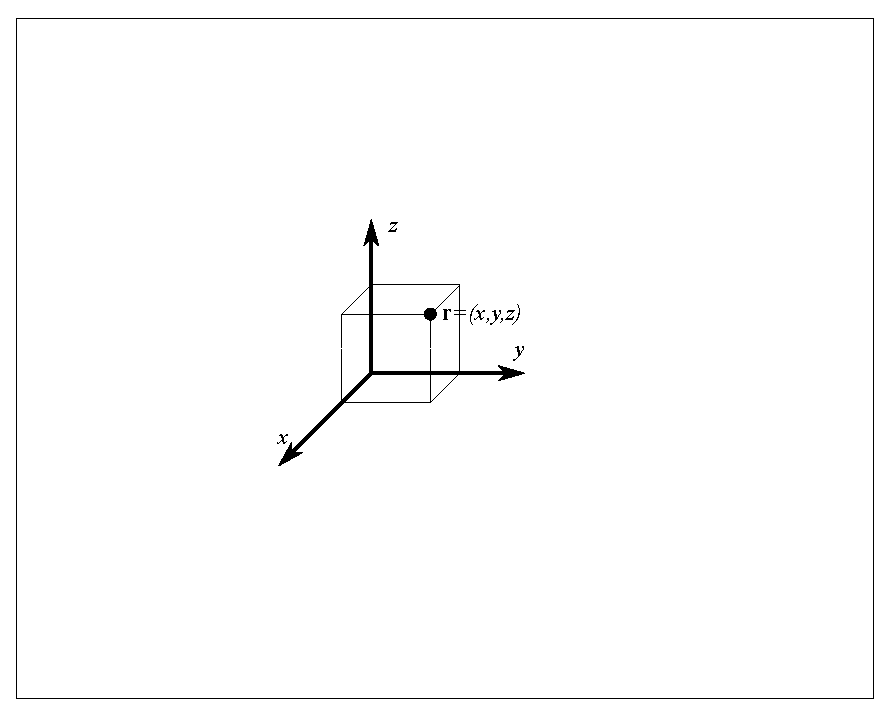
\includegraphics[width=0.8\textwidth]{figures/symmetry_planes_00.eps}
% \caption{Point in the reference octant}
% \end{figure}
% 
% \begin{figure}[p]
% \centering
% \includegraphics[width=0.8\textwidth]{figures/symmetry_planes_01.eps}
% \caption{Symmetric points with respect to plane $zx$}
% \end{figure}
% 
% \begin{figure}[p]
% \centering
% \includegraphics[width=0.8\textwidth]{figures/symmetry_planes_02.eps}
% \caption{Symmetric scalar field with respect to plane $zx$}
% \end{figure}
% 
% \begin{figure}[p]
% \centering
% \includegraphics[width=0.8\textwidth]{figures/symmetry_planes_03.eps}
% \caption{Symmetric vector field with respect to plane $zx$}
% \end{figure}
% 
% \begin{figure}[p]
% \centering
% \includegraphics[width=0.8\textwidth]{figures/symmetry_planes_04.eps}
% \caption{Symmetric rotation vector field with respect to plane $zx$}
% \end{figure}
% 
% \begin{figure}[p]
% \centering
% \includegraphics[width=0.8\textwidth]{figures/symmetry_planes_05.eps}
% \caption{Antisymmetric scalar field with respect to plane $zx$}
% \end{figure}
% 
% \begin{figure}[p]
% \centering
% \includegraphics[width=0.8\textwidth]{figures/symmetry_planes_06.eps}
% \caption{Antisymmetric vector field with respect to plane $zx$}
% \end{figure}
% 
% \begin{figure}[p]
% \centering
% \includegraphics[width=0.8\textwidth]{figures/symmetry_planes_07.eps}
% \caption{Antisymmetric rotation vector field with respect to plane $zx$}
% \end{figure}

\subsection{Section \texttt{conditions over be boundaries}}
In this section, the boundary conditions applied on the boundary elements boundaries are defined. All boundaries except the interfaces and the boundaries that are coupled with finite elements need to specify their boundary conditions. If not defined, a traction-free boundary is assumed by default. Here, boundary conditions for viscoelastic solids are explained.

There are available four boundary conditions for \textbf{ordinary boundaries}, two on global coordinates, and two in local coordinates, see Table \ref{tab:bc_ordinary_viscoelastic}. The two boundary conditions of each group are known displacement and known traction. For each boundary, the user must specify the boundary condition for each coordinate in local coordinates or in global coordinates, but not mixed.

\begin{table}
\centering
{\footnotesize
\begin{tabular}{crlll}
\textbf{Axes} & \textbf{Type} & \textbf{Name} & \textbf{Values} & \textbf{Equations} \\
\midrule
\multirow{4}{*}{global} & 0 & displacement & $U$ & $u_k=U$ \\
\cline{2-5}
                        & 1 & traction     & $T$ & $t_k=T$ \\
\cline{2-5}
                        & 4 & infinitesimal rotation field & center $\mathbf{c}$, axis $\mathbf{a}$, angle $\theta$ & $u_k=\theta\left[\mathbf{a}\times\left(\mathbf{x}-\mathbf{c}\right)\right]\cdot\mathbf{e}_k$ \\
\cline{2-5}
                        & 10 & normal pressure & $P$ & $t_k=Pn_k$ \\
\hline
\multirow{2}{*}{local}  & 2 & displacement & $U$ & $\mathbf{u}\cdot\mathbf{l}_k=U$ \\
\cline{2-5}
                        & 3 & traction     & $T$ & $\mathbf{t}\cdot\mathbf{l}_k=T$ \\
\midrule
\multicolumn{5}{l}{Note: $k=1,\ldots,n$ (global or local axes). Local axes are $\left\{\mathbf{l}_1,\mathbf{l}_2,\mathbf{l}_3\right\}=\left\{\mathbf{n},\mathbf{t}_1,\mathbf{t}_2\right\}$.} \\
\end{tabular}
}
\caption{Boundary conditions for ordinary boundaries}
\label{tab:bc_ordinary_viscoelastic}
\end{table}

It is always preferable using the B.C. expressed in global axes (B.C. 0 or 1) when possible because they do not need additional equations. If the boundary is planar and its normal vector is parallel to any global axis, then the B.C. expressed in local axes are not needed at all.

There are available two boundary conditions for each face of a \textbf{crack-like boundary}. One establishes a displacement, while the other establishes a traction, see Table \ref{tab:bc_crack_viscoelastic}.

\begin{table}
\centering
{\footnotesize
\begin{tabular}{crlll}
\textbf{Face} & \textbf{Type} & \textbf{Name} & \textbf{Values} & \textbf{Equations} \\
\midrule
\multirow{2}{*}{$\Gamma^+$} & 0 & displacement & $U^+$ & $u_k^+=U^+$ \\
\cline{2-5}
                            & 1 & traction     & $T^+$ & $t_k^+=T^+$ \\
\hline
\multirow{2}{*}{$\Gamma^-$} & 0 & displacement & $U^-$ & $u_k^-=U^-$ \\
\cline{2-5}
                            & 1 & traction     & $T^-$ & $t_k^-=T^-$ \\
\midrule
\multicolumn{5}{l}{Note: $k=1,\ldots,n$ (global axes).} \\
\end{tabular}
}
\caption{Boundary conditions for crack-like boundaries}
\label{tab:bc_crack_viscoelastic}
\end{table}

The general format of the section is:
\begin{Verbatim}[frame=single, fontsize=\small, label={general format of section [symmetry planes]}]
[conditions over be boundaries]
boundary <boundary id>: <type x> <value x>
                        <type y> <value y>
                        <type z> <value z>
                        <type x (if crack-like: face -)> <value x (if crack-like: face -)>
                        <type y (if crack-like: face -)> <value y (if crack-like: face -)>
                        <type z (if crack-like: face -)> <value z (if crack-like: face -)>
...
\end{Verbatim} 
where note that for two-dimensional problems, the $z$ lines must be removed. An example of a two-dimensional problem with two boundaries with identifiers \texttt{1} and \texttt{3}, being the first an ordinary boundary with null displacements and the second a crack-like boundary with traction-free faces:
\begin{Verbatim}[frame=single, fontsize=\small, label={input.dat}]
...

[conditions over be boundaries]
boundary 1: 0 0.
            0 0.
boundary 3: 1 0.
            1 0.
            1 0.
            1 0.
            
...
\end{Verbatim} 
The same example as before but for a three-dimensional problem:
\begin{Verbatim}[frame=single, fontsize=\small, label={input.dat}]
...

[conditions over be boundaries]
boundary 1: 0 0.
            0 0.
            0 0.
boundary 3: 1 0.
            1 0.
            1 0.
            1 0.
            1 0.
            1 0.
            
...
\end{Verbatim} 
Note that if the analysis is time harmonic, the values of the boundary conditions must be introduced as complex numbers, e.g.\texttt{(0.,0.)}.

\subsection{Section \texttt{conditions over nodes}}
In this section, the boundary conditions over nodes are applied. For nodes of boundary elements, this boundary condition over nodes overrides the boundary conditions applied over their boundaries, and the Tables \ref{tab:bc_ordinary_viscoelastic} and \ref{tab:bc_crack_viscoelastic} remains valid. For nodes of finite elements, the boundary conditions are applied to the displacements and the rotation, the type of boundary conditions are \texttt{0} for known displacement, and \texttt{1} for known force (or moment).

The general format for the section is similar to the conditions over boundaries:
\begin{Verbatim}[frame=single, fontsize=\small, label={general format of section [conditions over nodes]}]
[conditions over nodes]
node <node id>: <type x> <value x>
                <type y> <value y>
                <type z> <value z>
                <if fe: type for rot. x or alpha> <value for rot. x or alpha>
                <if fe: type for rot. y or beta>  <value for rot. y or beta>
                <if fe: type for rot. z>          <value for rotation z>
\end{Verbatim} 

For a two-dimensional problem, example of a clamped beam FE node with identifier \texttt{67}, and a pin beam FE node with identifier \texttt{41}: 
\begin{Verbatim}[frame=single, fontsize=\small, label={input.dat}]
...

[conditions over nodes]
node 67: 0 0.
         0 0.
         0 0.
node 41: 0 0.
         0 0.
         1 0.
\end{Verbatim} 

\subsection{Section \texttt{bem formulation over boundaries}}

In this section, the user can modify the BEM formulation, i.e. the type of Boundary Integral Equations (BIEs) to be used when building the BEM equations and the collocation strategy to be used. The default formulations (BIEs and collocation strategies) work for almost all cases, and any change done here should be done with care and only when necessary, see below. 

There are two fundamental types of BIEs used in MultiFEBE:
\begin{description}
    
    \item[Singular BIE (SBIE)] It is also called the displacement or pressure BIE, since this equation relates the primary field variable (displacements in elasticity, pressure in acoustics, ...) at the collocation point with the the primary and secondary (tractions in elasticity, fluxes, ...) field variables over the boundaries and the body loads. This BIE can be collocated everywhere (the collocation point is the location of the Dirac delta of the Green's function). However, the nodal collocation (collocation at the boundary element nodes) is the ideal since it leads to the best conditioning of the system. Non-nodal collocation is also possible, but it should be used only where nodal collocation turns problematic. 
    
    \item[Hypersingular BIE (HBIE)] It is also called the traction or flux BIE, since it relates the secondary field variable with the the primary and secondary field variables over the boundaries and body loads. This BIE can be collocated only where the discretization has $\mathcal{C}^1$ displacement continuity. Since MultiFEBE only considers $\mathcal{C}^0$ continuous elements, this means that HBIE must have non-nodal collocation (except at element interior nodes).
    
\end{description}

The non-nodal collocation strategy implemented here is the so-called Multiple Collocation Approach\footnote{J. Dom\'inguez \& M.P. Ariza. A direct traction BIE for three-dimensional
crack problems. Engng Anal Bound Elem 2000;24:727–38.} (MCA). When building the BIE associated with a given node, the MCA consists on building the equation by adding up as many BIEs as the number of elements sharing the node, being each BIE collocated near the node but shifted towards inside the element. For a given element, the local coordinates of the collocation point $(\xi^i_k,\eta^i_k)$ contributing to the node $k$ located at $(\xi_k,\eta_k)$ is controlled by the dimensionless distance $\delta$, which is a measure of the separation between the collocation point and the corresponding node such that:
\begin{align}
\textnormal{Line elements:}\quad\xi^i_k &= \left(1-\delta\right)\xi_k,\;\xi_k\in\left[-1,1\right] \\
\textnormal{Quadrilateral elements:}\quad\xi^i_k &= \left(1-\delta\right)\xi_k,\;\xi_k\in\left[-1,1\right] \\
\quad\eta^i_k &= \left(1-\delta\right)\eta_k,\;\eta_k\in\left[-1,1\right] \\
\textnormal{Triangular elements:}\quad\xi^i_k &= \left(1-\delta\right)\xi_k+\delta/3,\;\xi_k\in\left[0,1\right] \\
\quad\eta^i_k &= \left(1-\delta\right)\eta_k+\delta/3,\;\eta_k\in\left[0,1\right],\;\xi_k+\eta_k\leq1
\end{align}
This way $\delta\rightarrow0$ means that the collocation point is approaching the node, and $\delta\rightarrow1$ means that the collocation point is approaching the element's centroid in local coordinates. Formally $0<\delta<1$, but in practice it should be $0.01<\delta<0.6$. By default, we use is $\delta=0.42$ for linear elements, $\delta=0.23$ for quadratic elements and $\delta=0.14$ for cubic elements.

% Falta documentar la entrada via groups of nodes y parts. Falta implementar la entrada para opciones de formulacion de body loads.

\noindent The general format for this data section is:
\begin{Verbatim}[frame=single, fontsize=\small, label={general format of section [bem formulation over boundaries]}]
[bem formulation over boundaries]
boundary <boundary id>: <keyword: type of formulation> <values>
\end{Verbatim} 
\noindent where the available formulations and their options are given in Table~\ref{tab:bem_formulation_boundaries}. 

For instance, in a problem with six boundaries, where the collocation strategy in all boundaries must be nodal, with the exception of boundary 6, where a non-nodal collocation strategy is prefered for all the nodes along its boundaries, with a displacement towards inside each element of 10\% the width of the element, one should write:
\begin{Verbatim}[frame=single, fontsize=\small, label={input.dat}]
...

[bem formulation over boundaries]
boundary 1: sbie
boundary 2: sbie
boundary 3: sbie
boundary 4: sbie
boundary 5: sbie
boundary 6: sbie_boundary_mca 0.1
\end{Verbatim} 


\begin{table}
\centering
{\footnotesize
\begin{tabular}{lcL{10cm}}
\textbf{Keyword} & \textbf{Values} & \textbf{Description} \\
\midrule
\multicolumn{3}{c}{\textit{Ordinary boundaries}} \\
\midrule
\texttt{sbie} & none & SBIE with nodal collocation strategy for all nodes of the boundary. This is unsafe since at doubled nodes, depending on the boundary conditions, it can lead to a singular linear system of equations. \\
\texttt{sbie\_boundary\_mca} & $\delta$ & \textbf{This is the default formulation for ordinary boundaries.} SBIE with nodal collocation strategy for all nodes of the boundary except for the nodes at the boundary of the boundary, where MCA is used. The default value is $\delta=0.05$.  \\
\texttt{sbie\_mca} & $\delta$ & SBIE with MCA for all nodes of the boundary. The default value is indicated by Note 1. \\
\texttt{hbie} & $\delta$ & HBIE with MCA for all nodes. For using default values (see Note 1), the user must write a value $\delta\leq0$. Other values  \\
\texttt{dual\_bm\_same} & $\delta$ & Burton and Miller formulation (SBIE$+i/k$HBIE) for eliminating spurious frequencies when solving some exterior problems. SBIE and HBIE with MCA (same $\delta$) for all nodes. The default value is indicated by Note 1. \\
\texttt{dual\_bm\_mixed} & $\delta_\mathrm{S}$ $\delta_\mathrm{H}$ & Burton and Miller formulation (SBIE$+i/k$HBIE) for eliminating spurious frequencies when solving some exterior problems. SBIE with nodal collocation for all nodes of the boundary except for the nodes at the boundary of the boundary where MCA is used ($\delta_\mathrm{S}$), and HBIE with MCA ($\delta_\mathrm{H}$) for all nodes. For SBIE, the default value $\delta_\mathrm{S}=0.05$. For HBIE, the default value $\delta_\mathrm{H}$ is indicated by Note 1. \\
\midrule
\multicolumn{3}{c}{\textit{Crack-like boundaries}} \\
\midrule
\texttt{same} & $\delta$ & \textbf{This is the default formulation for crack-like boundaries.} Dual BEM (SBIE/HBIE) formulation for crack boundary elements with MCA for all nodes. The default value $\delta$ is indicated by Note 1. \\
\texttt{mixed} & $\delta_\mathrm{S}$ $\delta_\mathrm{H}$ & Dual BEM (SBIE/HBIE) formulation for crack boundary elements. SBIE with nodal collocation for all nodes of the boundary except for the nodes at the boundary of the boundary where MCA is used ($\delta_\mathrm{S}$), and HBIE with MCA ($\delta_\mathrm{H}$) for all nodes. For SBIE, the default value $\delta_\mathrm{S}=0.05$. For HBIE, the default value $\delta_\mathrm{H}$ is indicated by Note 1. \\
\end{tabular}
\begin{flushleft}
\begin{itemize}
\item General note 1: Formally $0<\delta<1$, but in practice it should be $0.01<\delta<0.6$.
\item General note 2: If the user assigns a value $\delta\leq0$, default values are considered.
\item Note 1: By default, $\delta=0.42$ for linear elements, $\delta=0.23$ for quadratic elements, and $\delta=0.14$ for cubic elements. 
\end{itemize}
\end{flushleft}



\caption{List of options and values in section \texttt{bem formulation boundaries}}
\label{tab:bem_formulation_boundaries}
}
\end{table}


\subsection{Section \texttt{incident waves}}
In this section, the incoming waves are defined. The incidence angles are shown in Figure \ref{fig:incidence}.

\begin{figure}[h]
\centering
%\include{figures/incidence_angle.eps_tex}
\includegraphics{figures/incidence_angle.pdf}
\caption{Incidence angles for two- and three-dimensional problems\label{fig:incidence}}
\end{figure}

The incident waves can be defined in terms of displacements (unitary displacements), in terms of stresses (unitary stresses) or in terms of the potentials (unitary potentials). The general format for the section is:
\begin{Verbatim}[frame=single, fontsize=\small, label={general format of section [incident waves]}]
[incident waves]
<number of incident waves>

<incident wave identifier>
<class: plane>
<space> [if space=half-space: <np> <xp> <bc>]
<variable> <amplitude> <x0(1)> <x0(2)> [if 3D: <x0(3)>] [if 3D: <varphi>] <theta>
<xs(1)> <xs(2)> [if 3D: <xs(3)>] <symconf(1)> <symconf(2)> [if 3D: <symconf(3)>]
<region_type> <wave_type>

...
\end{Verbatim} 
where angles have to be introduced in degrees.

Example of vertical P-wave in terms of displacements in the full-space: 
\begin{Verbatim}[frame=single, fontsize=\small, label={input.dat}]
...

[incident waves]
1
1
plane
full-space
0 1. 0. 0. 90.
0. 0. 0. 0.
viscoelastic p

...
\end{Verbatim} 
Example of vertical SV-wave in terms of displacements in the half-space: 
\begin{Verbatim}[frame=single, fontsize=\small, label={input.dat}]
...

[incident waves]
1
1
plane
half-space 2 0. 1
0 1. 0. 0. 90.
0. 0. 0. 0.
viscoelastic sv

...
\end{Verbatim}

% *********************************************************************************************
% *********************************************************************************************
% *********************************************************************************************

\chapter{Output files}

\label{ch:output_files}

\section{Introduction}

Output files are written according to the type of analysis and model, as well as the input file export section. By default the path and name of the output files is equal to the input file but with an additional extension. The path and name can be changed when calling the solver from the terminal as explained in \ref{sec:howto}. There are three main native output files with the following additional extensions: nodal solutions (\texttt{*.nso}), element solutions (\texttt{*.eso}) and stress resultant solutions (\texttt{*.tot}). The specific file format is different for static and time harmonic analysis. There is one Gmsh output file (\texttt{*.pos}) which contains the case mesh and results (MSH file format version 2.2).

\section{Nodal solutions file (\texttt{*.nso})}

% faltan puntos internos y cargas de volumen internas

This output file is a plain text file containing the nodal (node by node) results. The file starts with a set of header lines whose first character is ``\texttt{\#}'' (a comment line in GNU/Linux environments), describing the file and the meaning of the main data columns. The first 9 columns are always present, and indicates the following:
\begin{longtable}{ccp{11cm}}
\textbf{Column} & \textbf{Value} &\textbf{Description} \\ 
\endhead
\midrule
\$1 & integer & Analysis step index. For linear elastic static analysis it is always 0. For time harmonic analysis it is the frequency index. In future releases, it will receive the natural frequency index (for modal analysis), or the time step index (for transient analysis), or the loading step index (for non-linear static analysis). \\
\$2 & float & Analysis step value. For linear elastic static analysis it is always 0.0. For time harmonic analysis it is the frequency value (in Hz or rad/s depending on the units used in the frequencies section of the input file). In future releases, it will receive the natural frequency value (for modal analysis), or the time step value (for transient analysis), or the loading step value (for non-linear static analysis). \\
\$3 & integer & Identifier of the region to which the node result belongs. In the case of finite element nodes, this has no significance since results does not depend on the region. However, in the case of boundary elements belonging to two regions (interface boundary elements) this allows selecting which result is required. \\
\$4 & integer & Region class: 1 (BE region) or 2 (FE region). \\
\$5 & integer & Region type: 1 (inviscid fluid) or 2 (elastic solid) or 3 (poroelastic medium). \\
\$6 & integer & Identifier of the BE boundary (if \$4==1) or FE subregion (if \$4==2) to which the node result belongs. In the case of finite element nodes, this has no significance since results does not depend on the FE subregion. However, in the case of boundary elements belonging to two regions (interface boundary elements) this allows selecting which result is required. \\
\$7 & integer & If \$4==1, then it indicates the boundary class: 1 (ordinary) or 2 (crack-like). If \$4==2, then it indicates the number of degrees of freedom of the node. \\
\$8 & integer & If \$4==1, then it indicates the boundary face: 1 (positive normal) or 2 (negative normal). If \$4==2, then it is always 0. \\
\$9 & integer & Identifier of the node. \\
\end{longtable}
From column \$10 onwards, the meaning of each column differs depending on the problem dimension (2D or 3D), on the type of analysis (static or time harmonic), on the region class (BE or FE), on the region type (inviscid fluid, elastic solid, poroelastic medium), and on the number of DOF (if a FE region).

For 2D problems in a static analysis (all regions are only of the elastic solid type):
\begin{longtable}{ccp{11cm}}
\textbf{Column} & \textbf{Value} &\textbf{Description} \\ 
\endhead
\midrule
\$10,\$11 & float & Node $(x_1,x_2)$ coordinates. \\
\midrule
\multicolumn{3}{c}{BE region node}
\\
\$12,\$13 & float & Node displacements $(u_1,u_2)$. \\
\$14,\$15 & float & Node tractions $(t_1,t_2)$. \\
\midrule
\multicolumn{3}{c}{FE region node with 2 DOFs}
\\
\$12,\$13 & float & Node displacements $(u_1,u_2)$. \\
\$14,\$15 & float & Node forces $(f_1,f_2)$. \\
\midrule
\multicolumn{3}{c}{FE region node with 3 DOFs}
\\
\$12-\$14 & float & Node displacements/rotation $(u_1,u_2,\theta_3)$. \\
\$15-\$17 & float & Node forces/moment $(f_1,f_2,m_3)$. \\
\end{longtable}

For 3D problems in a static analysis (all regions are only of the elastic solid type):
\begin{longtable}{ccp{11cm}}
\textbf{Column} & \textbf{Value} &\textbf{Description} \\ 
\endhead
\midrule
\$10-\$12 & float & Node $(x_1,x_2,x_3)$ coordinates. \\
\midrule
\multicolumn{3}{c}{BE region node}
\\
\$13-\$15 & float & Node displacements $(u_1,u_2,u_3)$. \\
\$16-\$18 & float & Node tractions $(t_1,t_2,t_3)$. \\
\midrule
\multicolumn{3}{c}{FE region node with 3 DOFs}
\\
\$13-\$15 & float & Node displacements $(u_1,u_2,u_3)$. \\
\$16-\$18 & float & Node forces $(f_1,f_2,f_3)$. \\
\midrule
\multicolumn{3}{c}{FE region node with 5 DOFs (shell element nodes with local rotations)}
\\
\$13-\$17 & float & Node displacements/local rotations $(u_1,u_2,u_3,\alpha,\beta)$. \\
\$18-\$22 & float & Node forces/local moments $(f_1,f_2,f_3,m_\alpha,m_\beta)$. \\
\midrule
\multicolumn{3}{c}{FE region node with 6 DOFs}
\\
\$13-\$18 & float & Node displacements/rotations $(u_1,u_2,u_3,\theta_1,\theta_2,\theta_3)$. \\
\$19-\$24 & float & Node forces/moments $(f_1,f_2,f_3,m_1,m_2,m_3)$. \\
\end{longtable}

For 2D problems in a time harmonic analysis, where each node variable is written by two consecutive columns containing its real and imaginary parts (if \texttt{complex\_notation = cartesian} in \texttt{[export]} section) or absolute value and argument (if \texttt{complex\_notation = polar} in \texttt{[export]} section):
\begin{longtable}{ccp{11cm}}
\textbf{Column} & \textbf{Value} &\textbf{Description} \\ 
\endhead
\midrule
\$10,\$11 & float & Node $(x_1,x_2)$ coordinates. \\
\midrule
\multicolumn{3}{c}{BE region node (inviscid fluid)} \\
\$12,\$13 & float & Node pressure $p$ (total field). \\
\$14,\$15 & float & Node normal displacement $U_n$ (total field). \\
\$16,\$17 & float & Node pressure $p^\mathrm{inc}$ (incident field). \\
\$18,\$19 & float & Node normal displacement $U_n^\mathrm{inc}$ (incident field). \\
\$20-\$23 & float & Node displacement $(U_1,U_2)$ (total field). \\
\midrule
\multicolumn{3}{c}{BE region node (elastic solid)} \\
\$12-\$15 & float & Node displacements $(u_1,u_2)$ (total field). \\
\$16-\$19 & float & Node tractions $(t_1,t_2)$ (total field). \\
\$20-\$23 & float & Node displacements $(u_1^\mathrm{inc},u_2^\mathrm{inc})$ (incident field). \\
\$24-\$27 & float & Node tractions $(t_1^\mathrm{inc},t_2^\mathrm{inc})$ (incident field). \\
\midrule
\multicolumn{3}{c}{BE region node (poroelastic medium)} \\
\$12,\$13 & float & Node fluid equivalent pressure $\tau$ (total field). Note that it is related to the dynamic pore pressure by $\tau=-\phi p$, where $\phi$ is the porosity.\\
\$14-\$17 & float & Node solid displacements $(u_1,u_2)$ (total field). \\
\$18,\$19 & float & Node fluid normal displacement $U_n$ (total field). \\
\$20-\$23 & float & Node solid tractions $(t_1,t_2)$ (total field). \\
\$24,\$25 & float & Node fluid equivalent pressure $\tau^\mathrm{inc}$ (incident field).\\
\$26-\$29 & float & Node solid displacements $(u_1^\mathrm{inc},u_2^\mathrm{inc})$ (incident field). \\
\$30,\$31 & float & Node fluid normal displacement $U_n^\mathrm{inc}$ (incident field). \\
\$32-\$35 & float & Node solid tractions $(t_1^\mathrm{inc},t_2^\mathrm{inc})$ (incident field). \\
\$36-\$39 & float & Node fluid displacement $(U_1,U_2)$ (total field). \\
\midrule
\multicolumn{3}{c}{FE region node (only of elastic solid type) with 2 DOFs} \\
\$12-\$15 & float & Node displacements $(u_1,u_2)$. \\
\$16-\$19 & float & Node forces $(f_1,f_2)$. \\
\midrule
\multicolumn{3}{c}{FE region node (only of elastic solid type) with 3 DOFs} \\
\$12-\$17 & float & Node displacements/rotation $(u_1,u_2,\theta_3)$. \\
\$18-\$23 & float & Node forces/moment $(f_1,f_2,m_3)$. \\
\end{longtable}

For 3D problems in a time harmonic analysis, where as in the 2D case each node variable is written by two consecutive columns containing its real and imaginary parts (if \texttt{complex\_notation = cartesian} in \texttt{[export]} section) or absolute value and argument (if \texttt{complex\_notation = polar} in \texttt{[export]} section):
\begin{longtable}{ccp{11cm}}
\textbf{Column} & \textbf{Value} &\textbf{Description} \\ 
\midrule
\$10-\$12 & float & Node $(x_1,x_2,x_3)$ coordinates. \\
\midrule
\multicolumn{3}{c}{BE region node (inviscid fluid)} \\
\$13,\$14 & float & Node pressure $p$ (total field). \\
\$15,\$16 & float & Node normal displacement $U_n$ (total field). \\
\$17,\$18 & float & Node pressure $p^\mathrm{inc}$ (incident field). \\
\$19,\$20 & float & Node normal displacement $U_n^\mathrm{inc}$ (incident field). \\
\$21-\$24 & float & Node displacement $(U_1,U_2,U_3)$ (total field). \\
\midrule
\multicolumn{3}{c}{BE region node (elastic solid)} \\
\$13-\$18 & float & Node displacements $(u_1,u_2,u_3)$ (total field). \\
\$19-\$24 & float & Node tractions $(t_1,t_2,t_3)$ (total field). \\
\$25-\$30 & float & Node displacements $(u_1^\mathrm{inc},u_2^\mathrm{inc},u_3^\mathrm{inc})$ (incident field). \\
\$31-\$36 & float & Node tractions $(t_1^\mathrm{inc},t_2^\mathrm{inc},t_3^\mathrm{inc})$ (incident field). \\
\midrule
\multicolumn{3}{c}{BE region node (poroelastic medium)} \\
\$13,\$14 & float & Node fluid equivalent pressure $\tau$ (total field). Note that it is related to the dynamic pore pressure by $\tau=-\phi p$, where $\phi$ is the porosity.\\
\$15-\$20 & float & Node solid displacements $(u_1,u_2,u_3)$ (total field). \\
\$21,\$22 & float & Node fluid normal displacement $U_n$ (total field). \\
\$23-\$28 & float & Node solid tractions $(t_1,t_2,t_3)$ (total field). \\
\$29,\$30 & float & Node fluid equivalent pressure $\tau^\mathrm{inc}$ (incident field).\\
\$31-\$36 & float & Node solid displacements $(u_1^\mathrm{inc},u_2^\mathrm{inc},u_3^\mathrm{inc})$ (incident field). \\
\$37,\$38 & float & Node fluid normal displacement $U_n^\mathrm{inc}$ (incident field). \\
\$39-\$44 & float & Node solid tractions $(t_1^\mathrm{inc},t_2^\mathrm{inc},t_3^\mathrm{inc})$ (incident field). \\
\$45-\$50 & float & Node fluid displacement $(U_1,U_2,U_3)$ (total field). \\
\midrule
\multicolumn{3}{c}{FE region node (only of elastic solid type) with 3 DOFs} \\
\$13-\$18 & float & Node displacements $(u_1,u_2,u_3)$. \\
\$19-\$24 & float & Node forces $(f_1,f_2,f_3)$. \\
\midrule
\multicolumn{3}{c}{FE region node (only of elastic solid type) with 5 DOFs (shell element nodes with local rotations)}
\\
\$13-\$22 & float & Node displacements/local rotations $(u_1,u_2,u_3,\alpha,\beta)$. \\
\$23-\$32 & float & Node forces/local moments $(f_1,f_2,f_3,m_\alpha,m_\beta)$. \\
\midrule
\multicolumn{3}{c}{FE region node (only of elastic solid type) with 6 DOFs} \\
\$13-\$24 & float & Node displacements/rotation $(u_1,u_2,u_3,\theta_1,\theta_2,\theta_3)$. \\
\$25-\$36 & float & Node forces/moment $(f_1,f_2,f_3,m_1,m_2,m_3)$. \\
\end{longtable}

\section{Element solutions file (\texttt{*.eso})}

This output file is a plain text file containing the element (element node by element node) results (stress resultants on finite elements). In a future release, element by element stress resultants over each boundary element will also be included. The file starts with a set of header lines whose first character is ``\texttt{\#}'' (a comment line in GNU/Linux environments), describing the file and the meaning of the main data columns. The first 13 columns are always present, and indicates the following:
\begin{longtable}{ccp{11cm}}
\textbf{Column} & \textbf{Value} &\textbf{Description} \\ 
\endhead
\midrule
\$1 & integer & Analysis step index. For linear elastic static analysis it is always 0. For time harmonic analysis it is the frequency index. In future releases, it will receive the natural frequency index (for modal analysis), or the time step index (for transient analysis), or the loading step index (for non-linear static analysis). \\
\$2 & float & Analysis step value. For linear elastic static analysis it is always 0.0. For time harmonic analysis it is the frequency value (in Hz or rad/s depending on the units used in the frequencies section of the input file). In future releases, it will receive the natural frequency value (for modal analysis), or the time step value (for transient analysis), or the loading step value (for non-linear static analysis). \\
\$3 & integer & Identifier of the region to which the element node result belongs. In the case of finite element nodes, this has no significance since results does not depend on the region. However, in the case of boundary elements belonging to two regions (interface boundary elements) this allows selecting which result is required. \\
\$4 & integer & Region class: 1 (BE region) or 2 (FE region). \\
\$5 & integer & Region type: 1 (inviscid fluid) or 2 (elastic solid) or 3 (poroelastic medium). \\
\$6 & integer & Identifier of the BE boundary (if \$4==1) or FE subregion (if \$4==2) to which the element result belongs. In the case of boundary elements belonging to two regions (interface boundary elements) this allows selecting which result is required. \\
\$7 & integer & If \$4==1, then it indicates the boundary class: 1 (ordinary) or 2 (crack-like). If \$4==2, then it indicates the finite element dimension. \\
\$8 & integer & If \$4==1, then it indicates the boundary face: 1 (positive normal) or 2 (negative normal). If \$4==2, then it indicates the finite element type. \\
\$9-\$11 & integer & Element identifier, dimension and type. \\
\$12,\$13 & integer & Element node index and number of degrees of freedom. \\
\$14 & integer & Node identifier. \\
\end{longtable}

For 2D problems in a static analysis:
\begin{longtable}{ccp{11cm}}
\textbf{Column} & \textbf{Value} &\textbf{Description} \\ 
\endhead
\midrule
\$15,\$16 & float & Node $(x_1,x_2)$ coordinates. \\
\midrule
\multicolumn{3}{c}{Straight beam finite element} \\
\$17-\$19 & float & Axial force ($N_{x'}$), shear force ($V_{y'}$) and bending moment ($M_{z'}$). \\
\midrule
\multicolumn{3}{c}{Bar finite element} \\
\$17 & float & Axial force ($N_{x'}$). \\
\midrule
\multicolumn{3}{c}{Discrete translational spring finite element} \\
\$17,\$18 & float & Force on each spring: $N_{x'}$, $N_{y'}$. \\
\midrule
\multicolumn{3}{c}{Discrete translational/rotational spring finite element} \\
\$17-\$19 & float & Force/moment on each spring: $N_{x'}$, $N_{y'}$, $M_{z'}$.
\end{longtable}

For 3D problems in a static analysis:
\begin{longtable}{ccp{11cm}}
\textbf{Column} & \textbf{Value} &\textbf{Description} \\ 
\endhead
\midrule
\$15-\$17 & float & Node $(x_1,x_2,x_3)$ coordinates. \\
\midrule
\multicolumn{3}{c}{Straight beam finite element} \\
\$18-\$23 & float & Axial force ($N_{x'}$), shear forces ($V_{y'}$, $V_{z'}$), torsional moment ($M_{z'}$) and bending moments ($M_{y'}$, $M_{z'}$). \\
\midrule
\multicolumn{3}{c}{Bar finite element} \\
\$18 & float & Axial force ($N_{x'}$). \\
\midrule
\multicolumn{3}{c}{Discrete translational spring finite element} \\
\$18-\$20 & float & Force on each spring: $N_{x'}$, $N_{y'}$, $N_{z'}$. \\
\midrule
\multicolumn{3}{c}{Discrete translational/rotational spring finite element} \\
\$18-\$23 & float & Force/moment on each spring: $N_{x'}$, $N_{y'}$, $N_{z'}$, $M_{x'}$, $M_{y'}$, $M_{z'}$. \\
\midrule
\multicolumn{3}{c}{Discrete translational/rotational spring finite element} \\
\$18-\$25 & float & Membrane forces ($N_{x'}$, $N_{y'}$, $N_{x'y'}$), bending moments ($M_{x'}$, $M_{y'}$, $M_{x'y'}$) and shear forces ($V_{x'}$, $V_{y'}$).
\end{longtable}


For 2D problems in a time harmonic analysis, where each node variable is written by two consecutive columns containing its real and imaginary parts (if \texttt{complex\_notation = cartesian} in \texttt{[export]} section) or absolute value and argument (if \texttt{complex\_notation = polar} in \texttt{[export]} section):
\begin{longtable}{ccp{11cm}}
\textbf{Column} & \textbf{Value} &\textbf{Description} \\ 
\endhead
\midrule
\$15,\$16 & float & Node $(x_1,x_2)$ coordinates. \\
\midrule
\multicolumn{3}{c}{Straight beam finite element} \\
\$17-\$22 & float & Axial force ($N_{x'}$), shear force ($V_{y'}$) and bending moment ($M_{z'}$). \\
\midrule
\multicolumn{3}{c}{Bar finite element} \\
\$17,\$18 & float & Axial force ($N_{x'}$). \\
\midrule
\multicolumn{3}{c}{Discrete translational spring finite element} \\
\$17-\$20 & float & Force on each spring: $N_{x'}$, $N_{y'}$. \\
\midrule
\multicolumn{3}{c}{Discrete translational/rotational spring finite element} \\
\$17-\$22 & float & Force/moment on each spring: $N_{x'}$, $N_{y'}$, $M_{z'}$.
\end{longtable}

For 3D problems in a time harmonic analysis, where each node variable is written by two consecutive columns containing its real and imaginary parts (if \texttt{complex\_notation = cartesian} in \texttt{[export]} section) or absolute value and argument (if \texttt{complex\_notation = polar} in \texttt{[export]} section):
\begin{longtable}{ccp{11cm}}
\textbf{Column} & \textbf{Value} &\textbf{Description} \\ 
\endhead
\midrule
\$15-\$17 & float & Node $(x_1,x_2,x_3)$ coordinates. \\
\midrule
\multicolumn{3}{c}{Straight beam finite element} \\
\$18-\$29 & float & Axial force ($N_{x'}$), shear forces ($V_{y'}$, $V_{z'}$), torsional moment ($M_{z'}$) and bending moments ($M_{y'}$, $M_{z'}$). \\
\midrule
\multicolumn{3}{c}{Bar finite element} \\
\$18,\$19 & float & Axial force ($N_{x'}$). \\
\midrule
\multicolumn{3}{c}{Discrete translational spring finite element} \\
\$18-\$23 & float & Force on each spring: $N_{x'}$, $N_{y'}$, $N_{z'}$. \\
\midrule
\multicolumn{3}{c}{Discrete translational/rotational spring finite element} \\
\$18-\$29 & float & Force/moment on each spring: $N_{x'}$, $N_{y'}$, $N_{z'}$, $M_{x'}$, $M_{y'}$, $M_{z'}$. \\
\midrule
\multicolumn{3}{c}{Discrete translational/rotational spring finite element} \\
\$18-\$33 & float & Membrane forces ($N_{x'}$, $N_{y'}$, $N_{x'y'}$), bending moments ($M_{x'}$, $M_{y'}$, $M_{x'y'}$) and shear forces ($V_{x'}$, $V_{y'}$).
\end{longtable}

%\section{Resultant solutions file (\texttt{*.tot})}

\section{Gmsh results file (\texttt{*.pos})}

The Gmsh output file (\texttt{*.pos}) contains the case mesh and results (MSH file format version 2.2). It is a plain text containing all this data which can be read by Gmsh. The following set of results are exported to Gmsh:
\begin{itemize}
    \item Fluid pressure (positive faces). Only boundary elements.
    \item Fluid pressure (negative faces). Only boundary elements.
    \item Solid total displacements (positive faces). Boundary elements and finite elements.
    \item Solid total displacements (negative faces). Only boundary elements.
    \item Solid total tractions (positive faces). Only boundary elements.
    \item Solid total tractions (negative faces). Only boundary elements.
    \item FE nodal forces/reactions. Only finite elements.
    \item Beam stress resultants. Only finite elements.
    \item Beam stress resultants local axis $x'$, $y'$ and $z'$. Only finite elements.
    \item Bar stress resultants. Only finite elements.
    \item Shell stress resultants. Only finite elements.
    \item Shell stress resultants local axis $x'$, $y'$ and $z'$. Only finite elements.
\end{itemize}

%
% TEXTO DE MANUAL VIEJO Y OTROS...... FALTA ORGANIZAR Y ESCRIBIR COMO DIOS MANDA ......
%

% \section{Problem}
% 
% \section{Problem}
% 
% A mechanical problem can be:
% \begin{itemize}
%  \item \textbf{Two-dimensional ($n=2$).} A 2D mechanical problem can be:
%  \begin{itemize}
%   \item \textbf{Plain strain}
%   \item \textbf{Plain stress}
%  \end{itemize}
%  \item \textbf{Three-dimensional ($n=3$).}
% \end{itemize}
% 
% Two types of analysis can be carried out:
% \begin{itemize}
%  \item \texttt{static}
%  \item \texttt{time\_harmonic}
% \end{itemize}
% 
% \section{Model}
% 
% A model is composed by the following types of entities:
% \begin{itemize}
%   \item \textbf{Region}
%   \item \textbf{Boundary}
%   \item \textbf{Element}
%   \item \textbf{Node}
%   \item \textbf{Internal point}
%   \item \textbf{Incident field}
% \end{itemize}
% 
% \subsection{Region}
% 
% In a $n$-dimensional problem, a region (or sub-domain) $\Omega$ is a $n$-dimensional entity that is a part or the whole domain of the problem. A region must be associated with one of the following types of media:
% \begin{itemize}
%   \item \textbf{Inviscid fluid}
%   
%   \begin{tabular}{|clccl|}
%   \hline
%   \textbf{Id} & \textbf{Property} & \textbf{Symbol} & \textbf{Variable} & \textbf{Note} \\
%   \hline
%   1 & Bulk modulus             & $K$    & \texttt{K}   & - \\
%   2 & Density                  & $\rho$ & \texttt{rho} & - \\
%   3 & Hysteretic damping ratio & $\xi$  & \texttt{xi}  & - \\
%   \hline
%   \end{tabular}
%   
%   \item \textbf{Elastic solid} 
%   
%   \begin{tabular}{|clccl|}
%   \hline
%   \textbf{Id} & \textbf{Property} & \textbf{Symbol} & \textbf{Variable} & \textbf{Note} \\
%   \hline
%   1 & Young's modulus                           & $E$              & \texttt{E}      & * \\
%   2 & Poisson's ratio                           & $\nu$            & \texttt{nu}     & * \\
%   3 & Lam\'e's first parameter                  & $\lambda$        & \texttt{lambda} & * \\
%   4 & Lam\'e's second parameter (shear modulus) & $\mu$            & \texttt{mu}     & * \\
%   5 & Bulk modulus                              & $K$              & \texttt{K}      & * \\
%   6 & Density                                   & $\rho$           & \texttt{rho}    & - \\
%   7 & Hysteretic damping ratio                  & $\xi$            & \texttt{xi}     & - \\
%   \hline
%   \end{tabular}
%   
%   *Two of these properties must be defined.
%   
%   \item \textbf{Poroelastic solid}
%   
%   \begin{tabular}{|clccl|}
%   \hline
%   \textbf{Id} & \textbf{Property} & \textbf{Symbol} & \textbf{Variable} & \textbf{Note} \\
%   \hline
%   1  & Porosity                                  & $\phi$            & \texttt{phi}    & - \\
%   2  & Drained Young's modulus                   & $E$               & \texttt{E}      & * \\
%   3  & Drained Poisson's ratio                   & $\nu$             & \texttt{nu}     & * \\
%   4  & Drained Lam\'e's first parameter          & $\lambda$         & \texttt{lambda} & * \\
%   5  & Lam\'e's second parameter (shear modulus) & $\mu$             & \texttt{mu}     & * \\
%   6  & Bulk modulus                              & $K$               & \texttt{K}      & * \\
%   7  & Biot's coupling parameter $Q$             & $Q$               & \texttt{Q}      & - \\
%   8  & Biot's coupling parameter $R$            & $R$               & \texttt{R}      & - \\
%   9  & Fluid phase density                       & $\rho_\mathrm{f}$ & \texttt{rho\_f} & - \\
%   10 & Solid phase density                       & $\rho_\mathrm{s}$ & \texttt{rho\_s} & - \\
%   11 & Additional apparent density               & $\rho_\mathrm{a}$ & \texttt{rho\_a} & - \\
%   12 & Hysteretic damping ratio                  & $\xi$             & \texttt{xi}     & - \\
%   13 & Dissipation coefficient                   & $b$               & \texttt{b}      & - \\
%   \hline
%   \end{tabular}
%   
%   *Two of these properties must be defined.
%   
% \end{itemize}
% A region $\Omega$ can be discretized by two different methods:
% \begin{itemize}
%   \item \textbf{BEM (BE region).} The region is treated by the BEM. Its discretization is defined by its boundary $\partial\Omega$. A BE region must be a connected space. In other words, it is a piece of the whole domain of the problem.
%   \item \textbf{FEM (FE region).} The region is treated by the FEM (only for viscoelastic solids yet). Its discretization is defined by its FE elements. A FE region can be a disconnected space. In other words, it  lets to assign a material to a FE element.
% \end{itemize}
% The interaction between BE regions is done through their shared boundaries. The interaction between FE regions is done through their shared nodes. The interaction between BE regions and FE regions is done through the BE nodes and the FE nodes that shares the same position.
% 
% \subsection{Boundary}
% 
% In a $n$-dimensional problem, a boundary $\Gamma$ is a $(n-1)$-dimensional oriented entity that is a part or the whole boundary of BE regions. The whole boundary $\partial\Omega$ of a BE region $\Omega$ is defined as a set of boundaries:
% \begin{equation}
% \partial\Omega = \left\{\ldots,\Gamma_j,\ldots\right\}
% \end{equation}
% whose orientation must be outwards from the BE region. A minus sign before $\Gamma_j$ can be used to indicate the reversion of the orientation of $\Gamma_j$ in order to get a compatible $\partial\Omega$. There are two classes of boundaries:
% \begin{itemize}
%   \item \textbf{Ordinary.} An ordinary boundary is a boundary in the classical sense. It can be connected with one or two BE regions.
% 
%   \begin{minipage}[b]{\linewidth}
%     \centering
%     \begin{minipage}[t]{0.28\linewidth}
%       \begin{figure}[H]
%       \centering
%       \input{figures/ordinary_boundary_exterior.ps_tex}
%       \caption{Ordinary boundary connected with one region}
%       \end{figure}
%     \end{minipage}
%     \begin{minipage}[t]{0.71\linewidth}
%       \begin{figure}[H]
%       \centering
%       \input{figures/ordinary_boundary_interface.ps_tex}
%       \caption{Ordinary boundary connected with two regions}
%       \end{figure}
%     \end{minipage}
%   \end{minipage}
% 
%   \item \textbf{Crack-like.} A special boundary that lies inside a BE region and is composed by two sub-boundaries ($\Gamma^+$ and $\Gamma^-$) of opposite orientations but equal position. Thus, a crack-like boundary can be connected only with one BE region. Generally speaking, it is the condensed geometric description of a null thickness inclusion. Its orientation defines the orientation of the positive sub-boundary $\Gamma^+$, i.e. it defines which face is $\Gamma^+$ and which face is $\Gamma^-$.
%   
%   \begin{minipage}[b]{\linewidth}
%     \centering
%     \begin{figure}[H]
%       \centering
%       \input{figures/coincident_boundary.ps_tex}
%       \caption{Crack-like boundary}
%     \end{figure}
%   \end{minipage}
% \end{itemize}
% 
% Each boundary is build up with unique BE elements and nodes. The orientation of all the BE elements of a given boundary must be the same, which defines the orientation of the boundary itself. Each boundary can be coupled (all its BE element) with corresponding FE elements. 
% 
% \newpage
% 
% \subsubsection{Couplings}
% 
% A boundary allows one of the following types of coupling:
% \begin{itemize}
%   \item \textbf{Ordinary boundary}
%   \begin{itemize}
%     \item \textbf{BE.} The boundary is uncoupled.
%     \begin{itemize}
%       \item \textbf{BE(F)} (page \pageref{coupling:open_bef})
%       \item \textbf{BE(E)} (page \pageref{coupling:open_bee})
%       \item \textbf{BE(P)} (page \pageref{coupling:open_bep})
%     \end{itemize}
%     \item \textbf{BE-FE.} The boundary is coupled with a FE structural element.
%     \begin{itemize}
%       \item \textbf{BE(F)-FE}
%       \item \textbf{BE(E)-FE}
%       \item \textbf{BE(P)-FE}
%     \end{itemize}
%     \item \textbf{BE-BE.} The boundary couples two BE regions.
%     \begin{itemize}
%       \item \textbf{BE(F)-BE(F)} (page \pageref{coupling:open_bef_bef})
%       \item \textbf{BE(E)-BE(E)} (page \pageref{coupling:open_bee_bee})
%       \item \textbf{BE(P)-BE(P)} (page \pageref{coupling:open_bep_bep})
%       \item \textbf{BE(F)-BE(E)} (page \pageref{coupling:open_bef_bee})
%       \item \textbf{BE(F)-BE(P)} (page \pageref{coupling:open_bef_bep})
%       \item \textbf{BE(E)-BE(P)} (page \pageref{coupling:open_bee_bep})
%     \end{itemize}
%     \item \textbf{BE-FE-BE.} The boundary couples two BE regions through a FE structural element.
%     \begin{itemize}
%       \item \textbf{BE(F)-FE-BE(F)}
%       \item \textbf{BE(E)-FE-BE(E)}
%       \item \textbf{BE(P)-FE-BE(P)}
%       \item \textbf{BE(F)-FE-BE(E)}
%       \item \textbf{BE(F)-FE-BE(P)}
%       \item \textbf{BE(E)-FE-BE(P)}
%     \end{itemize}
%   \end{itemize}
%   \item \textbf{Crack-like boundary}
%   \begin{itemize}
%     \item \textbf{BE.} The boundary is uncoupled.
%     \begin{itemize}
%       \item \textbf{BE(F)} (page \pageref{coupling:cracklike_bef})
%       \item \textbf{BE(E)} (page \pageref{coupling:cracklike_bee})
%       \item \textbf{BE(P)} (page \pageref{coupling:cracklike_bep}) 
%     \end{itemize}
%     \item \textbf{BE-FE.} The boundary is coupled with a FE structural element.
%     \begin{itemize}
%       \item \textbf{BE(F)-FE}
%       \item \textbf{BE(E)-FE}
%       \item \textbf{BE(P)-FE}
%     \end{itemize}
%   \end{itemize}
% \end{itemize}
% where F stands for fluid, E stands for viscoelastic solid, and P stands for poroelastic solid. The variables and boundary conditions associated each case is detailed below.
% 
% \newpage
% 
% \paragraph{Ordinary boundary / BE(F)\label{coupling:open_bef}} Ordinary boundary of a fluid BE region.
% 
% \vspace{10pt}
% 
% \begin{tabular}{|rll|}
% \hline
% \multicolumn{3}{|c|}{\textbf{VARIABLES}} \\
% \hline
% \textbf{Number} & \textbf{Name} & \textbf{Variable} \\
% \hline
% 1 & pressure            & $p$  \\
% \hline
% 2 & normal displacement & $U_n$ \\
% \hline
% \end{tabular}
% 
% \vspace{10pt}
% 
% \begin{tabular}{|rlll|}
% \hline
% \multicolumn{4}{|c|}{\textbf{BOUNDARY CONDITIONS}} \\
% \hline
% \textbf{Type} & \textbf{Name} & \textbf{Values} & \textbf{Equations} \\
% \hline
% 0 & pressure                       & $P$     & $p=P$   \\
% \hline
% 1 & normal displacement            & $W$     & $U_n=W$ \\
% \hline
% 2 & Sommerfeld                     & -     & $U_n=\frac{i}{\rho c \omega}p$ \\
% \hline
% 3 & First-order Bayliss and Turkel & $R$   & $U_n=\left(\frac{i}{\rho c \omega}-\frac{1}{2R\rho\omega^2}\right)p$ \\
% \hline
% \end{tabular}
% 
% \newpage
% 
% \paragraph{Ordinary boundary / BE(E)\label{coupling:open_bee}} Ordinary boundary of a viscoelastic solid BE region.
% 
% \vspace{10pt}
% 
% \begin{tabular}{|rll|}
% \hline
% \multicolumn{3}{|c|}{\textbf{VARIABLES}} \\
% \hline
% \textbf{Number} & \textbf{Name} & \textbf{Variable} \\
% \hline
% $k$   & displacement & $u_k$ \\
% \hline
% $k+n$ & traction     & $t_k$ \\
% \hline
% \multicolumn{3}{|l|}{Note: $k=1,\ldots,n$ (global axes).} \\
% \hline
% \end{tabular}
% 
% \vspace{10pt}
% 
% \begin{tabular}{|c|rlll|}
% \hline
% \multicolumn{5}{|c|}{\textbf{BOUNDARY CONDITIONS}} \\
% \hline
% \textbf{Axes} & \textbf{Type} & \textbf{Name} & \textbf{Values} & \textbf{Equations} \\
% \hline
% \multirow{4}{*}{global} & 0 & displacement   & $U$ & $u_k=U$ \\
% \cline{2-5}
%                         & 1 & traction       & $T$ & $t_k=T$ \\
% \cline{2-5}
%                         & 4 & infinitesimal rotation field & center $\mathbf{c}$, axis $\mathbf{a}$, angle $\theta$ & $u_k=\theta\left[\mathbf{a}\times\left(\mathbf{x}-\mathbf{c}\right)\right]\cdot\mathbf{e}_k$ \\
% \cline{2-5}
%                         & 10 & normal pressure & $P$ & $t_k=Pn_k$ \\
% \hline
% \multirow{2}{*}{local}  & 2 & displacement & $U$ & $\mathbf{u}\cdot\mathbf{l}_k=U$ \\
% \cline{2-5}
%                         & 3 & traction     & $T$ & $\mathbf{t}\cdot\mathbf{l}_k=T$ \\
% \hline
% \multicolumn{5}{|l|}{Note: $k=1,\ldots,n$ (global or local axes). Local axes are $\left\{\mathbf{l}_1,\mathbf{l}_2,\mathbf{l}_3\right\}=\left\{\mathbf{n},\mathbf{t}_1,\mathbf{t}_2\right\}$.} \\
% \hline
% \end{tabular}
% 
% \vspace{10pt}
% 
% La condicion de contorno 4 solo se aplica a contornos BE y no a los nodos BE !!!!.
% 
% En los nodos FE, la condicion 4 tambien se mantiene para la rotacion infinitesimal, pero solo se mete a traves de un grupo !!!!!
% 
% It is preferable using the B.C. expressed in global axes (B.C. 0 or 1) when possible because they do not need additional equations. If the boundary is planar and its normal vector is parallel to any global axis, then the B.C. expressed in local axes are not needed at all.
% 
% \newpage
% 
% \paragraph{Ordinary boundary / BE(P)\label{coupling:open_bep}} Ordinary boundary of a poroelastic solid BE region.
% 
% \vspace{10pt}
% 
% \begin{tabular}{|rlll|}
% \hline
% \multicolumn{4}{|c|}{\textbf{VARIABLES}} \\
% \hline
% \textbf{Number} & \textbf{Phase} & \textbf{Name} & \textbf{Variable} \\
% \hline
% 0       & fluid & equivalent stress   & $\tau$ \\
% \hline
% $k$     & solid & displacement        & $u_k$  \\
% \hline
% $n+1$   & fluid & normal displacement & $U_n$  \\
% \hline
% $k+n+1$ & solid & traction            & $t_k$  \\
% \hline
% \multicolumn{4}{|l|}{Note: $k=1,\ldots,n$ (global axes).} \\
% \hline
% \end{tabular}
% 
% \vspace{10pt}
% 
% \begin{tabular}{|c|c|c|rlll|}
% \hline
% \multicolumn{7}{|c|}{\textbf{BOUNDARY CONDITIONS}} \\
% \hline
% \textbf{Phase} & \textbf{Pore} & \textbf{Axes} & \textbf{Type} & \textbf{Name} & \textbf{Values} & \textbf{Equations} \\
% \hline
% \multirow{3}{*}{fluid} & \multirow{2}{*}{open} & \multirow{2}{*}{-}      & 0 & equivalent pressure & $T$  & $\tau=T$ \\
% \cline{4-7}
%                        &                       &                         & 1 & normal displacement & $W$  & $U_n=W$  \\
% \cline{2-7}
%                        & close                 & -                       & 2 & impervious condition & none & $U_n=\mathbf{u}\cdot\mathbf{n}$ \\
% \hline
% \multirow{12}{*}{solid} & \multirow{6}{*}{open}  & \multirow{4}{*}{global} & 0 & displacement        & $U$  & $u_k=U$  \\
% \cline{4-7}
%                        &                        &                         & 1 & traction            & $T$  & $t_k=T$  \\
% \cline{4-7}
%                        &                         &                         & 8 & infinitesimal rotation field & center $\mathbf{c}$, axis $\mathbf{a}$, angle $\theta$ & $u_k=\theta\left[\mathbf{a}\times\left(\mathbf{x}-\mathbf{c}\right)\right]\cdot\mathbf{e}_k$ \\                       
% \cline{4-7}
%                        &                        &                         & 10 & normal pressure    & $P$  & $t_k=Pn_k$  \\
% \cline{3-7}
%                        &                        & \multirow{2}{*}{local}  & 2 & displacement        & $U$  & $\mathbf{u}\cdot\mathbf{l}_k=U$  \\
% \cline{4-7}
%                        &                        &                         & 3 & traction            & $T$  & $\mathbf{t}\cdot\mathbf{l}_k=T$  \\
% \cline{2-7}
%                        & \multirow{6}{*}{close} & \multirow{4}{*}{global} & 4 & displacement        & $U$  & $u_k=U$ \\
% \cline{4-7}
%                        &                         &                         & 40 & infinitesimal rotation field & center $\mathbf{c}$, axis $\mathbf{a}$, angle $\theta$ & $u_k=\theta\left[\mathbf{a}\times\left(\mathbf{x}-\mathbf{c}\right)\right]\cdot\mathbf{e}_k$ \\
% \cline{4-7}
%                        &                        &                         & 5 & total traction      & $T$  & $t_k+\tau n_k=T$ \\
% \cline{4-7}
%                        &                        &                         & 50 & total normal pressure & $P$  & $t_k+\tau n_k=Pn_k$ \\
% \cline{3-7}
%                        &                        & \multirow{2}{*}{local}  & 6 & displacement        & $U$  & $\mathbf{u}\cdot\mathbf{l}_k=U$ \\
% \cline{4-7}
%                        & & & 7 & total traction      & $T$  & $\mathbf{t}\cdot\mathbf{l}_k+\tau\mathbf{n}\cdot\mathbf{l}_k=T$ \\  
% \hline
% \multicolumn{7}{|l|}{Note: $k=1,\ldots,n$ (global or local axes). Local axes are $\left\{\mathbf{l}_1,\mathbf{l}_2,\mathbf{l}_3\right\}=\left\{\mathbf{n},\mathbf{t}_1,\mathbf{t}_2\right\}$.} \\
% \hline
% \end{tabular}
% 
% \vspace{10pt}
% 
% The implemented boundary conditions have been taken from \cite{skalak1963}.
% 
% \vspace{10pt}
% 
% \newpage
% 
% \paragraph{Crack-like boundary / BE(F)\label{coupling:cracklike_bef}} Crack-like boundary of a fluid BE region.
% 
% \vspace{10pt}
% 
% \begin{tabular}{|c|rll|}
% \hline
% \multicolumn{4}{|c|}{\textbf{VARIABLES}} \\
% \hline
% \textbf{Face} & \textbf{Number} & \textbf{Name} & \textbf{Variable} \\
% \hline
% \multirow{2}{*}{$\Gamma^+$} & 1 & pressure            & $p^+$    \\
% \cline{2-4}
%                             & 2 & normal displacement & $U_n^+$  \\
% \hline
% \multirow{2}{*}{$\Gamma^-$} & 1 & pressure            & $p^-$    \\
% \cline{2-4}
%                             & 2 & normal displacement & $U_n^-$  \\
% \hline
% \end{tabular}
% 
% \vspace{10pt}
% 
% \begin{tabular}{|c|rlll|}
% \hline
% \multicolumn{5}{|c|}{\textbf{BOUNDARY CONDITIONS}} \\
% \hline
% \textbf{Face} & \textbf{Type} & \textbf{Name} & \textbf{Values} & \textbf{Equations} \\
% \hline
% \multirow{2}{*}{$\Gamma^+$} & 0 & pressure            & $P^+$ & $p^+=P^+$   \\
% \cline{2-5}
%                             & 1 & normal displacement & $W^+$ & $U_n^+=W^+$ \\
% \hline
% \multirow{2}{*}{$\Gamma^-$} & 0 & pressure            & $P^-$ & $p^-=P^-$   \\
% \cline{2-5}
%                             & 1 & normal displacement & $W^-$ & $U_n^-=W^-$       \\
% \hline
% \end{tabular}
% 
% \vspace{10pt}
% 
% Implementation note: the sub-boundary $\Gamma^+$ is the face number 1, and $\Gamma^-$ is the face number 2.
% 
% \newpage
% 
% \paragraph{Crack-like boundary / BE(E)\label{coupling:cracklike_bee}} Crack-like boundary of a viscoelastic solid BE region.
% 
% \vspace{10pt}
% 
% \begin{tabular}{|c|rll|}
% \hline
% \multicolumn{4}{|c|}{\textbf{VARIABLES}} \\
% \hline
% \textbf{Face} & \textbf{Number} & \textbf{Name} & \textbf{Variable} \\
% \hline
% \multirow{2}{*}{$\Gamma^+$} & $k$   & displacement & $u_k^+$ \\
% \cline{2-4}
%                             & $k+n$ & traction     & $t_k^+$ \\
% \hline
% \multirow{2}{*}{$\Gamma^-$} & $k$   & displacement & $u_k^-$ \\
% \cline{2-4}
%                             & $k+n$ & traction     & $t_k^-$ \\
% \hline
% \multicolumn{4}{|l|}{Note: $k=1,\ldots,n$ (global axes).} \\
% \hline
% \end{tabular}
% 
% \vspace{10pt}
% 
% \begin{tabular}{|c|rlll|}
% \hline
% \multicolumn{5}{|c|}{\textbf{BOUNDARY CONDITIONS}} \\
% \hline
% \textbf{Face} & \textbf{Type} & \textbf{Name} & \textbf{Values} & \textbf{Equations} \\
% \hline
% \multirow{2}{*}{$\Gamma^+$} & 0 & displacement & $U^+$ & $u_k^+=U^+$ \\
% \cline{2-5}
%                             & 1 & traction     & $T^+$ & $t_k^+=T^+$ \\
% \cline{2-5}
%                         & 4 & infinitesimal rotation field & center $\mathbf{c}$, axis $\mathbf{a}$, angle $\theta$ & $u_k^+=\theta\left[\mathbf{a}\times\left(\mathbf{x}-\mathbf{c}\right)\right]\cdot\mathbf{e}_k$ \\
% \hline
% \multirow{2}{*}{$\Gamma^-$} & 0 & displacement & $U^-$ & $u_k^-=U^-$ \\
% \cline{2-5}
%                             & 1 & traction     & $T^-$ & $t_k^-=T^-$ \\
% \cline{2-5}
%                         & 4 & infinitesimal rotation field & center $\mathbf{c}$, axis $\mathbf{a}$, angle $\theta$ & $u_k^-=\theta\left[\mathbf{a}\times\left(\mathbf{x}-\mathbf{c}\right)\right]\cdot\mathbf{e}_k$ \\
% \hline
% \multicolumn{5}{|l|}{Note: $k=1,\ldots,n$ (global axes).} \\
% \hline
% \end{tabular}
% 
% \vspace{10pt}
% 
% Implementation note: the sub-boundary $\Gamma^+$ is the face number 1, and $\Gamma^-$ is the face number 2.
% 
% \newpage
% 
% \paragraph{Crack-like boundary / BE(P)\label{coupling:cracklike_bep}} Crack-like boundary of a poroelastic solid BE region.
% 
% \vspace{10pt}
% 
% \begin{tabular}{|c|rlll|}
% \hline
% \multicolumn{5}{|c|}{\textbf{VARIABLES}} \\
% \hline
% \textbf{Face} & \textbf{Number} & \textbf{Phase} & \textbf{Name} & \textbf{Variable} \\
% \hline
% \multirow{4}{*}{$\Gamma^+$} & 0       & fluid & equivalent stress   & $\tau^+$ \\
% \cline{2-5}
%                             & $k$     & solid & displacement        & $u_k^+$  \\
% \cline{2-5}
%                             & $n+1$   & fluid & normal displacement & $U_n^+$  \\
% \cline{2-5}
%                             & $k+n+1$ & solid & traction            & $t_k^+$  \\
% \hline
% \multirow{4}{*}{$\Gamma^-$} & 0       & fluid & equivalent stress   & $\tau^-$ \\
% \cline{2-5}
%                             & $k$     & solid & displacement        & $u_k^-$  \\
% \cline{2-5}
%                             & $n+1$   & fluid & normal displacement & $U_n^-$  \\
% \cline{2-5}
%                             & $k+n+1$ & solid & traction            & $t_k^-$  \\
% \hline
% \multicolumn{5}{|l|}{Note: $k=1,\ldots,n$ (global axes).} \\
% \hline
% \end{tabular}
% 
% \vspace{10pt}
% 
% \begin{minipage}{\textwidth}
% \begin{tabular}{|c|c|c|rlll|}
% \hline
% \multicolumn{7}{|c|}{\textbf{BOUNDARY CONDITIONS}} \\
% \hline
% \textbf{Face} & \textbf{Phase} & \textbf{Pore} & \textbf{Type} & \textbf{Name} & \textbf{Values} & \textbf{Equations} \\
% \hline
% \multirow{7}{*}{$\Gamma^+$} & \multirow{3}{*}{fluid} & \multirow{2}{*}{open}  & 0 & equivalent pressure  & $T^+$  & $\tau^+=T^+$ \\
% \cline{4-7}
%                             &                        &                        & 1 & normal displacement  & $U^+$  & $U_n^+=U^+$  \\
% \cline{3-7}
%                             &                        & close                  & 2 & impervious condition & none   & $U_n^+=\mathbf{u}^+\cdot\mathbf{n}^+$ \\
% \cline{2-7}
%                             & \multirow{4}{*}{solid} & \multirow{2}{*}{open}  & 0 & displacement        & $U^+$  & $u_k^+=U^+$  \\
% \cline{4-7}
%                             &                        &                        & 1 & traction            & $T^+$  & $t_k^+=T^+$  \\
% \cline{3-7}
%                             &                        & \multirow{2}{*}{close} & 2 & displacement        & $U^+$  & $u_k^+=U^+$  \\
% \cline{4-7}
%                             &                        &                        & 3 & total traction      & $T^+$  & $t_k^++\tau^+ n_k^+=T^+$ \\
% \hline
% \multirow{7}{*}{$\Gamma^-$} & \multirow{3}{*}{fluid} & \multirow{2}{*}{open}  & 0 & equivalent pressure  & $T^-$  & $\tau^-=T^-$ \\
% \cline{4-7}
%                             &                        &                        & 1 & normal displacement  & $U^-$  & $U_n^-=U^-$  \\
% \cline{3-7}
%                             &                        & close                  & 2 & impervious condition & none   & $U_n^-=\mathbf{u}^-\cdot\mathbf{n}^-$ \\
% \cline{2-7}
%                             & \multirow{4}{*}{solid} & \multirow{2}{*}{open}  & 0 & displacement        & $U^-$  & $u_k^-=U^-$  \\
% \cline{4-7}
%                             &                        &                        & 1 & traction            & $T^-$  & $t_k^-=T^-$  \\
% \cline{3-7}
%                             &                        & \multirow{2}{*}{close} & 2 & displacement        & $U^-$  & $u_k^-=U^-$  \\
% \cline{4-7}
%                             &                        &                        & 3 & total traction      & $T^-$  & $t_k^-+\tau^- n_k^-=T^-$ \\
% \hline
%  -                          & -                      & open                   & 4 & fluid-filled\footnote{Inviscid and incompressible} & none   & $\tau^+=\tau^-$ \\
%                             &                        &                        &   &                                       &        & 
% $\phi U_n^++(1-\phi)\mathbf{u}^+\cdot\mathbf{n}^+=-\phi U_n^--(1-\phi)\mathbf{u}^-\cdot\mathbf{n}^-$ \\
%                             &                        &                        &   &               &        & $\mathbf{t}^+=(1/\phi-1)\tau^+\mathbf{n}^+$ \\ 
%                             &                        &                        &   &               &        & $\mathbf{t}^-=(1/\phi-1)\tau^-\mathbf{n}^-$ \\                
% \hline
%  -                          & -                      & close                  & 5 & fluid-filled & none   & 
%  $U_n^+=\mathbf{u}^+\cdot\mathbf{n}^+$, $U_n^-=\mathbf{u}^-\cdot\mathbf{n}^-$ \\
%                             &                        &                        &   &                                                    &        & 
%  $(\mathbf{u}^--\mathbf{u}^+)\cdot\mathbf{n}^+=0$  \\
%                             &                        &                        &   &                                                    &        & 
%  $\tau^+\mathbf{n}^++\mathbf{t}^++\tau^-\mathbf{n}^-+\mathbf{t}^-=\mathbf{0}$ \\
%                             &                        &                        &   &                                                    &        & 
%  $\mathbf{t}^+\cdot\mathbf{t}_j^+=0,j=1,n-1$ \\
% \hline
% \multicolumn{7}{|l|}{Note: $k=1,\ldots,n$ (global or local axes). Local axes are $\left\{\mathbf{l}_1,\mathbf{l}_2,\mathbf{l}_3\right\}=\left\{\mathbf{n},\mathbf{t}_1,\mathbf{t}_2\right\}$.} \\
% \hline
% \end{tabular}
% \end{minipage}
% 
% Fluid-filled crack: in fluid phase write b.c. type 3, and in solid phase b.c. type 4, it must be done for each face.......
% 
% \vspace{10pt}
% 
% Implementation note: the sub-boundary $\Gamma^+$ is the face number 1, and $\Gamma^-$ is the face number 2.
% The implemented boundary conditions have been taken from \cite{skalak1963}.
% 
% \newpage
% 
% \paragraph{Ordinary boundary / BE(F)-BE(F)\label{coupling:open_bef_bef}} Ordinary boundary that interconnects two fluid BE regions. In the local numbering of the boundary, the region 1 is the region where the boundary has positive orientation, and the region 2 is the region where the boundary has negative orientation.
% 
% \vspace{10pt}
% 
% \begin{tabular}{|c|rll|}
% \hline
% \multicolumn{4}{|c|}{\textbf{VARIABLES}} \\
% \hline
% \textbf{Region} & \textbf{Number} & \textbf{Name} & \textbf{Variable}  \\
% \hline
% \multirow{2}{*}{1} & 1 & pressure            & $p^{(1)}$    \\
% \cline{2-4}
%                    & 2 & normal displacement & $U_n^{(1)}$  \\
% \hline
% \multirow{2}{*}{2} & 1 & pressure            & $p^{(2)}$    \\
% \cline{2-4}
%                    & 2 & normal displacement & $U_n^{(2)}$  \\
% \hline
% \end{tabular}
% 
% \vspace{10pt}
% 
% \begin{tabular}{|r|lll|}
% \hline
% \multicolumn{4}{|c|}{\textbf{BOUNDARY CONDITIONS}}  \\
% \hline
% \textbf{Type} & \textbf{Name} & \textbf{Values} & \textbf{Equations} \\
% \hline
% (default) 0 & perfect bonding & none & $p^{(1)}=p^{(2)}$       \\
%             &                 &      & $U_n^{(1)}=-U_n^{(2)}$ \\
% \hline
% \end{tabular}
% 
% \newpage
% 
% \paragraph{Ordinary boundary / BE(E)-BE(E)\label{coupling:open_bee_bee}} Ordinary boundary that interconnects two viscoelastic solid BE regions. In the local numbering of the boundary, the region 1 is the region where the boundary has positive orientation, and the region 2 is the region where the boundary has negative orientation.
% 
% \vspace{10pt}
% 
% \begin{tabular}{|c|rll|}
% \hline
% \multicolumn{4}{|c|}{\textbf{VARIABLES}} \\
% \hline
% \textbf{Region} & \textbf{Number} & \textbf{Name} & \textbf{Variable}  \\
% \hline
% \multirow{2}{*}{1} & $k$   & displacement & $u_k^{(1)}$  \\
% \cline{2-4}
%                    & $k+n$ & traction     & $t_k^{(1)}$  \\
% \hline
% \multirow{2}{*}{2} & $k$   & displacement & $u_k^{(2)}$  \\
% \cline{2-4}
%                    & $k+n$ & traction     & $t_k^{(2)}$  \\
% \hline
% \multicolumn{4}{|l|}{Note: $k=1,\ldots,n$ (global axes).} \\
% \hline
% \end{tabular}
% 
% \vspace{10pt}
% 
% \begin{tabular}{|c|rlll|}
% \hline
% \multicolumn{5}{|c|}{\textbf{BOUNDARY CONDITIONS}}  \\
% \hline
% \textbf{Axes} & \textbf{Number} & \textbf{Name} & \textbf{Values} & \textbf{Equations} \\
% \hline
% \multirow{6}{*}{global} & (default) 0 & perfect bonding   & none          & $t_k^{(1)}+t_k^{(2)}=0$                                                         \\
%                         &             &                   &               & $u_k^{(1)}=u_k^{(2)}$                                                           \\
% \cline{2-5}
%                         & 1           & perfect debonding & none          & $t_k^{(1)}=0$                                                                   \\
%                         &             &                   &               & $t_k^{(2)}=0$                                                                   \\
% \cline{2-5}
%                         & 2           & partial bonding   & $K$, $C$, $M$ & $t_k^{(1)}+t_k^{(2)}=0$                                                         \\
%                         &             &                   &               & $\left(u_k^{(2)}-u_k^{(1)}\right)\left(K+i\omega C-\omega^2 M\right)=t_k^{(1)}$ \\
% \hline
% \multirow{6}{*}{local}  & 3           & perfect bonding   & none          & $t_k^{(1)}+t_k^{(2)}=0$                                                   \\
%                         &             &                   &               & $\left(\mathbf{u}^{(2)}-\mathbf{u}^{(1)}\right)\cdot\mathbf{l}_k^{(1)}=0$ \\
% \cline{2-5}
%                         & 4           & perfect debonding & none          & $t_k^{(1)}+t_k^{(2)}=0$                                                   \\
%                         &             &                   &               & $\mathbf{t}^{(1)}\cdot\mathbf{l}_k^{(1)}=0$                               \\
% \cline{2-5}
%                         & 5           & partial bonding   & $K$, $C$, $M$ & $t_k^{(1)}+t_k^{(2)}=0$                                                   \\
%                         &             &                   &               & $\left(\mathbf{u}^{(2)}-\mathbf{u}^{(1)}\right)\cdot\mathbf{l}_k^{(1)}\left(K+i\omega C-\omega^2 M\right)=\mathbf{t}^{(1)}\cdot\mathbf{l}_k^{(1)}$ \\
% \hline
% \multicolumn{5}{|l|}{Note: $k=1,\ldots,n$ (global or local axes). Local axes are $\left\{\mathbf{l}_1,\mathbf{l}_2,\mathbf{l}_3\right\}=\left\{\mathbf{n},\mathbf{t}_1,\mathbf{t}_2\right\}$.} \\
% \hline
% \end{tabular}
% 
% \vspace{10pt}
% 
% These boundary conditions are based on the concepts exposed in \cite{schoenberg1980}. It is preferable using the B.C. expressed in global axes (B.C. 0, 1 or 2) when possible because they do not need additional equations. If the boundary is planar and its normal vector is parallel to a global axis, then the B.C. expressed in local axes are not needed at all. Also, if a boundary connects two regions that are perfectly welded in all directions, then use the B.C. 0 for all $k$, whether or not the boundary is planar, whether or not its normal vector is parallel to a global axis. This last situation is the most common.
% 
% \newpage
% 
% \paragraph{Ordinary boundary / BE(F)-BE(E)\label{coupling:open_bef_bee}} Ordinary boundary that interconnects a fluid BE region and a viscoelastic solid (impermeable) BE region.
% 
% \vspace{10pt}
% 
% \begin{tabular}{|c|rll|}
% \hline
% \multicolumn{4}{|c|}{\textbf{VARIABLES}} \\
% \hline
% \textbf{Region} & \textbf{Number} & \textbf{Name} & \textbf{Variable} \\
% \hline
% \multirow{2}{*}{F} & 1     & pressure            & $p^{(F)}$   \\
% \cline{2-4}
%                    & 2     & normal displacement & $U_n^{(F)}$ \\
% \hline
% \multirow{2}{*}{E} & $k$   & displacement        & $u_k^{(E)}$ \\
% \cline{2-4}
%                    & $k+n$ & traction            & $t_k^{(E)}$ \\
% \hline
% \multicolumn{4}{|l|}{Note: $k=1,\ldots,n$ (global axes).} \\
% \hline
% \end{tabular}
% 
% \vspace{10pt}
% 
% \begin{tabular}{|rlll|}
% \hline
% \multicolumn{4}{|c|}{\textbf{BOUNDARY CONDITIONS}}  \\
% \hline
% \textbf{Number} & \textbf{Name} & \textbf{Values} & \textbf{Equations} \\
% \hline
% (default) 0 & perfect bonding & none & $-p^{(F)}\mathbf{n}^{(F)}+\mathbf{t}^{(E)}=\mathbf{0}$ \\
%             &                 &      & $U_n^{(F)}=-\mathbf{u}^{(E)}\cdot\mathbf{n}^{(E)}$     \\
% \hline
% \end{tabular}
% 
% \vspace{10pt}
% 
% In the local numbering of the boundary, the region 1 is the region where the boundary has positive orientation, and the region 2 is the region where the boundary has negative orientation. Thus, two cases must be implemented: $(F=1,E=2)$, and $(F=2,E=1)$.
% 
% \newpage
% 
% \paragraph{Ordinary boundary / BE(P)-BE(P)\label{coupling:open_bep_bep}} Ordinary boundary that interconnects two poroelastic solid BE regions. In the local numbering of the boundary, the region 1 is the region where the boundary has positive orientation, and the region 2 is the region where the boundary has negative orientation.
% 
% 
% \vspace{10pt}
% 
% \begin{tabular}{|c|rlll|}
% \hline
% \multicolumn{5}{|c|}{\textbf{VARIABLES}} \\
% \hline
% \textbf{Region} & \textbf{Number} & \textbf{Phase} & \textbf{Name} & \textbf{Variable}  \\
% \hline
% \multirow{4}{*}{1} & 0       & fluid & equivalent stress   & $\tau^{(1)}$ \\
% \cline{2-5}
%                    & $k$     & solid & displacement        & $u_k^{(1)}$  \\
% \cline{2-5}
%                    & $n+1$   & fluid & normal displacement & $U_n^{(1)}$  \\
% \cline{2-5}
%                    & $k+n+1$ & solid & traction            & $t_k^{(1)}$  \\
% \hline
% \multirow{4}{*}{2} & 0       & fluid & equivalent stress   & $\tau^{(2)}$ \\
% \cline{2-5}
%                    & $k$     & solid & displacement        & $u_k^{(2)}$  \\
% \cline{2-5}
%                    & $n+1$   & fluid & normal displacement & $U_n^{(2)}$  \\
% \cline{2-5}
%                    & $k+n+1$ & solid & traction            & $t_k^{(2)}$  \\
% \hline
% \multicolumn{5}{|l|}{Note: $k=1,\ldots,n$ (global axes).} \\
% \hline
% \end{tabular}
% 
% \vspace{10pt}
% 
% \begin{tabular}{|rlll|}
% \hline
% \multicolumn{4}{|c|}{\textbf{BOUNDARY CONDITIONS}}  \\
% \hline
% \textbf{Number} & \textbf{Name} & \textbf{Values} & \textbf{Equations} \\
% \hline
% (default) 0 & perfectly permeable   & none & $\mathbf{t}^{(1)}+\tau^{(1)}\mathbf{n}^{(1)}+\mathbf{t}^{(2)}+\tau^{(2)}\mathbf{n}^{(2)}=\mathbf{0}$ \\
%             &                       &      & $\mathbf{u}^{(1)}=\mathbf{u}^{(2)}$                                                                  \\
%             &                       &      & $\tau^{(1)}/\phi^{(1)}=\tau^{(2)}/\phi^{(2)}$                                                        \\
%             &                       &      & $\phi^{(1)}\left(U_n^{(1)}-\mathbf{u}^{(1)}\cdot\mathbf{n}^{(1)}\right)=-\phi^{(2)}\left(U_n^{(2)}-\mathbf{u}^{(2)}\cdot\mathbf{n}^{(2)}\right)$ \\
% \hline
%           1 & perfectly impermeable & none & $\mathbf{t}^{(1)}+\tau^{(1)}\mathbf{n}^{(1)}+\mathbf{t}^{(2)}+\tau^{(2)}\mathbf{n}^{(2)}=\mathbf{0}$ \\
%             &                       &      & $\mathbf{u}^{(1)}=\mathbf{u}^{(2)}$                                                                  \\
%             &                       &      & $U_n^{(1)}=\mathbf{u}^{(1)}\cdot\mathbf{n}^{(1)}$                                                    \\
%             &                       &      & $U_n^{(2)}=\mathbf{u}^{(2)}\cdot\mathbf{n}^{(2)}$                                                    \\
% \hline
%           2 & partially permeable   & $k\;\mathrm{[N \cdot s \cdot m^{-3}]}$ & $\mathbf{t}^{(1)}+\tau^{(1)}\mathbf{n}^{(1)}+\mathbf{t}^{(2)}+\tau^{(2)}\mathbf{n}^{(2)}=\mathbf{0}$ \\
%             &                       &      & $\mathbf{u}^{(1)}=\mathbf{u}^{(2)}$                                                                  \\
%             &                       &      & $-\tau^{(1)}/\phi^{(1)}+\tau^{(2)}/\phi^{(2)} = i \omega k \phi^{(1)}(U_n^{(1)}-\mathbf{u}^{(1)}\cdot\mathbf{n}^{(1)})$                                                        \\
%             &                       &      & $\phi^{(1)}\left(U_n^{(1)}-\mathbf{u}^{(1)}\cdot\mathbf{n}^{(1)}\right)=-\phi^{(2)}\left(U_n^{(2)}-\mathbf{u}^{(2)}\cdot\mathbf{n}^{(2)}\right)$
%             \\
% \hline
% \end{tabular}
% 
% \newpage
% 
% \paragraph{Ordinary boundary / BE(F)-BE(P)\label{coupling:open_bef_bep}} Ordinary boundary that interconnects a fluid BE region and a poroelastic solid BE region.
% 
% \vspace{10pt}
% 
% \begin{tabular}{|c|rcll|}
% \hline
% \multicolumn{5}{|c|}{\textbf{VARIABLES}} \\
% \hline
% \textbf{Region} & \textbf{Number} & \textbf{Phase} & \textbf{Name} & \textbf{Variable} \\
% \hline
% \multirow{2}{*}{F} & 1       &       & pressure            & $p^{(F)}$     \\
% \cline{2-5}
%                    & 2       &       & normal displacement & $U_n^{(F)}$   \\
% \hline
% \multirow{4}{*}{P} & 0       & fluid & equivalent stress   & $\tau^{(P)}$  \\
% \cline{2-5}
%                    & $k$     & solid & displacement        & $u_k^{(P)}$   \\
% \cline{2-5}
%                    & $n+1$   & fluid & normal displacement & $U_n^{(P)}$   \\
% \cline{2-5}
%                    & $k+n+1$ & solid & traction            & $t_k^{(P)}$   \\
% \hline
% \multicolumn{5}{|l|}{Note: $k=1,\ldots,n$ (global axes).} \\
% \hline
% \end{tabular}
% 
% \vspace{10pt}
% 
% \begin{tabular}{|rlll|}
% \hline
% \multicolumn{4}{|c|}{\textbf{BOUNDARY CONDITIONS}}  \\
% \hline
% \textbf{Number} & \textbf{Name} & \textbf{Values} & \textbf{Equations} \\
% \hline
% (default) 0 & perfectly permeable & none & $-\left(1-\phi^{(P)}\right)p^{(F)}\mathbf{n}^{(F)}+\mathbf{t}^{(P)}=\mathbf{0}$                 \\ % Equilibrio (esqueleto solido): n ecuaciones
%             &                     &      & $p^{(F)}=-\tau^{(P)}/\phi^{(P)}$                                                                \\ % Equilibrio (fase fluida): 1 ecuacion
%             &                     &      & $U_n^{(F)}=-\phi^{(P)}U_n^{(P)}-\left(1-\phi^{(P)}\right)\mathbf{u}^{(P)}\cdot\mathbf{n}^{(P)}$ \\ % Compatibilidad: 1 ecuacion
% \hline
%           1 & perfectly impermeable & none & $-p^{(F)}\mathbf{n}^{(F)}+\mathbf{t}^{(P)}+\tau^{(P)}\mathbf{n}^{(P)}=\mathbf{0}$  \\ % Equilibrio (medio homogeneo): n ecuaciones
%             &                       &      & $U_n^{(P)}=\mathbf{u}^{(P)}\cdot\mathbf{n}^{(P)}$                                  \\ % Condicion de impermeabilidad: 1 ecuacion
%             &                       &      & $U_n^{(F)}=-U_n^{(P)}$                                                             \\ % Compatibilidad: 1 ecuacion  
% \hline
% \end{tabular}
% 
% \vspace{10pt}
% 
% In the local numbering of the boundary, the region 1 is the region where the boundary has positive orientation, and the region 2 is the region where the boundary has negative orientation. Thus, two cases must be implemented: $(F=1,P=2)$, and $(F=2,P=1)$.
% 
% \newpage
% 
% \paragraph{Ordinary boundary / BE(E)-BE(P)\label{coupling:open_bee_bep}} Ordinary boundary that interconnects a viscoelastic solid (impermeable) BE region and a poroelastic solid BE region.
% 
% \vspace{10pt}
% 
% \begin{tabular}{|c|rcll|}
% \hline
% \multicolumn{5}{|c|}{\textbf{VARIABLES}} \\
% \hline
% \textbf{Region} & \textbf{Number} & \textbf{Phase} & \textbf{Name} & \textbf{Variable} \\
% \hline
% \multirow{2}{*}{E} & $k$     &       & displacement        & $u_k^{(E)}$  \\
% \cline{2-5}
%                    & $k+n$   &       & traction            & $t_k^{(E)}$  \\
% \hline
% \multirow{4}{*}{P} & 0       & fluid & equivalent stress   & $\tau^{(P)}$ \\
% \cline{2-5}
%                    & $k$     & solid & displacement        & $u_k^{(P)}$  \\
% \cline{2-5}
%                    & $n+1$   & fluid & normal displacement & $U_n^{(P)}=\mathbf{u}^{(P)}\cdot\mathbf{n}^{(P)}$ (impermeable condition)  \\
% \cline{2-5}
%                    & $k+n+1$ & solid & traction            & $t_k^{(P)}$  \\
% \hline
% \multicolumn{5}{|l|}{Note: $k=1,\ldots,n$ (global axes).} \\
% \hline
% \end{tabular}
% 
% \vspace{10pt}
% 
% \begin{tabular}{|c|rlll|}
% \hline
% \multicolumn{5}{|c|}{\textbf{BOUNDARY CONDITIONS}}  \\
% \hline
% \textbf{Axes} & \textbf{Number} & \textbf{Name} & \textbf{Values} & \textbf{Equations} \\
% \hline
% \multirow{6}{*}{global} & (default) 0 & perfect bonding   & none          & $t_k^{(E)}+\tau^{(P)}n_k^{(P)}+t_k^{(P)}=0$                                     \\
%                         &             &                   &               & $u_k^{(E)}=u_k^{(P)}$                                                           \\
% \cline{2-5}
%                         & 1           & perfect debonding & none          & $t_k^{(E)}=0$                                                                   \\
%                         &             &                   &               & $\tau^{(P)}n_k^{(P)}+t_k^{(P)}=0$                                               \\
% \cline{2-5}
%                         & 2           & partial bonding   & $K$, $C$, $M$ & $t_k^{(E)}+\tau^{(P)}n_k^{(P)}+t_k^{(P)}=0$                                     \\
%                         &             &                   &               & $\left(u_k^{(P)}-u_k^{(E)}\right)\left(K+i\omega C-\omega^2 M\right)=t_k^{(E)}$ \\
% \hline
% \multirow{6}{*}{local}  & 3           & perfect bonding   & none          & $t_k^{(E)}+\tau^{(P)}n_k^{(P)}+t_k^{(P)}=0$                               \\
%                         &             &                   &               & $\left(\mathbf{u}^{(P)}-\mathbf{u}^{(E)}\right)\cdot\mathbf{l}_k^{(E)}=0$ \\
% \cline{2-5}
%                         & 4           & perfect debonding & none          & $t_k^{(E)}+\tau^{(P)}n_k^{(P)}+t_k^{(P)}=0$                               \\
%                         &             &                   &               & $\mathbf{t}^{(E)}\cdot\mathbf{l}_k^{(E)}=0$                               \\
% \cline{2-5}
%                         & 5           & partial bonding   & $K$, $C$, $M$ & $t_k^{(E)}+\tau^{(P)}n_k^{(P)}+t_k^{(P)}=0$                               \\
%  & & & & $\left(\mathbf{u}^{(P)}-\mathbf{u}^{(E)}\right)\cdot\mathbf{l}_k^{(E)}\left(K+i\omega C-\omega^2 M\right)=\mathbf{t}^{(E)}\cdot\mathbf{l}_k^{(E)}$ \\
% \hline
% \multicolumn{5}{|l|}{Note: $k=1,\ldots,n$ (global or local axes). Local axes are $\left\{\mathbf{l}_1,\mathbf{l}_2,\mathbf{l}_3\right\}=\left\{\mathbf{n},\mathbf{t}_1,\mathbf{t}_2\right\}$.} \\
% \hline
% \end{tabular}
% 
% \vspace{10pt}
% 
% In the local numbering of the boundary, the region 1 is the region where the boundary has positive orientation, and the region 2 is the region where the boundary has negative orientation. Thus, two cases must be implemented: $(E=1,P=2)$, and $(E=2,P=1)$.
% 
% \newpage
% 
% \section{Incident plane wave - Inviscid fluid}
% Let's consider an inviscid fluid medium governed by the scalar wave equation. Onwards, the time dependance of harmonic waves is taken as $\exp\left(i \omega t\right)$.
% 
% \subsection{Full-space}
% Let's consider a $N$-dimensional full-space region $\Omega\equiv\mathbb{R}^N$, where a plane wave is propagating. The plane wave in this type of medium is characterized by having:
% \begin{equation}
% \begin{array}{ll}
% A            & \textnormal{Amplitude} \\
% \theta       & \textnormal{Angle between }\mathbf{e}_1\textnormal{ and }\mathbf{q}\textnormal{ (for 2D), or between the plane }x_1-x_2\textnormal{ and }\mathbf{q}\textnormal{ (for 3D)} \\
% \varphi      & \textnormal{Angle between }\mathbf{e}_2\textnormal{ and the projection of }\mathbf{q}\textnormal{ onto plane }x_1-x_2\textnormal{ and (only for 3D)} \\
% \mathbf{x}=x_j\mathbf{e}_j                       & \textnormal{Observation point} \\
% \mathbf{x}_\mathrm{0}=x_j^\mathrm{0}\mathbf{e}_j & \textnormal{Origin of incident plane wave where }p=A \\
% \mathbf{q}=q_j\mathbf{e}_j                       & \textnormal{Propagation direction vector} \\
% \mathbf{x}_\mathrm{s}=x_j^\mathrm{s}\mathbf{e}_j & \textnormal{Origin of symmetry/antisymmetry decomposition}
% \end{array}
% \end{equation}
% where the propagation direction vector is:
% \begin{equation}
% \begin{array}{ll}
% \mathbf{q}=\left(\cos\theta,\sin\theta\right)                                  & \textnormal{for 2D} \\
% \mathbf{q}=\left(\cos\theta\sin\varphi,\cos\theta\cos\varphi,\sin\theta\right) & \textnormal{for 3D}
% \end{array}
% \end{equation}
% The complete pressure wave is:
% \begin{equation}
% p = A \exp\left[-ik\left(\mathbf{q}\cdot(\mathbf{x}-\mathbf{x}_\mathrm{0})\right)\right] 
%   = A \exp\left[ik\left(\mathbf{q}\cdot\mathbf{x}_\mathrm{0}\right)\right] \exp\left[-ik\left(\mathbf{q}\cdot\mathbf{x}\right)\right] = B \exp\left[-ik\left(\mathbf{q}\cdot\mathbf{x}\right)\right]
% \end{equation}
% The symmetry/antisymmetry decomposition can be done by separating each coordinate component from $p$:
% \begin{equation}
% \begin{aligned}
% p &= B \exp\left[-ik\left(\mathbf{q}\cdot(\mathbf{x}-\mathbf{x}_\mathrm{s}+\mathbf{x}_\mathrm{s})\right)\right]
%    = B \exp\left[-ik\left(\mathbf{q}\cdot\mathbf{x}_\mathrm{s}\right)\right] \exp\left[-ik\left(\mathbf{q}\cdot(\mathbf{x}-\mathbf{x}_\mathrm{s})\right)\right]
%    = C \exp\left[-ik\left(\mathbf{q}\cdot(\mathbf{x}-\mathbf{x}_\mathrm{s})\right)\right] \\
%   &= C \prod\limits_{j=1}^{j=N} \exp\left[-ik q_j(x_j-x_j^\mathrm{s})\right]  = C \prod\limits_{j=1}^{j=N} W_j \\
% \end{aligned}
% \end{equation}
% where $W_j$ is the $j$ coordinate component, which is composed by a symmetrical part (same signs at both sides of $x_j^\mathrm{s}$) and an antisymmetrical part (opposite signs at both sides of $x_j^\mathrm{s}$):
% \begin{equation}
% W_j = \frac{\exp\left[-ik q_j(x_j-x_j^\mathrm{s})\right]+\exp\left[ik q_j(x_j-x_j^\mathrm{s})\right]}{2} 
%     + \frac{\exp\left[-ik q_j(x_j-x_j^\mathrm{s})\right]-\exp\left[ik q_j(x_j-x_j^\mathrm{s})\right]}{2}
%     = W_j^\mathrm{s} + W_j^\mathrm{a}
% \end{equation}
% Therefore, $p$ can be written as:
% \begin{equation}
% p = C \prod\limits_{j=1}^{j=N} \left(W_j^\mathrm{s} + W_j^\mathrm{a}\right)
% \end{equation}
% where if the products are expanded, it is obtained that $p$ contains $2^N$ summands which are products of symmetric/antisymmetric components. When $N=2$:
% \begin{equation}
% p = C \left(W_1^\mathrm{s}W_2^\mathrm{s} + W_1^\mathrm{s}W_2^\mathrm{a} + W_1^\mathrm{a}W_2^\mathrm{s} + W_1^\mathrm{a}W_2^\mathrm{a}\right)
%   = p^\mathrm{ss} + p^\mathrm{sa} + p^\mathrm{as} + p^\mathrm{aa}
% \end{equation}
% and when $N=3$:
% \begin{equation}
% p = p^\mathrm{sss} + p^\mathrm{ssa} + p^\mathrm{sas} + p^\mathrm{saa} + p^\mathrm{ass} + p^\mathrm{asa} + p^\mathrm{aas} + p^\mathrm{aaa}
% \end{equation}
% The normal displacement is obtained by:
% \begin{equation}
% U_n =\frac{1}{\rho\omega^2}\frac{\partial p}{\partial\mathbf{n}}
%     =\frac{C}{\rho\omega^2}\sum\limits_{i=1}^{i=N}\left[\left(\frac{\partial}{\partial x_i}\prod\limits_{j=1}^{j=N} W_j\right) n_i\right]
%     =D\sum\limits_{i=1}^{i=N}\left[\left(\prod\limits_{j=1}^{j=N,j\neq i} W_j\right) \frac{\partial W_i}{\partial x_i} n_i\right]
% \end{equation}
% where:
% \begin{equation}
% \frac{\partial W_i}{\partial x_i} 
%   = \frac{\partial W_i^\mathrm{s}}{\partial x_i} + \frac{\partial W_i^\mathrm{a}}{\partial x_i} 
%   = -ik q_i W_i^\mathrm{a} -ik q_i W_i^\mathrm{s} 
%   = -ik\left(W_i^\mathrm{a}+W_i^\mathrm{s}\right)q_i 
%   = -ik\left(Z_i^\mathrm{s}+Z_i^\mathrm{a}\right)q_i
% \end{equation}
% i.e. the derivative of a symmetrical component is its antisymmetrical component and vice versa. However, given that this derivative with respect to the $i$ coordinate is then multiplied by the $i$ component of the unit normal, which changes its sign when is reflected, it eventually leads again to a symmetrical term. In order to not get confused with the notation, in the derived components it is defined $Z_i^\mathrm{s}=W_i^\mathrm{a}$ and $Z_i^\mathrm{a}=W_i^\mathrm{s}$. Thus:
% \begin{equation}
% U_n = -ik D\sum\limits_{i=1}^{i=N}\left[\left(\prod\limits_{j=1}^{j=N,j\neq i}W_j\right)\left(Z_i^\mathrm{s}+Z_i^\mathrm{a}\right)q_i n_i\right]
%     = E\sum\limits_{i=1}^{i=N}\left\{\left[\prod\limits_{j=1}^{j=N,j\neq i}\left(W_j^\mathrm{s}+W_j^\mathrm{a}\right)\right]\left(Z_i^\mathrm{s}+Z_i^\mathrm{a}\right)q_i n_i\right\}
% \end{equation}
% where if it is expanded, it is obtained that $U_n$ contains $N\cdot2^N$ summands which are products of symmetric/antisymmetric components. When $N=2$:
% \begin{equation}
% \begin{aligned}
% U_n &= E\left[\left(Z_1^\mathrm{s}W_2^\mathrm{s} + Z_1^\mathrm{s}W_2^\mathrm{a} + Z_1^\mathrm{a}W_2^\mathrm{s} + Z_1^\mathrm{a}W_2^\mathrm{a}\right)q_1 n_1+
% \left(W_1^\mathrm{s}Z_2^\mathrm{s} + W_1^\mathrm{s}Z_2^\mathrm{a} + W_1^\mathrm{a}Z_2^\mathrm{s} + W_1^\mathrm{a}Z_2^\mathrm{a}\right)q_2 n_2\right] \\
% &= E\left[
% \left(Z_1^\mathrm{s}W_2^\mathrm{s}q_1 n_1+W_1^\mathrm{s}Z_2^\mathrm{s}q_2 n_2\right)+
% \left(Z_1^\mathrm{s}W_2^\mathrm{a}q_1 n_1+W_1^\mathrm{s}Z_2^\mathrm{a}q_2 n_2\right)+
% \left(Z_1^\mathrm{a}W_2^\mathrm{s}q_1 n_1+W_1^\mathrm{a}Z_2^\mathrm{s}q_2 n_2\right) \right.\\
% &+\left.\left(Z_1^\mathrm{a}W_2^\mathrm{a}q_1 n_1+W_1^\mathrm{a}Z_2^\mathrm{a}q_2 n_2\right)\right]
% = U_n^\mathrm{ss}+U_n^\mathrm{sa}+U_n^\mathrm{as}+U_n^\mathrm{aa}
% \end{aligned}
% \end{equation}
% and analogously when $N=3$:
% \begin{equation}
% \begin{aligned}
% U_n = U_n^\mathrm{sss} + U_n^\mathrm{ssa} + U_n^\mathrm{sas} + U_n^\mathrm{saa} + U_n^\mathrm{ass} + U_n^\mathrm{asa} + U_n^\mathrm{aas} + U_n^\mathrm{aaa}
% \end{aligned}
% \end{equation}
% This symmetry/antisymmetry decomposition lets us solving a problem whose geometry is one-half or one-quarter or one-octant symmetric by adding the solution of two or four or eight smaller problems, respectively, which use the appropriate decomposed incident field. This is specially advantageous when the problem requires a huge amount of elements, e.g. when the geometry extends to the infinity or when high frequencies are studied.
% 
% 
% \section{Criterio para los grados de libertad de los elementos finitos tipo l\'amina degenerados}
% 
% Hay dos tipos de nodos para los nodos de elementos finitos tipo l\'amina degenerados:
% \begin{itemize}
%   \item \textbf{Nodos con 5 grados de libertad (GDL): $u_1,u_2,u_3,\alpha,\beta$; desplazamientos en coordenadas globales y rotaciones en coordenadas locales.} Este tipo de nodo es el usado por defecto. El programa genera las direcciones de las rotaciones locales $\alpha$ (vector $\mathbf{v}_2$) y $\beta$ (vector $\mathbf{v}_1$) de manera autom\'atica siguiendo el siguiente criterio:
%     \begin{itemize}
%       \item \textbf{Nodos interiores de la malla.} Se sigue un criterio global (direcciones globales $\mathbf{e}_k$) de tal manera que para todos los elementos que contengan el nodo se obtengan las mismas direcciones:
%       \begin{enumerate}
%         \item[] $\mathbf{v}_2 = \mathbf{v}_3 \times \mathbf{e}_1$
%         \item[] Si se obtiene $|\mathbf{v}_2|<\epsilon$, entonces:
%         \begin{enumerate}
%           \item[] $\mathbf{v}_2 = \mathbf{v}_3 \times \mathbf{e}_2$
%           \item[] Si se obtiene $|\mathbf{v}_2|<\epsilon$, entonces:
%           \begin{enumerate}
%             \item[] $\mathbf{v}_2 = \mathbf{v}_3 \times \mathbf{e}_3$
%           \end{enumerate}
%         \end{enumerate}
%         \item[] $\mathbf{v}_2 \leftarrow \mathbf{v}_2/|\mathbf{v}_2|$
%         \item[] $\mathbf{v}_1 = \mathbf{v}_2 \times \mathbf{v}_3$
%       \end{enumerate}
%       \item \textbf{Nodos en el contorno de la malla.} Como criterio e idea general, la rotacion local $\alpha$ se asocia a direcciones tangentes, mientras que $\beta$ a direcciones perpendiculares, con respecto a alguna entidad geom\'etrica. Hay que diferenciar aqu\'i dos casos:
%       \begin{itemize}
%         \item \textbf{Nodo perteneciente a alg\'un plano de simetr\'ia.} La entidad geom\'etrica asociada es el plano de simetr\'ia al que pertenece el nodo, y si pertenece a dos (tres no est\'a permitido) se asocia al primer plano de simetr\'ia de la lista $\{x,y,z\}$ presente en el problema. As\'i todo, si el vector director del plano es $\mathbf{e}_\mathrm{sp}$, entonces para $\beta$: $\mathbf{v}_1=\mathbf{e}_\mathrm{sp}$; y para $\alpha$: $\mathbf{v}_2=\mathbf{v}_3 \times \mathbf{e}_\mathrm{sp}$. Se supone que $\mathbf{v}_3$ es perpendicular con respecto a los vectores directores de los planos de simetr\'ia.
%         \item \textbf{Nodo no perteneciente a alg\'un plano de simetr\'ia.} Las entidades geom\'etricas asociadas son las 2 aristas del contorno conectadas al nodo (o 1 arista en el caso de un nodo interior de arista). Si llamamos $\mathbf{\tilde{t}}_{b}$ al vector tangente promedio de las aristas del contorno que contienen al nodo, entonces para $\beta$: $\mathbf{v}_1=\mathbf{\tilde{t}}_{b} \times \mathbf{v}_3$, $\mathbf{v}_1 \leftarrow \mathbf{v}_1/|\mathbf{v}_1|$; y para $\alpha$: $\mathbf{v}_2 = \mathbf{v}_3 \times \mathbf{v}_1$.
%       \end{itemize}
%     \end{itemize}
%   \item \textbf{Nodos con 6 grados de libertad (GDL): $u_1,u_2,u_3,\theta_1,\theta_2,\theta_3$; desplazamientos y rotaciones en coordenadas globales.} Se utilizan s\'olo cuando el nodo pertenece a una arista singular, esto es, una arista perteneciente a m\'as de 2 elementos, en otros t\'erminos, uniones de l\'aminas tipo T o m\'as complicadas.
% \end{itemize}





















% \section{Descripci\'on y uso del programa}
% 
% \subsection{Etapas de resoluci\'on}
% 
% Las 3 etapas b\'asicas para el estudio de un problema haciendo uso del programa son:
% \begin{enumerate}
% 
%   \item \textbf{Preprocesado (pre-processing).} En esta etapa se define el problema y se configura c\'omo se aplica el BEM. La definici\'on del problema consiste en confeccionar una discretizaci\'on del mismo, cuyo resultado es la \textit{malla} del problema. Luego, sobre \'esta se definen: las \textit{conductividades} de cada regi\'on, la \textit{formulaci\'on} a aplicar en cada contorno, las \textit{condiciones de contorno} en las fronteras, las \textit{condiciones de interfase} en el acoplamiento entre regiones y las \textit{propiedades de simetr\'ia} del problema. La configuraci\'on del BEM supone especificar las \textit{estrategias de colocaci\'on}, la presencia de \textit{elementos discontinuos}, y si se desea conocer la soluci\'on en \textit{puntos internos}.
% 
%   En la salida de la etapa de preprocesado se deben tener \textit{2 ficheros de entrada} al programa:
% 
%   \begin{itemize}
%     \item \textbf{Malla.} Fichero donde se define la discretizaci\'on del problema:
%     \begin{itemize}
%       \item Nodos
%       \item Elementos
%       \item Regiones
%     \end{itemize}
%     \item \textbf{Par\'ametros.} Fichero donde se definen:
%     \begin{itemize}
%       \item Conductividades de las regiones
%       \item Formulaci\'on y condici\'on de contorno o interfase de los contornos.
%       \item Particularizaci\'on de condiciones de contorno o interfase sobre nodos.
%       \item Propiedades de simetr\'ia
%       \item Nodos con colocaci\'on no nodal
%       \item Elementos discontinuos
%       \item Puntos internos
%     \end{itemize}
%   \end{itemize}
% 
%   El fichero de la malla se puede confeccionar \textit{a mano}, o bien haciendo uso del programa GiD (\texttt{www.gidhome.com}), que es un pre/pos/procesador muy potente. A tal efecto, se ha confeccionado un fichero, cuyo nombre es \texttt{stapot3d.bas}, y que contiene un script en lenguaje GiD que sirve de plantilla para generar el fichero de la malla. Haciendo uso de \'este, y teniendo muy claro el problema a resolver, la construcci\'on de los ficheros de entrada necesarios es relativamente sencilla.
% 
%   \item \textbf{Resoluci\'on (solving).}  Se ejecuta el programa usando los 2 ficheros de entrada hechos en la primera etapa. Asimismo, se pueden especificar ciertos par\'etros de ejecuci\'on del programa, como son el error relativo en el c\'alculo de las integrales cuasi-singulares, la distancia en el desplazamiento de la colocaci\'on no nodal, la distancia de separaci\'on para los elementos discontinuos, entre otros.
% 
%   En la salida de la etapa de resoluci\'on se pueden tener de 1 a 6 \textit{ficheros de salida} dependiendo de los par\'ametros del problema y del programa:
%  
%   \begin{itemize}
%     \item \textbf{Matriz A del sistema de ecuaciones}. Si se especifica al ejecutar el programa (\texttt{-a, --axb}).
%     \item \textbf{Vector b del sistema de ecuaciones}. Si se especifica al ejecutar el programa (\texttt{-a, --axb}).
%     \item \textbf{Soluci\'on en los nodos (formato nativo)}. Siempre.
%     \item \textbf{Soluci\'on en puntos internos (formato nativo)}. S\'olo si hay puntos internos definidos.
%     \item \textbf{Malla (formato GiD)}. S\'olo si se especifica al ejecutar el programa (\texttt{-g, --gid}).
%     \item \textbf{Soluci\'on (formato GiD)}. S\'olo si se especifica al ejecutar el programa (\texttt{-g, --gid}).
%   \end{itemize}
% 
%   \item \textbf{Posprocesado (post-processing).} En esta etapa se toman las soluciones obtenidas, y se utilizan para generar gr\'aficos, figuras, etc\'etera, con la intenci\'on de analizarlas. El programa es capaz de exportar los resultados en formato GiD, el cual tiene una extensa cantidad de funcionalidades de posprocesado.
% 
% \end{enumerate}
% 
% \subsection{Modelo conceptual}
% 
% Para una correcta elaboraci\'on de los ficheros de entrada es necesario tener claro una serie de conceptos de topolog\'ia, y otros asociados al MEC. Sea $\Omega$ el dominio del problema, la discretizaci\'on requiere la definici\'on de las siguientes entidades topol\'ogicas:
% 
% \begin{description}
% 
%   \item \textbf{Regi\'on $\Omega_i$.} Una regi\'on es una parte del dominio del problema, la uni\'on de todas las regiones conforman el dominio del problema. Sea $n_\Omega$ el n\'umero de regiones del dominio $\Omega$ tal que $n_\Omega\geq1$, entonces:
% 
%   \begin{equation}
%   \begin{aligned}
%   \Omega_i &\subseteq \Omega \\
%   \Omega   &=         \bigcup\limits_{i=1}^{i=n_\Omega}\Omega_i
%   \end{aligned}
%   \end{equation}
% 
%   Cada regi\'on $\Omega_i$ tiene asociada una conductividad $k_{\Omega_i}$, que es su propiedad f\'isica asociada.
% 
%   \item \textbf{Contorno $\Gamma_i$.} Un contorno es una parte de la frontera de una regi\'on, la uni\'on de todos los contornos de una regi\'on conforma la frontera de la regi\'on. Un contorno est\'a orientado seg\'un la normal hacia el exterior de la regi\'on. Sea una regi\'on $\Omega_i$, su frontera $\partial\Omega_i$, y $n_{\partial\Omega_i}$ el n\'umero de contornos de $\partial\Omega_i$ tal que $n_{\partial\Omega_i}\geq1$, entonces:
% 
%   \begin{equation}
%   \begin{aligned}
%   \Gamma_j^{i}    &\subseteq \partial\Omega_i \\
%   \partial\Omega_i&=\bigcup\limits_{j=1}^{j=n_{\partial\Omega_i}}\Gamma_j^{i}
%   \end{aligned}
%   \end{equation}
% 
%   La inversi\'on de orientaci\'on de la normal se indica mediante el signo menos:
% 
%   \begin{equation}
%   \begin{aligned}
%   \Gamma_k     &= -\Gamma_j^{i} \\
%   \Gamma_j^{i} &= -\Gamma_k
%   \end{aligned}
%   \end{equation}
% 
%   \noindent donde $\Gamma_k$ es el contorno $\Gamma_j^{i}$, pero con orientaci\'on opuesta.
% 
%   Un contorno puede ser de uno de los tipos siguientes:
%   \begin{itemize}
% 
%     \item \textbf{Exterior.} Un contorno es exterior si forma parte de la frontera del dominio $\partial\Omega$. Entonces, dicho contorno puede tener una de las siguientes \textbf{condiciones de contorno}:
%     \begin{itemize}
%       \item Dirichlet (esencial), el potencial $u$ es conocido.
%       \item Neumann (natural), el flujo $j=k_{\Omega_i}\cdot\frac{\mathrm{d}u}{\mathrm{d}n}$ es conocido.
%       \item Robin (mixta), la relaci\'on $j=c_0+c_1\cdot u$ es conocida.
%     \end{itemize}
% 
%     \item \textbf{Interfase.} Un contorno es interfase si es intersecci\'on de las fronteras de dos regiones. Sean dos regiones $\Omega_i$ y $\Omega_j$, y sus respectivas fronteras $\partial\Omega_i$ y $\partial\Omega_j$:
%     \begin{equation}
%     \textnormal{si }\partial\Omega_i\cap\partial\Omega_j\neq\varnothing \textnormal{ entonces } \exists \Gamma_k^{i}=-\Gamma_l^{j}
%     \end{equation}
%     \noindent lo cual quiere decir que si dos regiones est\'an en contacto, quedan acopladas a trav\'es de un mismo contorno, pero de orientaci\'on opuesta.
%     
%     Un contorno interfase se puede visualizar como una regi\'on de espesor peque\~no $e$ respecto al dominio del problema, y con conductividad $k$ distinta a las regiones que interconecta. Dicha concepci\'on permite modelar una \textbf{condici\'on de interfase} lineal general que cumple con las siguientes condiciones de equilibrio y compatibilidad:
%     \begin{itemize}
%       \item Equilibrio: $j_j=-j_i$.
%       \item Compatibilidad: $u_j=u_i+\dfrac{e}{k}j_i$
%     \end{itemize}
%     \noindent donde si $e=0$ y $k\neq0$, el acoplamiento es r\'igido o perfecto.
% 
%   \end{itemize}
% 
%   Haciendo uso de la posibilidad de invertir la orientaci\'on del contorno, es posible definir los contornos mediante una numeraci\'on global $\Gamma_i$ con $1 \leq i \leq n_{\Gamma}$, donde $n_{\Gamma}$ es el n\'umero total de contornos:
% 
%   \begin{equation}
%   n_\Gamma\leq\sum\limits_{i=1}^{i=n_\Omega}n_{\partial\Omega_i}
%   \end{equation}
% 
%   \item \textbf{Elemento $\Upsilon_i$.} Un elemento es una parte de un contorno, la uni\'on de todos los elementos de un contorno conforma dicho contorno. Sea un contorno $\Gamma_i$ que contiene $n_{\Gamma_i}$ elementos, entonces:
% 
%   \begin{equation}
%   \begin{aligned}
%   \Upsilon_j^{i} &\subseteq \Gamma_i \\
%   \Gamma_i       &=         \bigcup\limits_{j=1}^{j=n_{\Gamma_i}}\Upsilon_j^{i}
%   \end{aligned}
%   \end{equation}
% 
%   A cada elemento $\Upsilon_j^{i}$ en numeraci\'on local respecto al contorno $\Gamma_i$ le corresponde una numeraci\'on global $\Upsilon_k$ con $1 \leq k \leq n_\Upsilon$, donde $n_\Upsilon$ es el n\'umero total de elementos:
% 
%   \begin{equation}
%   n_\Upsilon=\sum\limits_{i=1}^{i=n_\Gamma}n_{\Gamma_i}
%   \end{equation}
% 
%   Los elementos considerados son isoparam\'etricos, es decir, los elementos tienen similar interpolaci\'on geom\'etrica y funcional. Los tipos de interpolaci\'on disponibles son (ver \textbf{Figura} \ref{fig:elementos_continuos}):
%   \begin{itemize}
%     \item Triangular:
%       \begin{itemize}
%         \item \texttt{tri3}: lineal tipo Lagrange (3 nodos).
%         \item \texttt{tri6}: cuadr\'atico tipo Lagrange (6 nodos).
%       \end{itemize}
%     \item Cuadril\'atero:
%       \begin{itemize}
%         \item \texttt{quad4}: bi-lineal tipo Lagrange (4 nodos).
%         \item \texttt{quad8}: bi-cuadr\'atico serend\'ipito (8 nodos).
%         \item \texttt{quad9}: bi-cuadr\'atico tipo Lagrange (9 nodos).
%       \end{itemize}
%   \end{itemize}
% 
%   La interpolaci\'on funcional es, por defecto, continua, es decir, los elementos se interconectan a trav\'es de nodos comunes. Sin embargo, es posible asignar a un elemento una interpolaci\'on funcional discontinua, esto es, los nodos de dicho elemento est\'an todos en el interior. Ello supone que el elemento tiene nodos \'unicos, y las condiciones de continuidad de las variables que se interpolan no se satisface en el encuentro entre elementos. Este hecho hace que, de manera natural, los elementos discontinuos representen mejor la variable secundaria que la variable primaria.
% 
%   Los elementos discontinuos se han parametrizado respecto a una distancia $\delta$, dicha distancia se mide sobre el elemento transformado en un pol\'igono regular de apotema unidad. La distancia $\delta$ es el desplazamiento del punto extremo de la apotema que se mueve hacia el centroide del elemento. Un punto $\xi_1,\xi_2$ de un elemento continuo se transforma en un punto $\xi'_1,\xi'_2$ en un elemento discontinuo, para un elemento triangular:
% 
%   \begin{equation}
%   \begin{aligned}
%   \xi'_1 &= \xi_1 \left(1-\delta\right)+\frac{\delta}{3} \\
%   \xi'_2 &= \xi_2 \left(1-\delta\right)+\frac{\delta}{3}
%   \end{aligned}
%   \label{eq:transformacion_discontinuo_tri}
%   \end{equation}
% 
%   \noindent y para un elemento cuadril\'atero:
% 
%   \begin{equation}
%   \begin{aligned}
%   \xi'_1 &= \xi_1 \left(1-\delta\right) \\
%   \xi'_2 &= \xi_2 \left(1-\delta\right)
%   \end{aligned}
%   \label{eq:transformacion_discontinuo_quad}
%   \end{equation}   
% 
%   Despejando $\xi_1$ y $\xi_2$ en las ecuaciones anteriores, y sustituy\'endo las relaciones resultantes, se obtienen las funciones de forma $\boldsymbol\phi=\boldsymbol\phi\left(\xi'_1,\xi'_2,\delta\right)$ del elemento discontinuo correspondiente. N\'otese que se trata de una transformaci\'on de escalado utilizando como punto fijo el centroide del elemento, pero el dominio de los puntos $\xi'_1,\xi'_2$ es el mismo que el de los puntos $\xi_1,\xi_2$.
% 
%   En la \textbf{Figura} \ref{fig:transformacion_discontinuos} se muestra la transformaci\'on para los elementos \texttt{tri3} y \texttt{quad4}. Como es f\'acil ver, para $\delta=0$ se obtienen los elementos continuos, y para $\delta=1$ todos los nodos colapsan en el centroide del elemento, en cuyo caso se obtiene un elemento degenerado no v\'alido. En la pr\'actica, los valores adecuados de $\delta$ van desde $\delta=0.01$ hasta $\delta=0.75$, encontr\'andose que $\delta=0.42$ es un valor \'optimo para elementos lineales y $\delta=0.23$ para elementos cuadr\'aticos \cite{karur,marburg}.
% 
%   \begin{figure}[p]
%   \centering
%   \def\svgwidth{\textwidth}
%   \input{figures/elements_2d.ps_tex}
%   \caption{Tipo de elementos isoparam\'etricos continuos\label{fig:elementos_continuos}}
%   \end{figure}
% 
%   \begin{figure}[p]
%   \centering
%   \def\svgwidth{0.8\textwidth}
%   \input{figures/elements_2D_disc.ps_tex}
%   \caption{Aplicaci\'on de las transformaciones (\ref{eq:transformacion_discontinuo_tri}) y (\ref{eq:transformacion_discontinuo_quad}) para obtener elementos discontinuos\label{fig:transformacion_discontinuos}}
%   \end{figure}
% 
%   \item \textbf{Nodo $\kappa_i$.} Un nodo puede verse desde dos puntos de vista: geom\'etrico y funcional. Desde el punto de vista geom\'etrico, un nodo $i$ tiene asociado un punto $\mathbf{x}_i^\mathrm{n}\in\mathbb{R}^{3}$, y est\'a conectado a uno o m\'as elementos, lo cual permite definir la geometr\'ia de \'estos. Desde un punto de vista funcional, est\'a conectado a uno o m\'as elementos, formando parte de la interpolaci\'on funcional, y como tal, tiene asociadas variables del problema.
% 
%   \item \textbf{Nodo com\'un.} Un nodo com\'un es un nodo que comparte posici\'on con otro, considerando que comparte posici\'on si la distancia entre ambos es menor que una distancia $r<\epsilon_\mathrm{nc}$, siendo $\epsilon_\mathrm{nc}>0$.
% 
%   \item \textbf{Plano de simetr\'ia.} Un plano de simetr\'ia $s$ es un plano definido por un punto $\mathbf{x}_s^\mathrm{p.s.}\in\mathbb{R}^{3}$, y un vector unitario normal $\mathbf{n}_s^\mathrm{p.s.}\in\mathbb{R}^{3}$ perpendicular a dicho plano.
% 
% \end{description}
% 
% La discretizaci\'on producida debe ser conforme, es decir:
% \begin{itemize}
%   \item La intersecci\'on entre dos elementos puede ser a trav\'es de un nodo v\'ertice (nodo esquina), incluidos los nodos comunes, o a trav\'es de una arista, incluidas las aristas formadas por nodos comunes.
%   \item El grado del polinomio de interpolaci\'on en la intersecci\'on entre dos elementos debe ser el mismo, es decir, no se admiten nodos colgantes (hanging nodes). 
% \end{itemize}
% 
% Las entidades topol\'ogicas permiten establecer la geometr\'ia y definir las condiciones f\'isicas del problema. Sobre \'estas se monta el m\'etodo num\'erico utilizado, el M\'etodo de los Elementos de Contorno. Aunque muchas de las particularidades del MEC podr\'ian esconderse del usuario a trav\'es procedimientos autom\'aticos, se ha preferido dejarlo abierto para poder manipular a bajo nivel el m\'etodo. Eso supone tener que conocer varios conceptos propios del MEC:
% 
% \begin{description}
%   \item \textbf{Ecuaci\'on integral en el contorno.} Las Ecuaciones Integrales en el Contorno (EIC), en ingl\'es Boundary Integral Equation (BIE), son las ecuaciones que, una vez discretizadas, permiten plantear las ecuaciones algebraicas del MEC. Una EIC requiere conocer el dominio de integraci\'on, y el punto en donde plantear la colocaci\'on de la Delta de Dirac (punto de colocaci\'on). Para el problema de Laplace, se dispone de dos EIC:
%   \begin{itemize}
%     \item Ecuaci\'on Integral en el Contorno Singular, en ingl\'es Singular Boundary Integral equation (SBIE). La ecuaci\'on integral se tiene planteada en t\'erminos del potencial $u$.
%     \item Ecuaci\'on Integral en el Contorno Hipersingular, en ingl\'es Hypersingular Boundary Integral equation (HBIE). La ecuaci\'on integral se tiene planteada en t\'erminos del flujo $\frac{\mathrm{d}u}{\mathrm{d}n}$ o $j$.
%   \end{itemize}
% 
%   \item \textbf{Punto de colocaci\'on $i$.} Un punto de colocaci\'on es un punto en donde se sit\'ua la delta de Dirac de la EIC. Un punto de colocaci\'on puede estar situado en la frontera de una regi\'on, en cuyo caso la EIC contiene una singularidad, o en una regi\'on, en cuyo caso la EIC es regular y el punto de colocaci\'on se denomina \textbf{punto interno}.
% 
%   \item \textbf{Estrategia de colocaci\'on.} Se refiere a la localizaci\'on de los puntos de colocaci\'on para plantear tantas ecuaciones como grados de libertad tiene el problema. Idealmente, la EIC debe colocarse en los nodos de la discretizaci\'on, de manera que, en el sentido de residuos ponderados, el residuo de la EIC es nulo en dicho punto. Existen situaciones en las que, debido a las condiciones de contorno, los nodos de dos contornos diferentes producen dos ecuaciones iguales, de manera que el sistema de ecuaciones resulta ser singular. Para solventar esto, se puede recurrir al uso de elementos discontinuos, que es la soluci\'on m\'as ortodoxa, o tambi\'en puede desplazarse el punto de colocaci\'on asociado a uno de los nodos.
% \end{description}
% 
% \subsection{Fichero de entrada: malla}
% 
% El fichero de entrada de la malla consta de 3 secciones: nodos, elementos y regiones; cada secci\'on se inicia con el n\'umero de nodos, elementos y regiones, respectivamente, y a continuaci\'on se listan los nodos, elementos y regiones. 
% 
% La definici\'on de cada nodo sigue un formato muy usual:
% \begin{itemize}
%   \item Identificador de nodo.
%   \item Coordenadas $x_1,x_2,x_3$ del nodo.
% \end{itemize}
% 
% La definici\'on de cada elemento tambi\'en sigue un formato muy usual:
% \begin{itemize}
%   \item Identificador de elemento.
%   \item Contorno al que pertenece el elemento.
%   \item Tipo de elemento:
%   \begin{itemize}
%     \item 2 si es un elemento \texttt{tri3}.
%     \item 9 si es un elemento\texttt{tri6}.
%     \item 3 si es un elemento \texttt{quad4}.
%     \item 16 si es un elemento\texttt{quad8}.
%     \item 10  si es un elemento\texttt{quad9}.
%   \end{itemize}
%   \item Lista de identificadores de nodos en el orden correspondiente (ver \textbf{Figura} \ref{fig:elementos_continuos}).
% \end{itemize}
% 
% Cada regi\'on se define de la siguiente manera:
% \begin{itemize}
%   \item Identificador de regi\'on.
%   \item N\'umero de contornos de la regi\'on.
%   \item Lista de identificadores de contornos indicando con signo menos los contornos que tengan normal invertida (v\'ease los conceptos de regi\'on y contorno del apartado anterior).
% \end{itemize}
% 
% Por tanto, el fichero de la malla tiene el siguiente formato:
% 
% {
% \small
% \begin{verbatim}
% <numero de nodos (n_nodos)>
% <id nodo 1> <x1> <x2> <x3>
% ...
% <id nodo n_nodos> <x1> <x2> <x3>
% <numero de elementos (n_elementos)>
% <id elemento 1> <id contorno> <tipo de elemento> <lista de nodos>
% ...
% <id elemento n_elementos>  <id contorno> <tipo de elemento> <lista de nodos>
% <numero de regiones (n_regiones)>
% <id region 1> <numero de contornos> <lista de contornos con signo>
% ...
% <id region n_regiones> <numero de contornos> <lista de contornos con signo>
% \end{verbatim}
% }
% 
% Las secciones de nodos y elementos las puede generar cualquier mallador, siendo probable que se tenga que elaborar un script o programa sencillo que transforme la salida nativa del mallador al formato utilizado. La secci\'on de regiones debe realizarse \textit{a mano}, teniendo muy claro los conceptos de \textit{regi\'on} y \textit{contorno} explicados en el apartado anterior.
% 
% Es importante notar que los identificadores de las entidades pueden ir desde 1 hasta 2147483647 (identificador externo), sin importar el orden en el que se listan las entidades, ya que el programa utiliza como identificadores los dados por el orden en la lista (identificador interno). El l\'imite en el n\'umero de entidades viene marcado por la cantidad de memoria disponible, y el l\'imite m\'aximo de los tipo enteros con signo de 32 bits (\texttt{integer(kind=real32)} o \texttt{integer*4} en Fortran).
% 
% \subsection{Fichero de entrada: par\'ametros}
% 
% El fichero de entrada de par\'ametros tiene 7 secciones: conductividades de cada regi\'on, condiciones de contorno/interfase de cada contorno, particularizaci\'on de condiciones de contorno/interfase sobre nodos, condiciones de simetr\'ia, nodo con estrategia de colocaci\'on no nodal, elementos discontinuos y puntos internos.
% 
% Las conductividades de cada regi\'on se definen mediante una lista no ordenada, especific\'andose en cada l\'inea:
% \begin{itemize}
%   \item Identificador de regi\'on.
%   \item Conductividad de la regi\'on.
% \end{itemize}
% 
% La formulaci\'on y condiciones de cada contorno se refieren a las condiciones de contorno para contornos exteriores, y condiciones de interfase para los contornos interfase. Para ello, se debe realizar una lista en la que cada l\'inea contiene lo siguiente:
% 
% \begin{itemize}
%   \item Identificador de contorno.
%   \item Formulaci\'on a aplicar sobre cada nodo del contorno:
%   \begin{itemize}
%     \item 0 si se aplica la SBIE (formulaci\'on singular).
%     \item 1 si se aplica la HBIE (formulaci\'on hipersingular).
%     \item 2 si se trata de un contorno que representa el colapso de dos contornos, es decir, una grieta en el dominio. Por tanto, dicho contorno tiene en realidad dos caras, una positiva y otra negativa. Cada nodo tiene asociadas las variables para cada cara. Sobre un contorno de este tipo se aplica la HBIE para las variables de una cara, y la SBIE para las variables de la otra cara (formulaci\'on dual para cuerpos sin espesor). Si existe un contorno de este tipo, deben existir dos l\'ineas, una define la cara positiva, y otra la cara negativa.
%   \end{itemize}
%   \item Tipo de condici\'on de contorno o interfase y valores asociados a \'esta.
% 
%         Si se trata de un contorno exterior, hay que especificar la condici\'on de contorno:
%         \begin{itemize}
%           \item 0 si es una condici\'on de contorno tipo Dirichlet, seguido del valor del potencial $u$.
%           \item 1 si es una condici\'on de contorno tipo Neumann, seguido del valor del flujo $j=k_{\Omega_i}\frac{\mathrm{d}u}{\mathrm{d}n}$.
%           \item 2 si es una condici\'on de contorno tipo Robin, seguido de los valores de $c_0$ y $c_1$ ($j=c_0+c_1\cdot u$).
%         \end{itemize}
% 
%         Si se trata de un contorno interfase, hay que especificar la condici\'on de interfase:
%         \begin{itemize}
%           \item 4 si es una condici\'on de interfase lineal, seguido del espesor y conductividad de \'esta.
%         \end{itemize}
%         
% \end{itemize}
% 
% Para imponer condiciones de contorno o interfase a un nivel m\'as detallado se incorpora una secci\'on en la que se pueden cambiar los valores de la condici\'on a un nivel nodal. En la cabecera de la secci\'on se pone el n\'umero de nodos en los que se quiere especificar un valor de la condici\'on de contorno o interfase. Seguidamente, se realiza una lista que contiene:
% 
% \begin{itemize}
%   \item Identificador de nodo.
%   \item Valores de la condici\'on de contorno o interfase de acuerdo al tipo de condici\'on de contorno del contorno al que pertenece el nodo.
% \end{itemize}
% 
% Las condiciones de simetr\'ia se definen especificando, en primer lugar el n\'umero de planos de simetr\'ia, desde 0 hasta 3, y en segundo lugar la lista de planos si los hubiere. Cada plano se define mediante una l\'inea que contiene 7 datos:
% \begin{itemize}
%   \item Coordenadas $x_1^\mathrm{p.s.},x_2^\mathrm{p.s.},x_3^\mathrm{p.s.}$ de un punto cualquiera del plano.
%   \item Vector normal del plano $n_1^\mathrm{p.s.},n_2^\mathrm{p.s.},n_3^\mathrm{p.s.}$, no necesariamente unitario.
%   \item $1$ si los potenciales a ambos lados del plano son iguales (simetr\'ia), $-1$ si los potenciales a ambos lados del plano tienen signos opuestos.
% \end{itemize}
% 
% Para definir los nodos que tengan estrategia de colocaci\'on no nodal, se escribe en primer lugar el n\'umero de nodos que tienen esta estrategia ($-1$ si son todos los nodos existentes), y a continuaci\'on una lista con los identificadores de aquellos nodos que requieran esta estrategia de colocaci\'on. Este concepto s\'olo es aplicable para nodos pertenecientes a contornos con formulaci\'on singular, es decir, contornos donde se plantee SBIEs.
% 
% Si existen elementos discontinuos, en dicha secci\'on se debe especificar en primer lugar el n\'umero de elementos discontinuos presentes, y a continuaci\'on, una lista con los identificadores de aquellos elementos discontinuos.
% 
% La secci\'on para especificar que se desea calcular la soluci\'on en una serie de puntos internos est\'a encabezada por el n\'umero de puntos internos, y sigue con una lista en donde se define cada punto interno con:
% \begin{itemize}
%   \item Coordenadas $x_1,x_2,x_3$ del punto interno.
%   \item Regi\'on a la que pertenece el punto interno.
% \end{itemize}
% \noindent N\'otese que cada punto interno carece de un identificador. En el ficheros de salida nativo, los puntos internos se tienen en un fichero aparte, cuyo orden corresponde con el de la lista definida en el archivo de entrada.
% 
% {
% \footnotesize
% \begin{verbatim}
% <id region 1> <conductividad>
% ...
% <id n_regiones> <conductividad>
% 
% <id contorno 1> <formulacion> <tipo de condicion de contorno/interfase> <valores de la condicion>
% ...
% 
% <numero de nodos con condicion de contorno particular (n_ccnodos)>
% <id nodo 1> <valores de la condicion>
% ...
% <id nodo n_ccnodo> <valores de la condicion>
% 
% <numero de planos de simetria n_ps>
% <x1 plano de simetria 1> <x2> <x3> <n1> <n2> <n3> <signo>
% ...
% <x1 plano de simetria n_ps> <x2> <x3> <n1> <n2> <n3> <signo>
% 
% <numero de nodos con colocacion no nodal (n_cnnnodos)>
% <id nodo 1>
% ...
% <id nodo n_cnnnodos>
% 
% <numero de elementos discontinuos (n_elemdisc)>
% <id elemento 1>
% ...
% <id elemento n_elemdisc>
% 
% <numero de puntos internos (n_pinternos)>
% <x1 punto interno 1> <x2> <x3> <region a la que pertenece>
% ...
% <x1 punto interno n_pinternos> <x2> <x3> <region a la que pertenece>
% \end{verbatim}
% }
% 
% La elaboraci\'on de este fichero debe hacerse a mano, teniendo en cuenta todos los conceptos descritos en apartados anteriores.
% 
% \subsection{Opciones del programa}
% 
% Las opciones del programa se puede agrupar en 3 bloques:
% \begin{itemize}
%   \item Ficheros de entrada:
%   \begin{itemize}
%     \item \texttt{-m, --mesh-file <argument>}. Ruta del fichero de entrada de la malla, opci\'on obligatoria.
%     \item \texttt{-p, --params-file <argument>}. Ruta del fichero de entrada de la par\'ametros del problema, opci\'on obligatoria.
%   \end{itemize}
%   \item Par\'ametros de configuraci\'on:
%   \begin{itemize}
%     \item \texttt{-t, --tol-common-nodes <argument>}. Tolerancia para detectar los nodos comunes, por defecto se halla autom\'aticamente.
%     \item \texttt{-q, --qs-relative-error <argument>}.  Error relativo en el c\'alculo de integrales cuasi-singulares, por defecto $10^{-9}$.
%     \item \texttt{-s, --delta-singular <argument>}. $\delta$ para la colocaci\'on no nodal en formulaci\'on singular, por defecto $0.25$.
%     \item \texttt{-y, --delta-hypersingular <argument>}. $\delta$ para la colocaci\'on no nodal en formulaci\'on hipersingular, por defecto $0.25$.
%     \item \texttt{-f, --delta-thin <argument>}. $\delta$ para la colocaci\'on no nodal en formulaci\'on de cuerpos sin espesor, por defecto $0.25$.
%     \item \texttt{-d, --delta-discontinuous}. $\delta$ para los elementos discontinuos, por defecto $0.25$.
%     \item \texttt{-r, --n-refinements <argument>}. N\'umero de refinamientos en la resoluci\'on del sistema de ecuaciones.
%   \end{itemize}
%   \item Ficheros de salida:
%   \begin{itemize}
%     \item \texttt{-o, --output-file <argument>}. Ruta del fichero de salida de soluciones, si no se especifica, se utiliza el mismo que el fichero de par\'ametros, con la correspondiente extensi\'on.
%     \item \texttt{-a, --axb}. Se activa la exportaci\'on de ficheros con la matriZ $A$ y el vector $b$ del sistema de ecuaciones (\texttt{*.A.dat} y \texttt{*.b.dat}).
%     \item \texttt{-x, --delta-expanded-mesh <argument>}. Desplazamiento de los nodos duplicados en contornos sin espesor, se utiliza para la exportaci\'on de ficheros de salida, por defecto $10^{6}$.
%     \item \texttt{-g, --gid}. Se activa la exportaci\'on de ficheros de salida en formato GiD (\texttt{*.post.msh} y \texttt{*.post.res}).
%   \end{itemize}
% \end{itemize}
% 
% %\subsection{Ficheros de salida}
% 
% %\section{Ejemplo 1}
% 
% %\section{Ejemplo 2}




\appendix

\chapter{How to compile the source code}

\label{ap:compilation}

Go to MultiFEBE's \href{https://github.com/mmc-siani-es/MultiFEBE}{GitHub} webpage, and download the source code. Then, decompress the \texttt{*.tar.gz} or \texttt{*.zip} file.

\section{GNU/Linux}

The steps to compile the source code are the usual on GNU/Linux projects using CMake. The particular commands shown below are for Debian distributions (e.g. Ubuntu), but it should be very similar for others. 
\begin{enumerate}
    \item First, you have to install the pre-requisites if not already installed, so you have to open a terminal and execute:
    \begin{itemize}
        \item Install GNU Fortran, GNU Make and CMake:
\begin{Verbatim}[frame=single, fontsize=\small]
$ sudo apt-get install gfortran make cmake cmake-extras
\end{Verbatim}
        \item Install OpenBLAS:
\begin{Verbatim}[frame=single, fontsize=\small]
$ sudo apt-get install libopenblas-base libopenblas-dev
\end{Verbatim}
    \end{itemize}
    \item Once you have all the pre-requisites, navigate at the source code main folder. Then create a temporary folder (e.g. \texttt{build}) where making the compilation, and navigate inside it:
\begin{Verbatim}[frame=single, fontsize=\small]
$ mkdir -p build
$ cd build
\end{Verbatim}
    \item Execute cmake taking into account that the CMake configuration file is in the parent folder:
\begin{Verbatim}[frame=single, fontsize=\small]
$ cmake -G "Unix Makefiles" ..
\end{Verbatim}
or
\begin{Verbatim}[frame=single, fontsize=\small]
$ cmake -D CMAKE_BUILD_TYPE=Debug -G "Unix Makefiles" ..
\end{Verbatim}
for compilation for debugging.
    During the process, if any tool or dependency is missing, then CMake is going to notify you.
    \item Once CMake correctly finishes, you can now execute GNU Make:
\begin{Verbatim}[frame=single, fontsize=\small]
$ make
\end{Verbatim}
    \item If all this process ends correctly, you will have the executable \texttt{multifebe} there. However, it is still not available system-wide in the terminal. You have at this point several options:
    \begin{enumerate}
    \item The simpler one is to copy the binary to \texttt{usr/bin}:
\begin{Verbatim}[frame=single, fontsize=\small]
$ sudo cp multifebe /usr/bin/.
\end{Verbatim}
    \item The cleaner one is making a \texttt{*.deb} installer which will manage not only this, but it will also copy the documentation to the corresponding folders (\texttt{/usr/share/doc/multifebe}), and create a package registry so that it can also be completely uninstalled or updated in the future. In order to do so, you have to execute CPack as:
\begin{Verbatim}[frame=single, fontsize=\small]
$ cpack
\end{Verbatim}
    At the end of the process, you will have at your disposal your own \texttt{*.deb} installer. Then, you can follow the step described above in section \ref{subsec:deb}.
    \end{enumerate}
\end{enumerate}

\section{Windows}

The compilation in Windows requires much more steps than in GNU/Linux, but basically because it is required to install and to configure \href{https://www.msys2.org/}{MSYS2}. MSYS2 is a collection of tools and libraries providing you with an easy-to-use environment for building, installing and running native Windows software. Furthermore, it is very similar to GNU/Linux environments, so most of the programming work is shared when building for GNU/Linux and Windows.
\begin{enumerate}
  \item Download and install MSYS2 from the \href{https://www.msys2.org/}{webpage}. 
  \item After the installation, the "MSYS2 MSYS" terminal is automatically opened. Close it. 
  \item We recommend to follow the post-installation instructions given at the \href{https://www.msys2.org/}{webpage}. 
  \item MSYS2 installs the so called Mintty terminal, but it provides separate launchers for different environments, such as the already opened ``MSYS2 MSYS'', but also ``MinGW x64'', which is the one used for compiling, and others. See Figure \ref{fig:windows_compilation_01}.
  \item We will reproduce the post-installation instructions given by \href{https://www.msys2.org/}{MSYS2} at the date of this writing. First, open the ``MSYS2 MSYS'' terminal. See Figure \ref{fig:windows_compilation_01}.
  \begin{figure}[h]
  \centering
  \includegraphics[scale=0.5]{figures/windows_compilation_01.png}
  \caption{Compilation in Windows: Steps 4 and 5}
  \label{fig:windows_compilation_01}
  \end{figure}
  \item Update the packages by typing and executing the command \texttt{pacman -Syu} as shown in Figure \ref{fig:windows_compilation_02}.
  \begin{figure}[h]
  \centering
  \includegraphics[scale=0.5]{figures/windows_compilation_02.png}
  \includegraphics[scale=0.5]{figures/windows_compilation_03.png}
  \caption{Compilation in Windows: Steps 5 and 6}
  \label{fig:windows_compilation_02}
  \end{figure}
  \item Proceed with the installation by typing \texttt{Y} and executing as shown in Figure \ref{fig:windows_compilation_02}.
  \item After updating, the terminal ask permission for closing. Type \texttt{Y} and execute.
  \begin{figure}[h]
  \centering
  \includegraphics[scale=0.5]{figures/windows_compilation_04.png}
  \caption{Compilation in Windows: Step 8}
  \label{fig:windows_compilation_02}
  \end{figure} 
  \item Open again the ``MSYS2 MSYS'' terminal, and type and execute again the update command \texttt{pacman -Syu}.
  \item Proceed with the installation by typing and executing \texttt{Y}. 
  \item Install typical tools for compiling by typing and executing:
\begin{Verbatim}[frame=single, fontsize=\small]
$ pacman -S mingw-w64-x86_64-toolchain 
\end{Verbatim}
which will take some time.
  \item Close the ``MSYS2 MSYS'' terminal.
  \item Open the ``MSYS2  MinGW x64'' terminal. 
  \begin{figure}[h]
  \centering
  \includegraphics[scale=0.5]{figures/windows_compilation_09.png}
  \caption{Compilation in Windows: Step 13}
  \label{fig:windows_compilation_09}
  \end{figure} 
  \item Install additional tools and libraries required by typing and executing the following sequence of commands:
  \begin{enumerate}
    \item Install GNU C Compiler and GNU Fortran for MinGW 64 bits:
\begin{Verbatim}[frame=single, fontsize=\small]
$ pacman -S gcc mingw-w64-x86_64-gcc gcc-fortran mingw-w64-x86_64-gcc-fortran
\end{Verbatim}
    \item Install GNU Make, CMake and NSIS:
\begin{Verbatim}[frame=single, fontsize=\footnotesize]
$ pacman -S gcc make mingw-w64-x86_64-make cmake mingw-w64-x86_64-cmake mingw-w64-x86_64-nsis
\end{Verbatim}
    \item Install OpenBLAS library:
\begin{Verbatim}[frame=single, fontsize=\small]
$ pacman -S gcc mingw-w64-x86_64-openblas
\end{Verbatim}
\end{enumerate}
  \item In the ``MSYS2  MinGW x64'' terminal, navigate to the source code main folder. In the case illustrated in the following figures \texttt{D:\textbackslash multifebe}.
  \item Create a folder where all compilation build files are generated. In the case illustrated in the following figures it is named \texttt{build}. This can be done by executing:
\begin{Verbatim}[frame=single, fontsize=\small]
$ mkdir -p build
\end{Verbatim}
  \item Navigate to it by executing:
\begin{Verbatim}[frame=single, fontsize=\small]
$ cd build
\end{Verbatim}
  \item Execute \texttt{cmake} taking into account that we want to use make as the compilation tool (thus using the option \texttt{-G ``Unix Makefiles''}) and that the configuration file \texttt{CMakeLists.txt} is in the parent folder:
\begin{Verbatim}[frame=single, fontsize=\small]
$ cmake -G "Unix Makefiles" ..
\end{Verbatim}
  \begin{figure}[h]
  \centering
  \includegraphics[scale=0.7]{figures/windows_compilation_013.png}
  \caption{Compilation in Windows: Steps 15 to 18}
  \label{fig:windows_compilation_013}
  \end{figure} 
  \item Execute \texttt{make} for compiling the source code:
\begin{Verbatim}[frame=single, fontsize=\small]
$ make
\end{Verbatim}
  \item After this is correctly done, \texttt{multifebe.exe} should be ready to be used in the current folder.  
  \item You can manually install this program in the system by creating a new folder inside \texttt{C:\textbackslash Files (x86)} called for example \texttt{multifebe}, and copy \texttt{multifebe.exe} inside it. Then you have to add this directory to the system or user \texttt{PATH} environment variable. To do so, follow the instructions in this \href{https://www.computerhope.com/issues/ch000549.htm}{link}, or do a search on the web about ``How to set the path and environment variables in Windows''. After this is done, you can run the program on a system terminal, like cmd or PowerShell.
  \item It is also possible to build an installer which do all this for you, and furthermore integrates the program into your system with a uninstaller, etc. You have to be in a ``MSYS2  MinGW x64'' terminal, and the current working directory in the folder where we are compilating. 
  \item Then you can build the installer by executing in the terminal:
\begin{Verbatim}[frame=single, fontsize=\small]
$ cpack
\end{Verbatim}
  \item This will create and installer called \texttt{multifebe-x.x.x-w64.exe}, which is the installer we release for Windows. Then you can execute it and follow the instructions above in section \ref{subsec:exe}.
\end{enumerate}

\chapter{Gmsh - How to export a mesh in MSH file format version 2.2}

\label{ap:gmsh_export}

In Gmsh newer than version 3.0.6, the default Gmsh mesh file format is not MSH file format version 2.2. Therefore, you will have to save the mesh from an alternative workflow.

When using the Gmsh GUI, you have to follow the steps shown in Fig. \ref{fig:gmsh_export}. When using the command-line interface, you have to include the option \texttt{-format msh2}, for example:
\begin{Verbatim}[frame=single]
 $ gmsh -2 -format msh2 pilecap.geo
\end{Verbatim}

\begin{figure}
    \centering
    \begin{subfigure}[b]{0.39\textwidth}
        \centering
        \includegraphics[scale=0.5]{figures/gmsh_export_1.png}
        \caption{Step 1: File > Export}
    \end{subfigure}
    \hfill
    \begin{subfigure}[b]{0.6\textwidth}
        \centering
        \includegraphics[scale=0.5]{figures/gmsh_export_2.png}
        \caption{Step 2: Format: Mesh - Gmsh MSH (*.msh)}
    \end{subfigure}
    \vfill
    \begin{subfigure}[b]{0.6\textwidth}
        \centering
        \includegraphics[scale=0.5]{figures/gmsh_export_3.png}
        \caption{Step 3: Write filename}
    \end{subfigure}
    \hfill
    \begin{subfigure}[b]{0.39\textwidth}
        \centering
        \includegraphics[scale=0.5]{figures/gmsh_export_4.png}
        \caption{Step 4: Select MSH format}
    \end{subfigure}   
    \caption{Gmsh GUI: export mesh file in different format}
    \label{fig:gmsh_export}
\end{figure}

\chapter{GiD \texttt{*.bas} template file}

\label{ap:gid}

We have implemented a \texttt{*.bas} template file for writing mesh files in the MultiFEBE native format from \href{https://www.gidhome.com}{GiD} pre- and post-processor. It is a simple plain text file containing a script in GiD language. Two versions of the template file are included in the package, one with carriage return of the Windows type (\texttt{multifebe\_win.bas}), and another with the Unix type (\texttt{multifebe\_unix.bas}). Note that the shown blank lines are necessary. Conceptually, each GiD ``layer'' is a ``part'' in MultiFEBE jargon. 

\begin{Verbatim}[frame=single, fontsize=\small, label=multifebe\_win.bas \& multifebe\_unix.bas, numbers=left]

*IntFormat "%12i"
*RealFormat "%25.16e"
[parts]
*Set var nLayer=0
*loop layers
*Set var nLayer=LayerNum
*end layers
*nLayer
*loop layers
*LayerNum *LayerName
*end layers
[nodes]
*nPoin
*set elems(all)
*loop nodes
*NodesNum *NodesCoord
*end nodes
[elements]
*set Elems(All)
*nElem
*set Elems(Linear)
*loop elems
*if(ElemsNnode==2)
*ElemsNum line2 1 *ElemsLayerNum *ElemsConec
*endif
*if(ElemsNnode==3)
*ElemsNum line3 1 *ElemsLayerNum *ElemsConec
*endif
*end elems
*set Elems(Triangle)
*loop elems
*if(ElemsNnode==3)
*ElemsNum tri3 1 *ElemsLayerNum *ElemsConec
*endif
*if(ElemsNnode==6)
*ElemsNum tri6 1 *ElemsLayerNum *ElemsConec
*endif
*end elems
*set Elems(Quadrilateral)
*loop elems
*if(ElemsNnode==4)
*ElemsNum quad4 1 *ElemsLayerNum *ElemsConec
*endif
*if(ElemsNnode==8)
*ElemsNum quad8 1 *ElemsLayerNum *ElemsConec
*endif
*if(ElemsNnode==9)
*ElemsNum quad9 1 *ElemsLayerNum *ElemsConec
*endif
*end elems

\end{Verbatim}


\bibliography{bibliography}
\bibliographystyle{unsrt}

\end{document}
